% Centro de Estadística y Matemática Aplicada
% Universidad Simón Bolívar
% Plantilla LaTeX para manuscritos (tesis y pasantías)
% pregrado y postgrado
%
% Andrés M. Sajo-Castelli
% Carlos Contreras
%
% 15 Abril 2015 -- primera versión pública
% ...
% 11 Mayo 2018 --- Se agrega bibliografía en castellano via babelbib
%
\documentclass[pregrado]{tesis-usb}

% paquetes
\usepackage[utf8]{inputenc}
\usepackage[T1]{fontenc}
\usepackage[spanish]{babel}
\usepackage{verbatim}
\usepackage{acronym}
\usepackage{amsmath}
\usepackage{amsfonts}
\usepackage{amssymb}
\usepackage{listings}
\usepackage{listings}
\renewcommand{\lstlistingname}{Código}
\renewcommand{\lstlistlistingname}{Índice de códigos}
\usepackage{tikz}
\usetikzlibrary{shapes,arrows,positioning} % <-- ¡positioning es indispensable para 'right=of'!
\usepackage{graphicx} % Necesario para \resizebox
\usepackage{booktabs} % Líneas horizontales para tablas (Norma DEP 2.5)
\usepackage{tabularx} % Tablas que abarcan todo el ancho de texto
\renewcommand{\arraystretch}{1.5} % Separación vertical entre filas
\setlength{\tabcolsep}{8pt} % Separación horizontal entre columnas
\usepackage{algorithm} % Entorno de pseudocódigo analítico
\usepackage{algpseudocode}
\floatname{algorithm}{Algoritmo}
\numberwithin{algorithm}{chapter} % Numeración por capítulo (coherente con figuras y tablas)

% Configuración del título del listing (centrado y formato regular, sin negritas)
\captionsetup[lstlisting]{
    font=normal, 
    justification=centering, 
    labelsep=period
}

% Configuración del título del pseudocódigo (formato regular, sin negritas)
\captionsetup[algorithm]{
    font=normal,
    justification=centering,
    labelsep=period
}

\lstdefinelanguage{json}{
  morestring=[b]",
  morestring=[s]{'}{'},
  morecomment=[l]{//},
  morecomment=[s]{/*}{*/},
  morekeywords={true,false,null},
  sensitive=false,
  alsoletter={:},
  moredelim=[l][\color{black}\ttfamily]{"},
}
\lstset{breaklines=true, basicstyle=\ttfamily}
% \usepackage{hyperref}

% estilo de las referencias
\usepackage[fixlanguage]{babelbib-and}\selectbiblanguage{spanish}
\usepackage[autostyle=false]{csquotes} % Comillas (Norma DEP 2.8)
\setquotestyle{english} % Comillas tipográficas curvas: “texto”
\newcommand{\say}[1]{\enquote{#1}} % Alias \say{} -> \enquote{} de csquotes
\usepackage{url}
\usepackage{float}
\bibliographystyle{babplain-lf}

\usepackage{titlesec}
\titleformat{\chapter}[display]
  {\normalfont\fontsize{14pt}{14pt}\bfseries\centering} % Formato de "CAPÍTULO X"
  {\MakeUppercase{\chaptertitlename}\ \thechapter} % Etiqueta
  {10pt} % Separación vertical
  {\fontsize{12pt}{12pt}\bfseries\MakeUppercase} % Formato del título del desarrollo

\usepackage{caption}
% font=normal elimina las negritas, justification=centering centra el texto
\captionsetup[figure]{font=normal, justification=centering, labelsep=period}
\captionsetup[table]{font=normal, justification=centering, labelsep=period}

\autor{Lorena Del Valle Rojas Chams El Dein}
\autori{L. Rojas}
\usbid{19-10469}
\titulo{Diseño e implementación de un sistema IoT con Microcontroladores para el Monitoreo Remoto de Equipos Fiscales}
\fecha{Septiembre~de~2026}
\agno{2026}
\fechadefensa{30~de~Septiembre~de~2026}
\tutor{Tutor Académico: Prof. Miguel Díaz}
\usarcotutor
\cotutor{Tutor Industrial: Ing. Pablo Arguinzones y Ing. Luis Muñoz \mbox{(The Factory HKA)} } 
\trabajo{Informe de Pasantía}
\coord{Ingeniería Electrónica}
\grado{Ingeniería Electrónica}
\carrera{Ingeniería Electrónica}
\programa{Nombre del Programa}
\juradouno{Nombre y Apellido}
\juradodos{Nombre y Apellido \mbox{(Afiliaci\'on)}}
\juradotres{Nombre y Apellido}

% Cambia comillas simple por comilla cerrada en ambiente verbatim 
\makeatletter
\let \@sverbatim \@verbatim
\def \@verbatim {\@sverbatim \verbatimplus}
{\catcode`'=13 \gdef \verbatimplus{\catcode`'=13 \chardef '=13 }} 
\makeatother

\begin{document}

    \frontmatter
    \maketitle
    \chapter*{Dedicatoria}

A la mujer y pilar fundamental detrás de cada uno de mis logros: mi mamá. \\

Fue ella quien, desde muy joven, sembró en mí el sueño de estudiar en la Universidad Simón Bolívar, y quien día a día, sin descanso, me impulsó a permanecer en esta casa de estudios. Sin importar lo difíciles o distantes que se volvieran las circunstancias, sus palabras eran una constante: insistir, persistir y nunca desistir. \\

Por su entrega, su apoyo incondicional y sus ánimos incansables, este logro es por y para ella. \\

Te amo, mamá.

    \chapter*{Agradecimientos}

\par A mi hermana, mi compañera de vida, por ser mi confidente, mi guardespaldas y mi mejor aliada. Gracias por guiarme y apoyarme en cada decisión que he tomado, y por recordarme día a día cuánto valgo y todo lo que soy capaz de construir contando con tu apoyo incondicional.\\

\par A mi mamá, por heredarme su más grande virtud: la fortaleza de ser una mujer guerrera.\\

\par A mi hermano, cuya visión me inspiró e instruyó en la elección de mi carrera profesional.\\

\par A mi papá, quien siempre tuvo la historia perfecta para sacarme una sonrisa y levantarme el ánimo en aquellos días en que el camino se tornaba gris.\\

\par A mi gran amigo José Ángel y a la familia Valera López, por abrirme las puertas de su hogar y brindarme un lugar al cual pertenecer. Gracias no solo por apoyarme económicamente cuando más lo necesité, sino por recibirme como a un miembro más de su familia.\\

\par A mi gran amiga Ghema, quien me enseñó el verdadero valor de la amistad. Aunque nos acompañamos en los últimos años de la carrera, me demostraste día a día de lo que soy capaz, sosteniendo la fe en mí incluso cuando a mí me costaba creerlo.\\

\par A las instalaciones deportivas de la Universidad Simón Bolívar y a todas las personas que se entregan a mantenerlas vivas. Sin la práctica del deporte y sin el voleibol, no habría alcanzado la disciplina y la templanza necesarias para afrontar las exigencias académicas que me permitieron llegar hasta aquí.\\

\par Finalmente, y por encima de todo, a Dios Todopoderoso, por ser mi guía y refugio constante. En los momentos en que el camino se volvía tan empinado que me faltaban las fuerzas para cargar con mis responsabilidades, bastaba leer un versículo de la Biblia para recobrar el aliento, renovar la fe y continuar el rumbo que Él encomendó para mi vida.\\


    
\begin{resumen}
En este trabajo de pasantía se diseñó, implementó y validó un sistema de Internet Industrial de las Cosas (IIoT, por sus siglas en inglés, \textit{Industrial Internet of Things}) de tres niveles (\textit{Edge}, \textit{Gateway} y \textit{Cloud}) para la supervisión remota y diagnóstico determinista en tiempo real de impresoras fiscales en la empresa The Factory HKA. La arquitectura integra un nodo transmisor basado en el microcontrolador ESP32 ejecutado sobre el \textit{Espressif IoT Development Framework} (ESP-IDF) y el sistema operativo de tiempo real \textit{Free Real-Time Operating System} (FreeRTOS), junto a una plataforma web reactiva desarrollada en Django y \textit{HTML eXtensions} (HTMX). La captura local de registros de estado (\textit{Status S1}) se realiza mediante una interfaz síncrona en el borde, garantizando determinismo sin alterar la máquina de estados fiscal. La mensajería bidireccional utiliza el protocolo \textit{Message Queuing Telemetry Transport} (MQTT v5.0) sobre capas de seguridad \textit{Transport Layer Security} (TLS 1.2), reduciendo el consumo de ancho de banda en un $80.2\%$ frente a arquitecturas \textit{Hypertext Transfer Protocol} (HTTP) tradicionales. Asimismo, mediante optimizaciones de configuración en el microcontrolador, se redujo la ocupación de memoria RAM de instrucciones (IRAM) del $78.39\%$ al $52.26\%$. El sistema incorpora un mecanismo inalámbrico de actualización remota (\textit{Over-The-Air}, OTA) de doble objetivo, capaz de reescribir in situ tanto el firmware del \textit{gateway} como el del periférico fiscal cliente a través de un puente síncrono. Los resultados confirman un monitoreo de alta disponibilidad, resiliencia ante cortes de red y una drástica optimización del mantenimiento preventivo industrial.

\vspace{0.5cm}
\noindent \textbf{Palabras clave:} IIoT, ESP32, MQTT v5.0, HTMX, Equipos Fiscales, Firmware Embebido, OTA.
\end{resumen}
    \tableofcontents
    \listoffigures
    \listoftables
    \useacronyms
    \chapter*{Notación matemática}

\section*{Símbolos Latinos}
\begin{tabular}{@{}l@{\hspace{1.5em}}p{0.72\textwidth}@{}}
$B$ & Contador de bytes recibidos durante la descarga $[\text{bytes}]$ \\
$b_i$ & $i$-ésimo byte de la trama fiscal $[\text{byte}]$ \\
$C_{ef}$ & Capacitancia efectiva conmutada del circuito $[\text{F}]$ \\
$f$ & Frecuencia de operación del núcleo $[\text{MHz}]$ \\
$i_0$ & Índice inicial del campo de versión en el búfer $[-]$ \\
$L_{fw}$ & Longitud del campo de versión del \textit{firmware} $[\text{caracteres}]$ \\
$n$ & Longitud total de la trama fiscal $[\text{bytes}]$ \\
$O(1)$ & Complejidad temporal constante $[-]$ \\
$P$ & Potencia total disipada por el SoC $[\text{W}]$ \\
$P_{din}$ & Potencia dinámica disipada $[\text{W}]$ \\
$p_{ETX}$ & Posición del carácter terminador ETX en el búfer $[\text{índice}]$ \\
$R_{\theta j-a}$ & Resistencia térmica unión-ambiente $[\text{°C/W}]$ \\
$T_{E2E}$ & Latencia extremo a extremo del ciclo de telemetría $[\text{ms}]$ \\
$T_{JSON\_pack}$ & Tiempo de empaquetado y serialización del \textit{payload} $[\text{ms}]$ \\
$T_{MQTT\_pub}$ & Tiempo de publicación y tránsito por el \textit{broker} $[\text{ms}]$ \\
$T_{TLS\_handshake}$ & Tiempo de establecimiento seguro del canal TLS $[\text{ms}]$ \\
$T_{UART\_poll}$ & Tiempo de sondeo del registro \textit{Status S1} en el bus local $[\text{ms}]$ \\
$T_{WS\_render}$ & Tiempo de renderizado reactivo del DOM $[\text{ms}]$ \\
$T_{r}$ & Retardo de cortesía antes de reintentar la reconexión $[\text{ms}]$ \\
$T_{s}$ & Intervalo de sondeo fiscal $[\text{ms}]$ \\
$V_{dd}$ & Tensión de alimentación del núcleo $[\text{V}]$ \\
\end{tabular}

\section*{Símbolos Griegos}
\begin{tabular}{@{}l@{\hspace{1.5em}}p{0.72\textwidth}@{}}
$\Delta T_{j-a}$ & Salto térmico entre la unión y el ambiente $[\text{°C}]$ \\
$\eta_{\text{banda}}$ & Eficiencia de reducción del ancho de banda $[\%]$ \\
$\sigma$ & Desviación estándar de una medición $[\text{ms}]$ \\
$\sigma_{E2E}$ & Desviación estándar de la latencia extremo a extremo $[\text{ms}]$ \\
$\sigma_i$ & Desviación estándar de la $i$-ésima etapa $[\text{ms}]$ \\
\end{tabular}

\section*{Subíndices y Superíndices}
\begin{tabular}{@{}l@{\hspace{1.5em}}p{0.72\textwidth}@{}}
banda & Magnitud referida al ancho de banda \\
calc & Valor calculado por el \textit{firmware} \\
dd & Alimentación del núcleo (\textit{drain-to-drain}) \\
din & Naturaleza dinámica de la magnitud \\
E2E & Extremo a extremo (\textit{end-to-end}) \\
ef & Valor efectivo \\
ETX & Carácter de fin de trama (\textit{End of Text}) \\
fw & Referido al \textit{firmware} \\
i & Índice de etapa o de byte \\
j-a & Unión-ambiente (\textit{junction-to-ambient}) \\
JSON\_pack & Empaquetado del mensaje JSON \\
MQTT\_pub & Publicación MQTT \\
r & Reconexión \\
rx & Valor recibido \\
s & Sondeo (\textit{polling}) \\
TLS\_handshake & Establecimiento del canal TLS \\
UART\_poll & Sondeo del bus local \\
WS\_render & Renderizado del DOM \\
\end{tabular}

    
    \mainmatter
    \chapter*{INTRODUCCIÓN}

\section*{Antecedentes}

Históricamente, la fiscalización en Venezuela ha dependido de equipos físicos estáticos (impresoras fiscales) que operan bajo protocolos de comunicación punto a punto, predominantemente el estándar RS232 (UART). Si bien estos equipos han evolucionado en capacidad de almacenamiento de memorias fiscales, su arquitectura de comunicación se ha mantenido aislada de las redes corporativas. Tradicionalmente, la única forma de interactuar con el equipo para diagnóstico o auditoría ha sido la conexión física de un técnico mediante herramientas de depuración serial locales. Con la masificación del Internet de las Cosas (IoT) y el uso de microcontroladores de alto rendimiento como el ESP32, surge la posibilidad de transformar estos periféricos \say{mudos}\ en nodos inteligentes. La empresa The Factory HKA, líder en el sector, ha iniciado una transición hacia la digitalización de estos procesos, buscando centralizar la información que antes residía únicamente en el hardware físico de cada contribuyente.

\section*{Planteamiento del problema}

El laboratorio de desarrollo y la unidad de soporte de The Factory HKA enfrentan limitaciones operativas debido a que el monitoreo de los estados de la impresora (como el Status S1) depende de la presencia física o de conexiones seriales punto a punto. Esta arquitectura dificulta la detección temprana de errores críticos, tales como \say{fin de papel}\, \say{memoria fiscal llena}\ o fallos mecánicos, que pueden interrumpir la actividad comercial de forma imprevista. Además, la visualización actual de los datos fiscales es fragmentada; los técnicos solo pueden observar el estado de un equipo a la vez mediante herramientas de depuración serial, lo que impide tener una visión global y simultánea del parque de máquinas instaladas.

\section*{Justificaci\'on}

El diseño de un dispositivo basado en el microcontrolador ESP32 funciona como un instrumento de medición digital que moderniza la interacción con los equipos fiscales. Esta solución es beneficiosa en tres aspectos fundamentales: en primer lugar, ofrece una usabilidad superior al eliminar la dependencia de cables seriales hacia una PC local; en segundo lugar, permite una visualización centralizada mediante un dashboard web que muestra múltiples equipos en simultáneo, facilitando el análisis de patrones; y finalmente, representa una evolución digital para la empresa, integrando protocolos industriales modernos como MQTT v5.0. La implementación de una base de datos de series de tiempo para almacenar los históricos de ventas y errores permite, además, realizar mantenimiento preventivo basado en datos reales.

\section*{Objetivo general}

Diseñar, implementar y validar un sistema basado en microcontroladores (ESP32) que permita el monitoreo remoto y en tiempo real de los datos operativos de equipos fiscales, garantizando la confiabilidad y robustez del sistema de comunicación.

\section*{Objetivos espec\'ificos}

\begin{itemize}
    \item Diseñar la arquitectura del sistema IoT que integre los microcontroladores, los protocolos de comunicación y la plataforma de monitoreo remoto.
    \item Desarrollar el firmware embebido para los microcontroladores ESP32.
    \item Integrar el sistema con sensores o interfaces de los equipos fiscales, garantizando la captura de datos relevantes.
    \item Implementar la comunicación mediante MQTT con un servidor externo.
    \item Implementar un servidor MQTT para recibir, almacenar y distribuir los datos enviados por los dispositivos.
    \item Desarrollar una interfaz web o móvil (dashboard) que permita visualizar en tiempo real el estado de los equipos fiscales.
    \item Validar el sistema, evaluando la confiabilidad de la comunicación, la latencia, la frecuencia de actualización y la robustez ante fallos de red o energía.
    \item Documentar el proceso de desarrollo, incluyendo diagramas de arquitectura, flujos de datos, scripts de prueba y resultados de validación.
\end{itemize}

    \chapter{Marco Te\'orico}

\section{Internet de las Cosas (IoT) en el Ámbito Industrial}

\par El \textbf{Internet Industrial de las Cosas (IIoT)} representa la convergencia de las tecnologías de la información (IT) y las tecnologías operativas (OT), posicionándose como el motor fundamental de la \textbf{Cuarta Revolución Industrial} \cite{WEF_IIoT_2018}. A diferencia del IoT orientado al consumidor, el IIoT se define como la aplicación de estas tecnologías en entornos industriales o empresariales para crear valor a través de procesos, cadenas de suministro, productos y servicios inteligentes \cite{Connected_Everything_2016}. Esta evolución trasciende la interconexión de objetos cotidianos para enfocarse en la red de equipos, máquinas, computadoras y personas, permitiendo operaciones industriales inteligentes mediante el uso de análisis de datos avanzados.\\

\par La complejidad inherente del IIoT radica en que sus soluciones no operan de forma aislada, sino que se integran en sistemas operativos de gran escala, creando interdependencias críticas entre sus componentes. Para comprender su funcionamiento, la literatura científica suele estructurar el ecosistema en tres niveles fundamentales (ver figura \ref{fig:imagen1}) \cite{Salazar_IoT_2014}. En el ámbito nacional, antecedentes recientes han demostrado la viabilidad de arquitecturas de monitoreo en tiempo real en el contexto universitario \cite{Garrido_Tesis_2025}.

\begin{figure} [htbp]
    \centering
    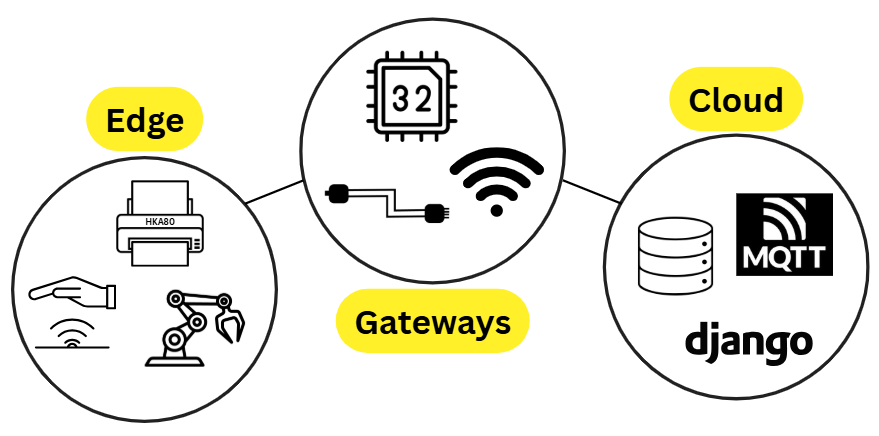
\includegraphics[width=0.8\linewidth]{Img/iiot_diagram.png}
    \caption{Diagrama de los tres niveles fundamentales en un sistema IIoT.}
    \label{fig:imagen1}
\end{figure}

\begin{enumerate}
    \item \textbf{Funcionalidad de borde (Edge):} Sensores y actuadores conectados físicamente a equipos y materiales.
    \item \textbf{Pasarelas de datos (Gateways):} Mecanismos encargados de la recepción y transmisión transparente de información entre los dispositivos de borde y los servidores en red.
    \item \textbf{Gestión y análisis de datos:} Sistemas basados habitualmente en la nube para la recopilación, enlace y análisis de la información para la toma de decisiones.
\end{enumerate}

\par Un pilar en esta arquitectura es la transformación de equipos convencionles en \textbf{productos inteligentes}. Según la Universidad de Cambridge, un activo físico integrado en IIoT posee identidad única \cite{Connected_Everything_2016}, capacidad de comunicación efectiva con su entorno, almacenamiento de datos propio y autonomía para participar en decisiones relevantes para su funcionamiento. Esta metamorfosis de sistemas previamente aislados hacia una red conectada permite recolectar datos \say{no productivos} (como diagnóticos de mantenimiento o estados operativos) que antes eran inaccesibles, optimizando así el ciclo de vida del producto y la eficiencia general del ecosistema industrial.\\

\par Finalmente, la transición de equipos aislados a sistemas hiperconectados introduce una superficie de ataque significativamente mayor, donde la seguridad deja de ser una característica opcional para convertirse en un requisito de diseño mandatorio. El World Economic Forum advierte que el estado de vulnerabilidad en el sector industrial es insostenible sin la adopción de protocolos de seguridad y protección activa \cite{WEF_IIoT_2018}. En el contexto fiscal, donde la integridad de los datos es innegociable, el ecosistema IIoT requiere mecanismos de \say{endurecimiento activo} (active hardening) que garanticen la tríada de la seguridad: confidencialidad, integridad y disponibilidad.\\

\section{Ecosistema de Impresión Fiscal en Venezuela}

\par En el marco legal venezolano, una \textbf{impresora fiscal} no es simplemente un periférico de salida, sino una unidad de control autorizada por el \textbf{SENIAT} para garantizar la integridad de la recaudación tributaria \cite{TheFactoryHKA_Manual_Protocolos}. Bajo normativas como la Providencia 0141, estos equipos son los responsables de emitir documentos con validez legal (facturas, notas de crédito y reportes de cierre diario o \say{Reporte Z}). El corazón de su funcionamiento reside en el \textit{firmware}, un software embebido que regula la interacción entre el hardware de impresión y los módulos de memoria protegida, asegurando que ninguna transacción pueda ser alterada una vez registrada \cite{TheFactoryHKA_Manual_Protocolos, TheFactoryHKA_iSmart_Manual}.

\subsection{Arquitectura modular y Gestión de Memorias}

\par La arquitectura de una impresora fiscal, como la \textbf{HKA80} utilizada en este proyecto, se divide en dos bloques críticos que garantizan la trazabilidad total de las operaciones (vease figura \ref{fig:imagen2}) \cite{TheFactoryHKA_Manual_Protocolos}: 

\begin{figure} [H]
    \centering
    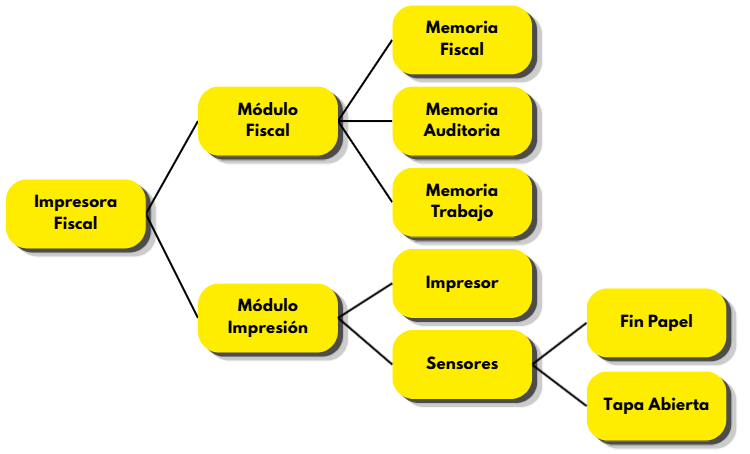
\includegraphics[width=0.9\linewidth]{Img/printer_diagram.png}
    \caption{Estructura de la Impresora Fiscal.}
    \label{fig:imagen2}
\end{figure}

\begin{enumerate}
    \item \textbf{Módulo de Impresión:} Compuesto por el cabezal térmico y sensores de estado (fin de papel, tapa abierta).
    \item \textbf{Módulo fiscal:} El componente más sensible del equipo, encargado de la gestión de tres tipos de memorias independientes:
    \begin{itemize}
        \item \textbf{Memoria Fiscal (MF):} Dispositivo inalterable adherido al chasis que almacena los resúmenes de los Reportes Z, con una cantidad típica de 2000 cierres diarios.
        \item \textbf{Memoria de Auditoría (MA):} Unidad de almacenamiento masivo (generalmente de 2 GB) que guarda copia electrónica fidedigna de cada documento impreso \cite{TheFactoryHKA_Manual_Protocolos}. 
        \item \textbf{Memoria de Trabajo:} Memoria volátil que mantiene los acumuladores de ventas y contadores de la jornada actual, los cuales se transfieren a la MF al ejecutar el cierre diario \cite{TheFactoryHKA_Manual_Protocolos}.
    \end{itemize}
\end{enumerate}

\subsection{Interconexión de Datos: El Rol del Status S1 y SV2}

\par El monitoreo remoto planteado en este trabajo requiere una interconexión física de alto rendimiento para captura de datos en tiempo real. Si bien los sistemas administrativos tradicionales utilizan el estándar serial RS232 para la gestión local \cite{TheFactoryHKA_Manual_Protocolos}, para la integración directa entre el microcontrolador ESP32 y el hardware de la impresora se implementó una \textbf{interfaz de comunicación síncrona}.\\

\par Esta arquitectura de comunicación permite al ESP32 actuar como el controlador principal de la línea, gestionando el flujo de datos mediante señales de sincronismo y control dedicadas. A través de este bus, el firmware realiza el \textit{polling} de información fiscal solicitando tramas específicas como el \textbf{Status S1} (Serial del equipo, RIF y contadores) y \textbf{SV2} (versión de firmware de la impresora) \cite{TheFactoryHKA_Manual_Protocolos, TheFactoryHKA_iSmart_Manual}. La migración no solo garantiza una comunicación de baja latencia y alta confiabilidad, sino que asegura la escalabilidad del sistema ante futuras actualizaciones de hardware, manteniendo la compatibilidad con el dispositivo de transmisión actual de la empresa.

\section{Modelos de Comunicación y Mensajería}

\par En el desarrollo de ecosistemas IIoT, la eficiencia del intercambio de datos depende de la selección de modelos que optimicen el uso del ancho de banda y garantice la integridad de la información. El sistema de transmisión integra tres arquitecturas fundamentales que operan en diferentes niveles de la pila de comunicación, desde la interacción física con el hardware fiscal hasta la visualización en tiempo real en la nube \cite{OASIS_MQTT_v5}.

\subsection{Arquitectura Publicación-Suscripción (Pub/Sub)}

\par A diferencia del modelo tradicional de consulta (request-response), el patrón \textbf{Publicación-Suscripción} desacopla a los productores de datos de los consumidores mediante un intermediario denominado \textit{Broker}, como se muestra en la figura \ref{fig:imagen3} \cite{OASIS_MQTT_v5}. En este proyecto, el microcontrolador ESP32 actúa como publicador de telemetría fiscal, mientras que el Dashboard web se suscribe a tópicos específicos (ej. \texttt{v1/fiscal/serial/json}) para recibir información.\\

\begin{figure} [H]
    \centering
    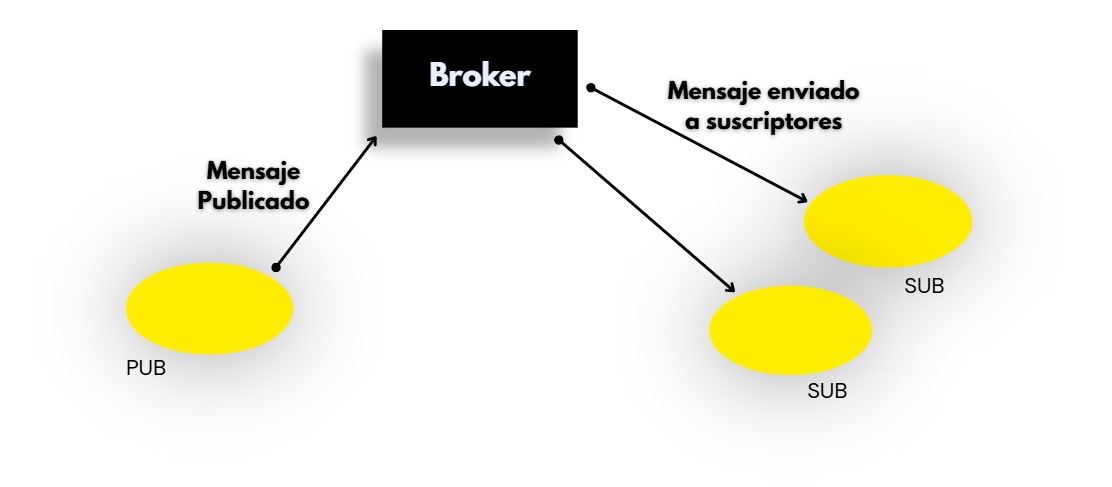
\includegraphics[width=0.95\linewidth]{Img/pubsub_diagram.png}
    \caption{Modelo MQTT de publicación y suscripción.}
    \label{fig:imagen3}
\end{figure}

\par Este modelo ofrece tres dimensiones de desacoplamiento críticas para la robustez industrial \cite{OASIS_MQTT_v5}:

\begin{itemize} 
    \item \textbf{Espacial:} Los dispositivos no necesitan conocer la dirección IP de los demás para comunicarse. 
    \item \textbf{Temporal:} No es necesario que el suscriptor esté en línea al momento de la publicación si se utilizan sesiones persistentes. 
    \item \textbf{Sincronización:} Las operaciones en el ESP32 no se bloquean mientras se envían los datos, permitiendo que la tarea de la impresora continúe su ejecución. 
\end{itemize}

\subsection{Comunicación Bidireccional Full-Duplex (WebSockets)}

\par Para el monitoreo en tiempo real, se implementó el protocolo \textbf{WebSockets}, el cual establece un canal de comunicación persistente y bidireccional sobre una única conexión TCP \cite{RFC6455_WebSockets, Fierro_WebSockets_2017}. A diferencia de HTTP, que requiere una nueva cabecera por cada solicitud, WebSockets reduce drásticamente la latencia mediante un proceso de \textit{handshake} que eleva la conexión de HTTP a un flujo de datos binarios continuo.\\

\par En la arquitectura final de este proyecto, se utiliza \textbf{MQTT sobre WebSockets} \cite{OASIS_MQTT_v5, Fierro_WebSockets_2017}. Esta técnica permite que el Dashboard web encapsule paquetes MQTT dentro de tramas de WebSocket, permitiendo que el navegador \say{hable} directamente con el broker. Esto elimina la necesidad de intermediarios pesados (como Django Channels), simplificando la infraestructura y garantizando que los estados de la impresora se reflejen en pantalla de forma instantanea.

\subsection{Modelo Maestro-Esclavo en Buses Seriales}

\par En el nivel del borde (\textit{Edge}), la interacción entre el microcontrolador y la impresora fiscal se rige por el modelo \textbf{Maestro-Esclavo} \cite{TheFactoryHKA_Manual_Protocolos}. En esta jerarquía, el ESP32 asume el rol de maestro, teniendo el control total sobre el bus de comunicación y decidiendo cuando iniciar la transferencia de datos.\\

\par Para la integración con la impresora HKA80, este modelo se manifiesta a través de un \textbf{bus de comunicación serie síncrono}. El controlador principal genera la \textbf{señal de temporización} y gestiona la \textbf{habilitación del dispositivo periférico} para realizar un  un sondeo \textit{polling} constante de los registros fiscales. Si bien este modelo presenta una alta dependencia del maestro, garantiza un determinismo absoluto en la captura de datos críticos, evitando colisiones en el bus y asegurando que cada trama de \textbf{Status S1} sea recibida y validada antes de proceder con la lógica de red.

\section{Hardware de Alto Rendimiento: ESP32}

\par El núcleo del sistema de transmisión se fundamenta en el ESP32, un sistema en chip (SoC) de bajo consumo diseñado por Espressif Systems que integra conectividad Wi-Fi y Bluetooth de modo dual \cite{Espressif_ESP32_Datasheet}. A diferencia de los microcontroladores convencionales, este dispositivo está diseñado para aplicaciones industriales de IoT, ofreciendo una robustez y versatilidad que permiten manejar simultáneamente tareas de comunicación segura y control de periféricos de alta velocidad (véase la Figura \ref{fig:esp32_physic}).

\begin{figure} [H]
    \centering
    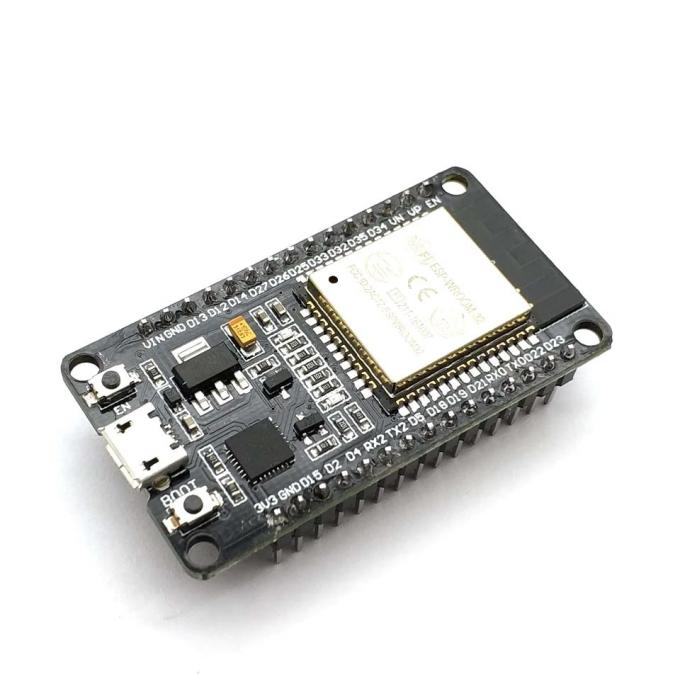
\includegraphics[width=0.5\linewidth]{Img/esp32_physic.png}
    \caption{Vista realista del microcontrolador ESP32.}
    \label{fig:esp32_physic}
\end{figure}

\subsection{Arquitectura de Procesamiento y Multitarea (FreeRTOS)} 

\par El dispositivo integra un microprocesador Xtensa Dual-Core LX6 de 32 bits, capaz de alcanzar un rendimiento de hasta 600 MIPS \cite{Espressif_ESP32_Datasheet}. Esta arquitectura de doble núcleo es un pilar en el proyecto, ya que permite la implementación de un sistema operativo de tiempo real (FreeRTOS) \cite{FreeRTOS_Kernel_Ref}. Mediante la gestión de tareas independientes, el firmware separa la lógica de captura de datos fiscales (tarea de prioridad 5) del stack de comunicación de red, garantizando que el polling de la impresora no se vea interrumpido por las latencias inherentes a la comunicación en la nube.

\subsection{Jerarquía de Memoria y Optimización Crítica} 

\par La gestión de la memoria es el factor determinante para la estabilidad de sistemas que emplean MQTT v5.0 y cifrado TLS/SSL. El ESP32 cuenta físicamente con 520 KB de SRAM interna, la cual se distribuye de forma lógica para optimizar el rendimiento del sistema \cite{Espressif_ESP32_Datasheet}:

\begin{itemize} 
    \item \textbf{IRAM (Instruction RAM):} Espacio de 128 KB reservado para instrucciones críticas y manejadores de interrupciones. El uso eficiente de la IRAM es determinante en sistemas embebidos industriales para alojar stacks de seguridad como Mbed TLS sin comprometer la estabilidad del sistema \cite{Espressif_ESP32_Datasheet}.
    \item \textbf{DRAM (Data RAM):} Utilizada para buffers de datos y el \textit{heap} de la aplicación. Para garantizar la robustez ante fallos de energía, el sistema emplea la \textbf{NVS Flash} (memoria no volátil) para almacenar configuraciones críticas que deben persistir tras un reinicio \cite{Espressif_ESP_IDF_v552}. 
\end{itemize}

\subsection{Seguridad por Hardware y Aceleración Criptográfica}

\par El despliegue de dispositivos IoT en infrestructuras fiscales introduce vulnerabilidades críticas que deben ser mitigadas mediante estándares de crifrado robustos. Sin embargo, la ejecución de algoritmos como AES (Advanced Encryption Standard) o SHA-2 (Secure Hash Algorithm) mediante software consume ciclos de reloj significativos, lo que puede elevar el consumo energético y generar latencia \cite{Espressif_ESP32_Datasheet}.\\

\par El uso de \textbf{Aceleradores Criptográficos por Hardware} en microcontroladores modernos permite delegar estas operaciones matemáticas complejas a módulos de silicio dedicados \cite{Espressif_ESP32_Datasheet, NIST_SP800_52}. Esto garantiza:

\begin{itemize}
    \item \textbf{Integridad de Datos:} Asegura que los registros fiscales no sean alterados durante el tránsito hacia la nube.
    \item \textbf{Autenticación Mutua:} Facilita el intercambio de certificados digitales en el protocolo TLS/SSL de forma eficiente, permitiendo que solo dispositivos autorizados se comuniquen con el servidor central \cite{RFC5246_TLS12}. 
\end{itemize}

\subsection{Interfaces de Comunicación y Capacidad Sensorial} 

\par El sistema de transmisión aprovecha la matriz de periféricos avanzados del chip para la integración con el ecosistema fiscal \cite{Espressif_ESP32_Datasheet}. Se utiliza una interfaz de comunicación física operando a una frecuencia optimizada, lo que asegura un intercanbio de datos constante y de baja latencia con hardware de impresión. Esta interfaz permite al ESP32 actuar como el maestro de la comunicación, gestionando líneas dedicadas para la captura inmediata de registros de estado.\\

\par Asimismo, la radio integrada de 2.4 GHz permite la interconexión bajo los estándares 802.11 b/g/n, posicionando al dispositivo como un Gateway industrial que cumple con las capas de detección e intercambio de datos descritas en la arquitectura IoT industrial \cite{Espressif_ESP32_Datasheet}.

\section{Desarrollo Profesional con ESP-IDF y FreeRTOS}

\par A diferencia de los entornos de prototipado rápido, la implementación de un sistema de monitoreo fiscal industrial exige un control granular sobre los recursos del hardware y una ejecución determinista de las tareas. Por ello, este proyecto se fundamenta en el \textbf{Espressif IoT Development Framework (ESP-IDF)}, el entorno de desarrollo nativo que permite explotar la arquitectura de doble núcleo del ESP32 mediante el uso de un \textbf{Sistema Operativo de Tiempo Real (FreeRTOS)} \cite{Espressif_ESP_IDF_v552, FreeRTOS_Kernel_Ref}.

\subsection{Gestión de Tareas y Sincronización (Mutexes y Colas)}

\par En entornos industriales, el monitoreo de equipos fiscales exige una ejecución determinística. El uso de un RTOS (Real-Time Operating System) como FreeRTOS permite la abstracción del hardware mediante la implementación de un planificador de tareas (\textit{Scheduler}) basado en prioridades \cite{FreeRTOS_Kernel_Ref}. Esta arquitectura es fundamental para garantizar que los procesos de comunicación no bloqueen la lectura crítica de datos fiscales.\\

\par La robustez del firmware se fundamenta en tres pilares conceptuales de la computación concurrente haciendo que las tareas se fragmenten tal como muestra la figura \ref{fig:imagen4}:

\begin{figure} [H]
    \centering
    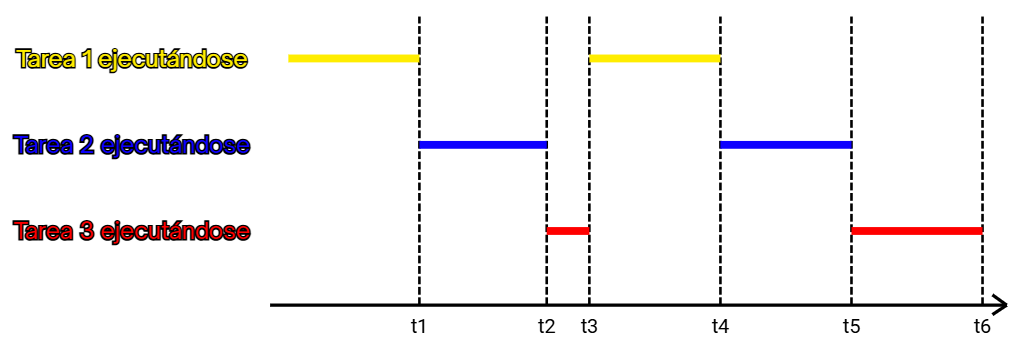
\includegraphics[width=0.9\linewidth]{Img/scheuler_diagram.png}
    \caption{Diagrama de ejecución de tres tareas en distintos instantes de tiempo.}
    \label{fig:imagen4}
\end{figure}

\begin{itemize}
    \item \textbf{Planificación por Prioridades (Preemptive Scheduling):} Permite que el procesador alterne entre múltiples hilos de ejecución. En sistema IoT, esto asegura que las tareas de alta prioridad, como el procesamiento de tramas de comunicación como la impresora, se ejecuten imediantamente, mientras que las tareas de menor prioridad, como el envío de telemetría, se procesen en los tiempos de espera del CPU \cite{FreeRTOS_Kernel_Ref}.
    \item \textbf{Mecanismos de Exclusión Mutua (Mutex):} El acceso concurrente a recursos compartidos, como los buses de comunicación, representa un riesgo de corrupción de datos. El uso de \textit{Mutexes} garantiza que solo una tarea posea el control del recurso en un momento dado, evitando condiciones de carrera (\textit{race conditions}) que podrían comprometer la integridad de la información tributaria \cite{FreeRTOS_Kernel_Ref}.
    \item \textbf{Sincronización mediante Semáforos y Colas (Queues):} Estos mecanismos permiten la comunicación inter-tareas. Las colas de mensajes facilitan el paso de datos entre el núcleo que gestiona la lógica de la impresora y el núcleo encargado de la pila de red, permitiendo una arquitectura desacoplada y escalable \cite{FreeRTOS_Kernel_Ref}.
\end{itemize}

\section{Protocolos de Red y Transporte}

\par La arquitectura de comunicaciones del sistema de transmisión se fundamenta en una pila de protocolos diseñados para entornos de alta confiabilidad y recursos restringidos. La integración del estándar \textbf{MQTT v5.0} sobre capas de seguridad \textbf{TLS/SSL}, sumada a la eficiencia del bus para la comunicación local, constituye una infraestructura robusta que garantiza la integridad de la información fiscal desde el borde hasta la nube \cite{OASIS_MQTT_v5, RFC5246_TLS12}.

\subsection{MQTT v5.0: Características Avanzadas y Trazabilidad}

\par El protocolo \textbf{MQTT (Message Queuning Telemetry Transport)} es un estándar de mensajería basado en el modelo publicación-suscripción, optimizado para redes de baja tasa de bits y alta latencia \cite{OASIS_MQTT_v5}. Para este proyecto, se implementó la versión \textbf{5.0}, la cual representa una evolución crítica respecto a su predecesor (v3.1.1), introduciendo características de escalabilidad y reporte de errores superiores.\\

\par Una de las herramientas integradas en el firmware es el uso de las \textbf{User Properties}. Estas permiten adjuntar metadatos personalizados en formato clave-valor a las tramas de publicación (PUBLISH), facilitando una \textbf{trazabilidad transparente} en sistemas complejos. En el sistema de transmisi\'on, estas propiedades se utilizan para enviar información de autodiagnóstico y modelo de hardware sin sobrecargar el \textit{payload} JSON del mensaje. Además, el uso de \textbf{Reason Codes} en todos los paquetes de reconocimiento (ACKs) permite que el ESP32 reciba una retoralimentación detallada del broker ante cualquier fallo de comunicación, mejorando la resilencia operativa del nodo sensor \cite{OASIS_MQTT_v5}.

\subsection{Seguridad en la Capa de Transporte (TLS/SSL)}

\par Dado que el sistema maneja información tributaria sensible, la seguridad es un requisito de diseño mandatorio. El sistema utiliza el protocolo \textbf{Transport Layer Security (TLS)}, su sucesor del Secure Socket Layer (SSL), para proporcionar un canal cifrado sobre TCP que garantiza la \textbf{confidencialidad, integridad, y autenticidad} de los datos \cite{RFC5246_TLS12, NIST_SP800_52}.\\

\par La implementación se basa en un proceso de \textbf{Handshake} mediante el cual el ESP32 y el broker negocian parámetros criptográficos y validan identidades a través de certificados digitales. Siguiendo las recomendaciones internacionales, el sistema opera sobre el \textbf{puerto seguro 8883} (IANA: \textit{secure-mqtt}), lo que mitiga riesgos criticos como el espionaje pasivo (\textit{eavesdropping}) y la inyección de contenido malicioso \cite{NIST_SP800_52}. Esta capa de seguridad asegura que, incluso si las tramas son interceptadas en la red pública, la información permanezca ininteligible para atacantes externos.

\subsection{Comunicación Serial e Interfaz de Datos Local}

\par En el nivel de borde, la captura de datos fiscales se realiza a través una \textbf{interfaz de comunicación síncrona de alto rendimiento} \cite{TheFactoryHKA_Manual_Protocolos}. A diferencia de las interfaces seriales asíncronas tradicionales (UART), este método permite el intercambio de información en modo \textit{full-duplex} con un determinismo superior.\\

\par El sistema de transmisi\'on opera bajo una jerarquía de \textbf{Maestro-Esclavo}, donde el microcontrolador ESP32 actúa como el nodo maestro que genera la señal de \textbf{sincronización (o temporización)} y gestiona la línea de \textbf{habilitación del periférico} para orquestar la comunicación con la impresora fiscal. Esta arquitectura garantiza un determinismo absoluto en la captura de registros críticos (Status S1/SV2), ya que el uso de \textbf{vías de transmisión y recepción independientes} evita colisiones de datos y permiten velocidades de transferencia significativamente superiores a las de una conexión RS232 convenicional \cite{TheFactoryHKA_Manual_Protocolos}. El uso de este bus síncrono es lo que permite que el sistema mantenga una frecuencia de muestreo constante de 5 segundos sin interferir con las operaciones internas del firmware de la impresora.

\section{Estructuraci\'on de Datos con JSON}

\par En la arquitectura de comunicaciones de este proyecto, la representac\'on y el empaquetado de la informaci\'on fiscal se fundamentan en el formato \textbf{JSON (JavaScript Object Notation)}. Este es un est\'andar de intercambio de datos ligero, basado en una estructura de pares clave-valor, que permite una legibilidad superior tanto para humanos como para m\'aquinas \cite{Salazar_IoT_2014}. Su adopción en sistemas IIoT es cr\'itica debido a su independencia de lenguaje, lo que facilita la interoperabilidad entre el firmware desarrollado en \textbf{C (ESP-IDF)}, el broker MQTT y el backend en \textbf{Python (Django)}.\\

\par A diferencia de otros lenguajes del mercado como XML, JSON ofrece una sobrecarga (\textit{overhead}) significativamente menor, lo que se traduce en paquetes m\'as pequeños y un menor consumo de energ\'ia y memoria en el microcontrolador \cite{Salazar_IoT_2014}. En el sistema de transmisi\'on, los paquetes JSON se encapsulan tanto en tramas MQTT como en sobres de WebSockets para su transporte hacia la nube.

\section{Integración Web y Monitoreo en Tiempo Real}

\par La capa de visualizaci\'on del sistema de transmisi\'on trasciende los portales web est\'aticos mediante la implementaci\'on de tecnolog\'ias de flujo de datos continuo. El uso de protocolos de baja latencia garantiza que los estados de la impresora fiscal se reflejen en el Dashboard con un retraso imperceptible, cumpliendo con los est\'andares de monitoreo industrial en tiempo real \cite{RFC6455_WebSockets}.

\subsection{Protocolo WebSockets}

\par El protocolo \textbf{WebSocket}, definido en el RFC 6455, proporciona canales de comunicaci\'on \textbf{full-duplex} sobre una \'unica conexi\'on TCP \cite{RFC6455_WebSockets}. A diferencia del protocolo HTTP, que es de naturaleza \textit{half-duplex} y carece de estado, WebSocket permite que el servidor env\'ie informaci\'on al cliente de forma proactiva sin esperar una solicitud previa.\\

\par El establecimiento de la comunicaci\'on se rige por el proceso \textbf{Handshake}, el cual inicia como una solicitud HTTP convencional. Durante este intercambio, el cliente y el servidor acuerdan una \say{actualizaci\'on de protocolo} (\textit{Protocol Upgrade}), transformando la conexi\'on HTTP en un flujo de datos binarios bidireccional y persistente. Una vez establecida, se eliminan la cabeceras (\textit{headers}) repetitivas de HTTP, lo que reduce dr\'asticamente el payload de la conexi\'on y permite una transferencia de datos m\'as eficiente y con menor latencia en comparaci\'on con t\'ecnicas como el \textit{long polling} \cite{Fierro_WebSockets_2017}.

\subsection{MQTT sobre WebSockets}

\par En la arquitectura final de este proyecto, se implement\'o la t\'ecnica de \textbf{t\'unel o encapsulamiento de MQTT sobre WebSockets}. Esta integraci\'on es fundamental debido a que los navegadores web actuales no permiten la apertura de conexione TCP crudas (\textit{raw sockets}) necesarias para el protocolo MQTT nativo \cite{OASIS_MQTT_v5, Fierro_WebSockets_2017}.\\

\par Bajo este esquema, la conexi\'on WebSocket act\'ua como una tuber\'ia externa o \say{sobre} para los paquetes MQTT. El broker HiveMQ coloca cada paquete MQTT (como CONNECT o PUBLISH) dentro de una trama binaria de WebSocket para enviarla al Dashboard, donde la librer\'ia de cliente JavaScript (Paho) desaempaqueta la informaci\'on y la procesa como una trama de red est\'andar \cite{OASIS_MQTT_v5}. En el sistema de transmisi\'on, esta comunicaci\'on segura se orquesta a trav\'es del \textbf{puerto 8000}, lo que permite atravesar firewalls corporativos que habitualmente bloquean los puertos est\'andar de MQTT (1883/8883) pero permiten el tr\'afico web convencional. Esta arquitectura desacoplada garantiza la \textbf{resilencia cibern\'etica} del sistema, permitiendo un monitoreo directo entre el navegador y el broker sin intermediarios adicionales.

\section{Arquitectura de Gesti\'on y Orquestaci\'on: Framework Django}

\par La capa superior del ecosistema de transmici\'on requiere de un motor robusto capaz de centralizar la informaci\'on, gestionar la seguridad de acceso y servir de puente entre el almacenamiento de datos y la interfaz de usuario. Para este prop\'osito, se seleccion\'o \textbf{Django}, un framework web de alto nivel basado en el lenguaje de programaci\'on \textbf{Python} \cite{Django_v5_Doc}. Python se caracteriza por ser un lenguaje interpretado de prop\'osito general, cuya filosof\'ia hace hincap\'ie en la legibilidad del c\'odigo y la eficiencia t\'ecnica, caracter\'isticas esenciales para el mantenimiento de sistemas industriales a largo plazo.

\subsection{Patr\'on de Diseño MVT (Model-View-Template)}

\par Django fundamenta su operaci\'on en una arquitectura denominada \textbf{Model-View-Template}, la cual permite una separaci\'on clara de responsabilidades en el servidor de aplicaciones \cite{Django_v5_Doc}:

\begin{itemize}
    \item \textbf{Modelo (Model):} Representa la fuente de informaci\'on definitiva de los datos. En este proyecto, el modelo define la estructura de las tablas donde se gestionan los equipos fiscales y los registros de auditor\'ia.
    \item \textbf{Vista (View):} Act\'ua como el mediador l\'ogico que procesa las solicitudes de los usuarios y retorna las respuestas adecuadas. Es el componente encargado de la orquestaci\'on del sistema.
    \item \textbf{Plantilla (Template):} Es la capa de presentaci\'on que define c\'omo se muestran los datos al usuario final, integrando el contenido generado por el servidor con el Dashboard web.
\end{itemize}

\subsection{Arquitectura Web Eficiente: HTMX y la comunicación Asíncrona}

\par En la evolución del desarrollo web para sistemas embebidos, ha surgido una dicotomía entre las aplicaciones tradicionales multipágina (MPA) y las aplicaciones de una sola página (SPA) basadas en pesados \textit{frameworks} de JavaScript. HTMX se presenta como una alternativa que permite extender las capacidades del HTML para realizar peticiones AJAX, WebSockets y Server-Sent Events directamente desde los atributos del mercado \cite{HTMX_Doc}.\\

\par La relevancia de HTMX en este proyecto radica en:

\begin{itemize}
    \item \textbf{Reducción de la Carga en el Cliente:} Al procesar la lógica de presentación en el servidor (Django) y enviar solo fragmentos de HTML al navegador, se minimiza la necesidad de procesar grandes archivos de \textit{scripts} en el dispositivo del usuario final.
    \item \textbf{Reactividad sin Complejidad:} Permite actualizaciones parciales del Dashboard web (como el estado de conexión de la impresora) en tiempo real, manteniendo la simplicidad del protocolo HTTP sin la sobrecarga de un motor de renderizado del lado del cliente.
\end{itemize}

\subsection{Gesti\'on Administrativa y Persistencia}

\par Una de las caracter\'isticas de este framework es su capacidad de generar din\'amicamente una \textbf{interfaz administrativa} (Admin Panel). Esta herramienta permite que los administradores del sistema en \textbf{The Factory HKA} realicen operaciones \textbf{CRUD} (Crear, Leer, Actualizar y Borrar) sobre la base de datos de los equipos de forma segura, sin necesidad de interactuar directamente con el motor de base de datos SQL \cite{Django_v5_Doc}.\\

\par En la arquitectura del dispositivo de transmisión, Django cumple el rol de Servidor de Aplicaciones, diferenci\'andose de un servidor web est\'atico al procesar l\'ogica compleja y garantizar que solo usuarios autenticados puedan acceder al monitoreo en tiempo real de los registros fiscales. Esta robustez, sumada a su enfoque en la reutilizaci\'on de componentes y el principio \textit{don't repeat yourself} (DRY), asegura que el sistema sea escalable ante el crecimiento del parque de impresoras instaladas \cite{Django_v5_Doc}.
    \chapter{DESARROLLO}

\section{Diseño Conceptual de la Arquitectura IIoT}
\label{sec:diseno_conceptual}

    \par El diseño conceptual del Módulo de Transmisión IoT (MT-IoT) se fundamenta en la necesidad de transformar equipos de control fiscal, tradicionalmente aislados, en nodos inteligentes capaces de integrarse a una red de monitoreo centralizada. Tal como se estableció en el plan de trabajo durante las semanas 3 y 4, el objetivo fue definir los planos técnicos y lógicos para posicionar al microcontrolador ESP32 como un puente (\textit{Gateway}) entre el hardware fiscal y la nube \cite{WEF_IIoT_2018, Connected_Everything_2016}.\\

    \par El desarrollo del proyecto se organizó en cuatro fases metodológicas sucesivas, cuyo flujo general se resume en la Figura \ref{fig:flujo_metodologico}:

    \begin{figure}[htbp]
    \centering
    \begin{tikzpicture}[node distance=0.6cm, auto, >=latex',
        phase/.style={rectangle, draw, rounded corners, fill=blue!10, text width=9.5cm, align=center, minimum height=1.0cm, font=\small},
        ar/.style={thick,->,>=stealth}]
        \node [phase] (f1) {\textbf{Fase 1.} Levantamiento de Requerimientos y Simulación HIL};
        \node [phase, below=of f1] (f2) {\textbf{Fase 2.} Detección de Inestabilidades y Cuellos de Botella (IRAM / EMI)};
        \node [phase, below=of f2] (f3) {\textbf{Fase 3.} Re-ingeniería del Kernel Concurrente (FreeRTOS / Mutex)};
        \node [phase, below=of f3] (f4) {\textbf{Fase 4.} Despliegue del Ecosistema Cloud (Django / HTMX / MQTT v5.0)};
        \draw [ar] (f1) -- (f2);
        \draw [ar] (f2) -- (f3);
        \draw [ar] (f3) -- (f4);
    \end{tikzpicture}
    \caption{Flujo metodológico general del trabajo de pasantía organizado en cuatro fases sucesivas.}
    \label{fig:flujo_metodologico}
    \end{figure}

    Para garantizar la escalabilidad y robustez del sistema (véase la Figura \ref{fig:arquitectura_iiot}), se optó por una arquitectura distribuida de tres niveles, alineada con los estándares industriales del Internet de las Cosas (IIoT) \cite{WEF_IIoT_2018, Connected_Everything_2016}:
    
    \begin{itemize}
        \item \textbf{Nivel de Borde (Edge):} Representado por la impresora fiscal HKA80. En esta capa se origina la información crítica mediante registros de estado (\texttt{Status S1}) y diagnóstico (\texttt{SV2}) \cite{TheFactoryHKA_Manual_Protocolos}. La captura de estos datos se realiza a través de una interfaz de comunicación síncrona de alto rendimiento, diseñada para operar de forma transparente. Esta transparencia se logra manteniendo un intervalo de sondeo (\textit{polling}) estrictamente acotado, asegurando que los tiempos de respuesta de la transacción no excedan los umbrales de latencia tolerados por el \textit{firmware} legal del equipo; premisa que será demostrada posteriormente mediante un perfilado de tiempos en el bus de datos.

        \item \textbf{Nivel de Pasarela (Gateway):} Ejecutado por el Módulo de Transmisión IoT (basado en el SoC ESP32). Su función es doble: actúa como maestro en la interfaz local con el periférico y como cliente seguro (\textit{Publisher}) hacia la red Wi-Fi \cite{Espressif_ESP32_Datasheet}. En este nivel se implementa la lógica de empaquetado de datos en formato JSON y la gestión de seguridad mediante TLS/SSL, permitiendo el acceso a registros críticos almacenados en la Memoria de Trabajo y Memoria de Auditoría sin interferir con el cabezal de impresión.

        \item \textbf{Nivel de Gestión y Visualización (Cloud):} Compuesto por el \textit{Broker} HiveMQ y el servidor de aplicaciones desarrollado en Django \cite{Django_v5_Doc}. Este nivel orquesta la recepción asíncrona de telemetría y su visualización en tiempo real en el Dashboard mediante un túnel de \textit{MQTT sobre WebSockets} \cite{OASIS_MQTT_v5, RFC6455_WebSockets}.
    \end{itemize}

    \begin{figure}[htbp]
        \centering
        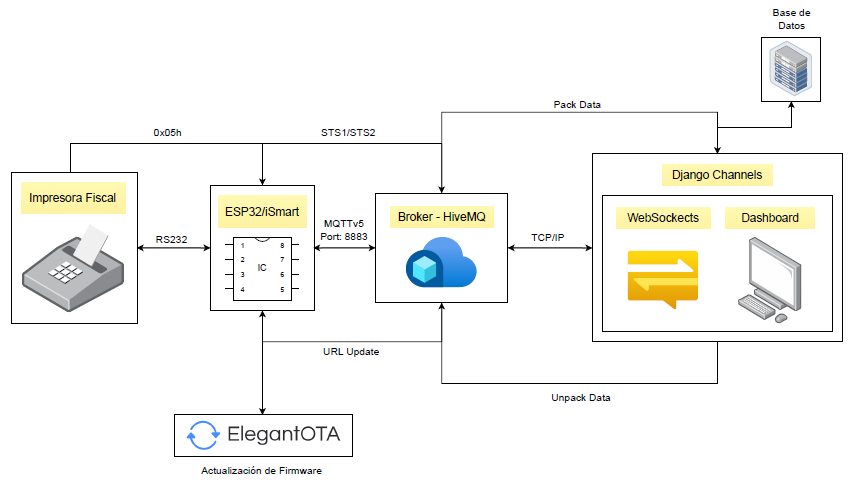
\includegraphics[width=0.95\textwidth]{Img/arquitectura_iiot.png} 
        \caption{Diagrama de la Arquitectura IIoT distribuida en tres niveles (Edge, Gateway y Cloud).}
        \label{fig:arquitectura_iiot}
    \end{figure}

    \par La elaboración de los diagramas técnicos (Figura \ref{fig:arquitectura_iiot} y Figura \ref{fig:arquitectura_mqtt}) respondió a la necesidad de visualizar el flujo de datos desde el comando inicial \texttt{0x05h} (ENQ) enviado por el MT-IoT hasta el desempaquetado (\textit{Unpack Data}) en la plataforma web \cite{Connected_Everything_2016}. El diseño de la arquitectura de comunicaciones fue especialmente crítico para definir el \textit{Topic Tree} (jerarquía de tópicos) y el uso de \textit{User Properties} de MQTT v5.0 \cite{OASIS_MQTT_v5}. La inyección de metadatos (como la versión del firmware y la intensidad de señal Wi-Fi) directamente en las \textit{User Properties} de la cabecera del protocolo evita sobrecargar el cuerpo del mensaje JSON, lo cual reduce significativamente el consumo de ancho de banda y elimina la necesidad de \textit{parsing} adicional en el servidor \cite{OASIS_MQTT_v5}.

    \begin{figure}[H]
        \centering
        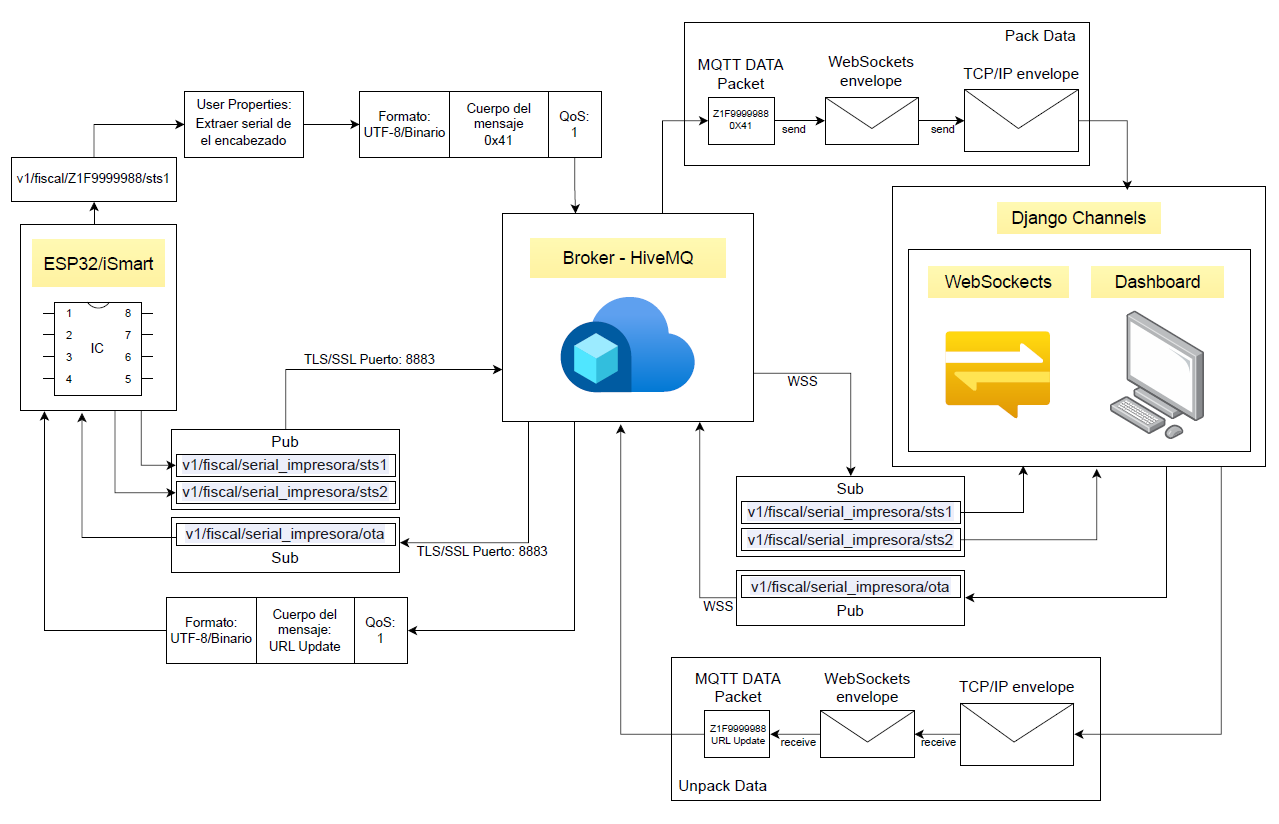
\includegraphics[width=0.95\textwidth]{Img/arquitectura_mqtt.png}
        \caption{Diagrama propuesto para la arquitectura de comunicaciones MQTT.}
        \label{fig:arquitectura_mqtt}
    \end{figure}

\section{Análisis de Decisiones de Arquitectura y Compromisos de Ingeniería}

\subsection{Microcontrolador de Doble Núcleo: ESP32}

\par Para la implementación del nodo de transmisión, se seleccionó la tarjeta de desarrollo ESP32 DevKitC V4. Esta elección se fundamentó en la necesidad de gestionar procesos concurrentes industriales \cite{Espressif_ESP32_Datasheet, FreeRTOS_Kernel_Ref}. En la arquitectura final, se asignaron tareas específicas a cada núcleo para garantizar el determinismo: mientras un núcleo gestiona el sondeo (\textit{polling}) de la impresora fiscal cada 5 segundos, el segundo núcleo administra la pila de red y la mensajería MQTT v5.0, evitando que las latencias de internet bloqueen la captura de datos locales.\\

\par Durante el prototipado, se identificó una limitación crítica en el hardware relacionada con la asignación de periféricos. Al intentar utilizar el UART1 en sus pines por defecto (GPIO 9 y 10), el sistema experimentaba reinicios constantes (bootloops) debido a que estos pines están anclados al bus SPI de la memoria Flash interna del SoC \cite{Espressif_ESP32_Datasheet}. Para solventar esta colisión eléctrica, se reconfiguró la matriz de señales, moviendo la interfaz de comunicación fiscal hacia los pines libres GPIO 18 (TX) y GPIO 19 (RX), logrando una transmisión estable (véase la Figura \ref{fig:pinlayout}).\\

\begin{figure}[htbp]
    \centering
    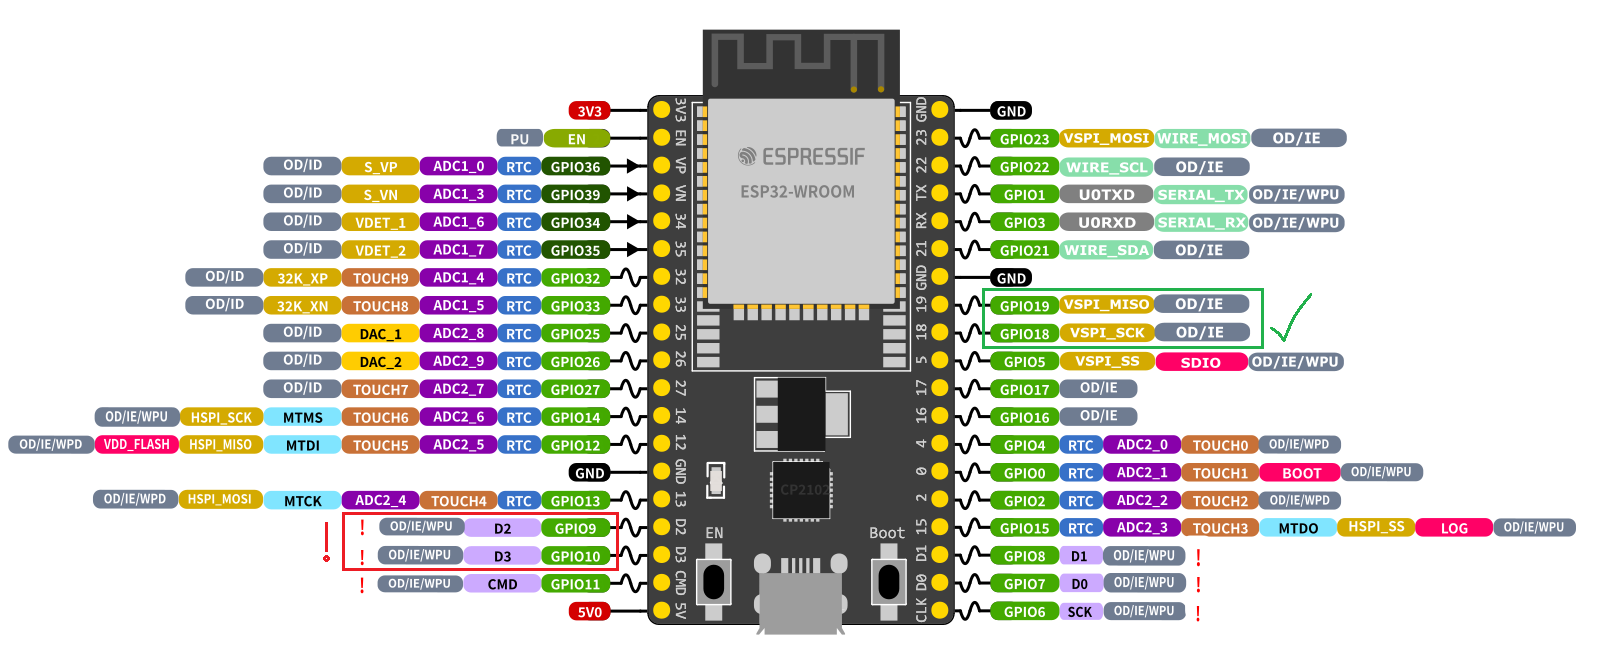
\includegraphics[width=0.8\linewidth]{Img/esp32_pinlayout.png}
    \caption{Pinlayout de la tarjeta ESP32 DevKitC V4 y reasignación de pines seriales.}
    \label{fig:pinlayout}
\end{figure}

\par La gestión de la memoria interna representó el mayor desafío técnico. Con la implementación completa de la pila TLS/SSL y el empaquetado dinámico de mensajes JSON, el uso de la memoria IRAM alcanzó un nivel crítico del 78.39\% en la semana 6. Tras un análisis de perfilado del \textit{firmware}, se aplicó una reingeniería de recursos mediante la herramienta \texttt{menuconfig} desactivando la aceleración IRAM para el \textit{stack} Wi-Fi (véase la Figura \ref{fig:menuconfig_wifi}). Esta decisión redujo el consumo de memoria a un 52.26\% (un ahorro directo del 26.13\%), liberando el \textit{heap} necesario para alojar el búfer de actualización remota (OTA).

\begin{figure}[htbp]
    \centering
    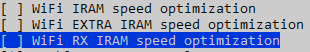
\includegraphics[width=0.5\linewidth]{Img/menuconfig_optimizacion_wifi.png}
    \caption{Configuración aplicada en menuconfig para optimización de IRAM.}
    \label{fig:menuconfig_wifi}
\end{figure}

\par Finalmente, para optimizar el consumo energético y la disipación térmica en operación continua, se aplicó una técnica de \textit{underclocking}, ajustando la frecuencia del CPU a 80 MHz (vease Figura \ref{fig:menuconfig_under}) \cite{Espressif_Menuconfig}. Esta frecuencia demostró ser estadísticamente suficiente para sostener la aceleración criptográfica de AES por hardware requerida por la conexión segura hacia HiveMQ.

\begin{figure}[htbp]
    \centering
    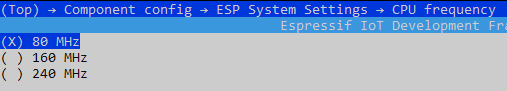
\includegraphics[width=0.7\linewidth]{Img/menuconfig_optimizacion_under.png}
    \caption{Underclocking aplicado en menuconfig para optimización de consumo energético.}
    \label{fig:menuconfig_under}
\end{figure}

\subsection{Unidad de Control Fiscal: Impresora HKA80}

\par La impresora fiscal HKA80 (véase la Figura \ref{fig:hka80}) actúa como el activo de borde (\textit{Edge}) central del sistema. Su selección se fundamentó en su arquitectura modular, la cual permite el acceso a registros críticos almacenados en su Memoria de Trabajo y Memoria de Auditoría sin interrumpir mecánicamente al cabezal de impresión.

\begin{figure}[htbp]
    \centering
    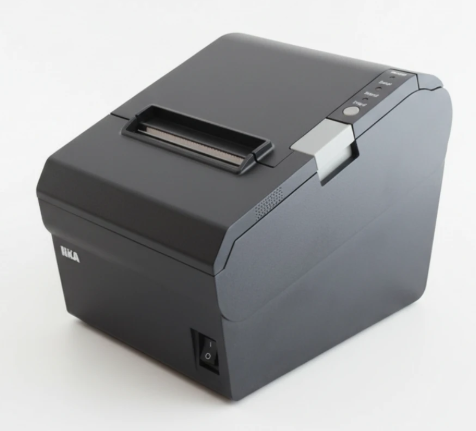
\includegraphics[width=0.6\linewidth]{Img/hka80.png}
    \caption{Impresora fiscal modelo HKA80 autorizada por la normativa vigente.}
    \label{fig:hka80}
\end{figure}

\par Para la integración con el MT-IoT, se definieron los parámetros obligatorios del protocolo: tasa de transferencia de 9600 bps, longitud de 8 bits, paridad par y 1 bit de parada \cite{TheFactoryHKA_Manual_Protocolos}. La fase inicial de la telemetría priorizó el registro \texttt{Status S1} (identidad del equipo y acumuladores) y el comando \texttt{SV2} (versión de \textit{firmware} del periférico).\\

\par Un hallazgo crítico durante el desarrollo del \textit{parser} fue la identificación de un carácter invisible de salto de línea (\texttt{\textbackslash n}) inmediatamente antes del fin de trama (ETX) emitido por la impresora. Este factor desplazaba los punteros de memoria provocando errores de tipo \textit{Off-By-One}, los cuales corrompían el \textit{payload} MQTT. La anomalía fue resuelta introduciendo un ajuste dinámico que inyecta un terminador nulo en la memoria RAM para purgar la trama. La secuencia analítica de esta corrección se describe en el Algoritmo \ref{alg:offbyone}, mientras que su implementación en lenguaje C se conserva en el Apéndice \ref{apx:codigo}.

\begin{algorithm}[htbp]
\caption{Mitigación analítica del error Off-By-One en el parseo de la trama SV2.}
\label{alg:offbyone}
\begin{algorithmic}[1]
\State Recibir el bloque de respuesta y validar su redundancia (LRC).
\State Calcular la posición del terminador: $p_{ETX} \leftarrow n - 2$.
\State Estimar el índice inicial del campo de versión: $i_0 \leftarrow p_{ETX} - L_{fw} - 1$.
\If{$i_0 \geq 1$}
    \State Reservar la sección crítica de memoria.
    \State Copiar $L_{fw}$ caracteres desde $i_0$ hacia el campo de versión.
    \State Inyectar el terminador nulo manual en la posición $L_{fw}$.
    \State Liberar la sección crítica.
    \State \Return verdadero
\EndIf
\State \Return falso
\end{algorithmic}
\end{algorithm}

\par Esta sanitización de datos asegura un determinismo absoluto en la captura de registros cada 5 segundos, permitiendo que el MT-IoT actúe como un \textit{Gateway} transparente que no añade latencia a la red transaccional del contribuyente.

\subsection{Justificación del Framework Nativo: Determinismo vs. Latencia (ESP-IDF)}

\par Durante la semana de definición tecnológica se realizó un análisis comparativo entre el entorno Arduino IDE y el Espressif IoT Development Framework (ESP-IDF) (véase la Tabla \ref{tab:comparativa_frameworks}).\\

\begin{table}[htbp]
    \centering
    \caption{Análisis comparativo de entornos de desarrollo para el nodo Gateway.}
    \label{tab:comparativa_frameworks}
    \begin{tabularx}{\textwidth}{@{}>{\raggedright\arraybackslash}p{3.0cm} >{\raggedright\arraybackslash}X >{\raggedright\arraybackslash}X@{}}
        \toprule
        \textbf{Criterio} & \textbf{Arduino IDE} & \textbf{ESP-IDF v5.5.2} \\
        \midrule
        Modelo de Ejecución & Bucle secuencial único (\texttt{setup/loop}). & Multitarea concurrente (\texttt{app\_main}). \\
        Gestión de Tareas & Dependiente de bloqueos (\texttt{delay}). & Planificación RTOS (\texttt{xTaskCreate}). \\
        Gestión de Memoria & Compilación estandarizada, alta redundancia. & Control sobre componentes vía \texttt{menuconfig}. \\
        Idoneidad & Prototipado rápido, baja escalabilidad. & Despliegue industrial y seguridad TLS. \\
        \bottomrule
    \end{tabularx}
\end{table}

\par La elección del framework de desarrollo representó un compromiso (\textit{trade-off}) crítico entre velocidad de prototipado y determinismo temporal. Aunque el ecosistema Arduino permitía un despliegue ágil, su modelo de ejecución mono-hilo imponía latencias inaccesibles. En un entorno transaccional fiscal, un retardo provocado por un \texttt{delay()} bloqueante en el stack Wi-Fi arriesgaba sobrepasar la ventana temporal de lectura del firmware fiscal legal. Por ello, se justificó el uso nativo de \textbf{ESP-IDF}, permitiendo gestión explícita de memoria en C y la asignación determinista de tareas mediante FreeRTOS.\\

\par Si bien Arduino ofrece una curva de aprendizaje reducida, su modelo de ejecución secuencial representa un cuello de botella sistémico. Al optar por ESP-IDF \cite{Espressif_ESP_IDF_v552}, la migración del punto de entrada del programa hacia \texttt{app\_main} permitió el despliegue de la API de FreeRTOS. A través de la función \texttt{xTaskCreatePinnedToCore} \cite{FreeRTOS_Kernel_Ref}, se logró orquestar tareas independientes fijadas a núcleos específicos, garantizando que el \textit{stack} de red no interrumpiera la captura local por UART.\\

\par Adicionalmente, el sistema de construcción CMake permitió una declaración explícita de componentes (editando el archivo \texttt{CMakeLists.txt}, véase la Figura \ref{fig:dirs}), asegurando que solo se incluyeran dependencias estrictamente necesarias como \texttt{esp\_https\_ota} y \texttt{mqtt}. Estas decisiones de ingeniería permitieron que el ESP32 operara con una arquitectura modular y determinista.

\begin{figure}[htbp]
    \centering
    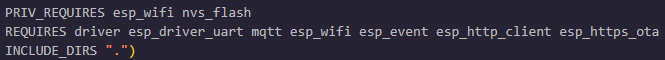
\includegraphics[width=0.9\linewidth]{Img/cmakelist_dirs.png}
    \caption{Inclusión estricta de dependencias en el archivo de construcción CMakeLists.txt.}
    \label{fig:dirs}
\end{figure}

\section{Fase de Prototipado y Simulación Inicial}

\par El desarrollo de la primera fase del sistema de transmisión comenzó con un enfoque de validación incremental, motivado principalmente por la indisponibilidad inicial de la interfaz de desarrollo física de la impresora fiscal corporativa \cite{TheFactoryHKA_iSmart_Manual}. Para mitigar este cuello de botella y asegurar el progreso del cronograma técnico, se diseñó una metodología de simulación por software que permitió emular el comportamiento del hardware de borde (\textit{Edge}) y verificar los cimientos del \textit{firmware} en un entorno controlado antes de la integración física final \cite{TheFactoryHKA_iSmart_Manual}.

\subsection{Configuración de la Comunicación Asíncrona (UART)}

\par La comunicación física inicial entre el MT-IoT y la unidad fiscal se estructuró bajo el estándar asíncrono RS-232, utilizando los parámetros serie nativos del hardware \cite{TheFactoryHKA_Manual_Protocolos}. Al no contar con el periférico real en el laboratorio, se empleó un computador personal como activo de simulación, lo que requirió la estructuración de dos entornos de prueba sucesivos:

\begin{enumerate}
    \item \textbf{Pruebas con Terminales de Datos (RealTerm):} En primera instancia, se intentó inyectar y monitorear tramas de datos binarios de forma manual. Si bien este método permitió verificar respuestas básicas al comando \textit{Enquiry} (\texttt{ENQ = 0x05h}), tal como se aprecia en la Figura \ref{fig:enq_realterm}, la herramienta resultó inviable por conflictos de codificación: la consola presentaba limitaciones para concatenar de forma determinista caracteres hexadecimales puros (como los terminadores \texttt{STX 0x02} y \texttt{ETX 0x03}) con los 129 bytes de texto ASCII requeridos para emular una respuesta válida del \texttt{Status S1} \cite{TheFactoryHKA_Manual_Protocolos}.
    
    
    \item \textbf{Simulador Dedicado en Python:} Para solventar el problema de codificación mixta, se programó un \textit{script} de automatización nativo utilizando la biblioteca \texttt{pyserial}. Este programa simuló de manera fidedigna los registros de la impresora (a 9600 bps, 8 bits, paridad par y 1 bit de parada), interceptando solicitudes seriales y estructurando dinámicamente respuestas válidas, tal como se evidencia en la máquina de estados de la Figura \ref{fig:fsm_simulador} (el listado del programa se conserva en el Apéndice \ref{apx:codigo}).
\end{enumerate}

\begin{figure}[htbp]
    \centering
    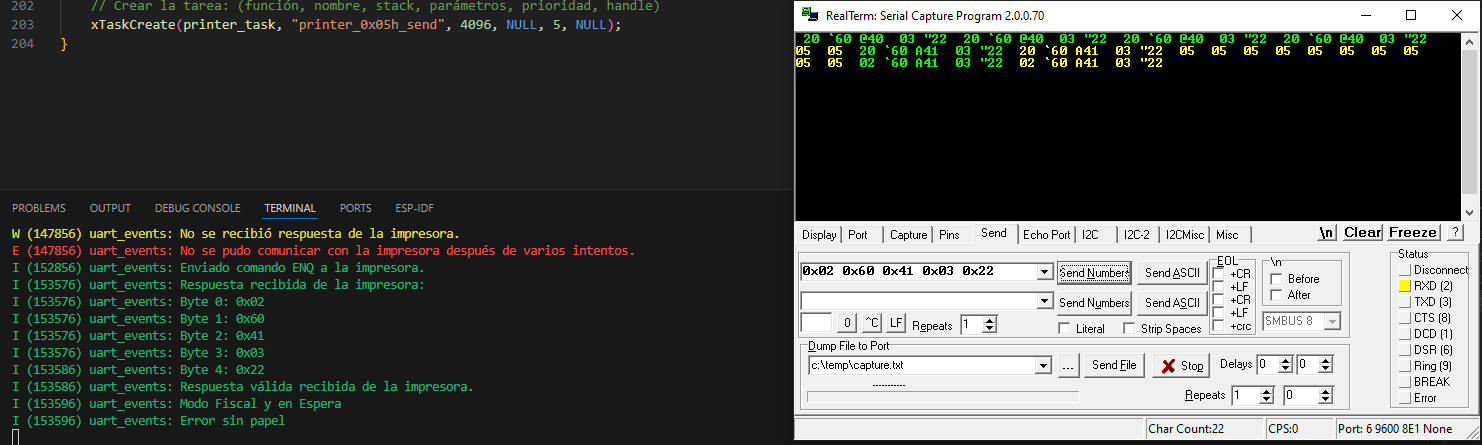
\includegraphics[width=0.95\textwidth]{Img/enq_realterm.png}
    \caption{Captura de inyección manual de tramas y comando ENQ mediante la terminal de datos RealTerm.}
    \label{fig:enq_realterm}
\end{figure}

\begin{figure}[htb]
\centering
\resizebox{0.8\textwidth}{!}{%
\begin{tikzpicture}[node distance=1.7cm, auto, >=latex',
    proc/.style={rectangle, draw, rounded corners, fill=blue!10, text width=3.4cm, align=center, minimum height=1.0cm, font=\small},
    dec/.style={diamond, draw, fill=orange!15, aspect=2.6, align=center, inner sep=1pt, font=\small},
    ar/.style={thick,->,>=stealth}]
    \node [proc] (rx) {Recepción del bloque (STX \ldots ETX)};
    \node [proc, below=of rx] (lrc) {Cálculo del LRC acumulado (XOR)};
    \node [dec, below=of lrc] (dec) {¿LRC válido?};
    \node [proc, below left=1.3cm and 1.4cm of dec] (ack) {Respuesta ACK (0x06)};
    \node [proc, below right=1.3cm and 1.4cm of dec] (nak) {Respuesta NAK (0x15)};
    \draw [ar] (rx) -- (lrc);
    \draw [ar] (lrc) -- (dec);
    \draw [ar] (dec) -- node[left, font=\scriptsize]{sí} (ack);
    \draw [ar] (dec) -- node[right, font=\scriptsize]{no} (nak);
\end{tikzpicture}%
}
\caption{Máquina de estados del simulador fiscal en software.}
\label{fig:fsm_simulador}
\end{figure}

\vspace{0.5cm}

\par En el entorno del MT-IoT, bajo el núcleo del RTOS, se implementó la tarea base denominada \texttt{printer\_polling\_task} \cite{FreeRTOS_Kernel_Ref}. El aspecto clave de esta rutina fue la sustitución de los retardos secuenciales bloqueantes por una cesión voluntaria del control al planificador (véase el Algoritmo \ref{alg:polling}) \cite{FreeRTOS_Kernel_Ref}. Al utilizar la macro \texttt{pdMS\_TO\_TICKS}, el planificador suspende la tarea durante la ventana de $5000\text{ ms}$, liberando tiempo de CPU para que el segundo núcleo procese el \textit{stack} de red sin interrupciones \cite{FreeRTOS_Kernel_Ref}.

\begin{algorithm}[htbp]
\caption{Tarea de interrogación serial no bloqueante.}
\label{alg:polling}
\begin{algorithmic}[1]
\State Inicializar la tarea de sondeo fiscal.
\While{verdadero}
    \State Transmitir el carácter de encuesta \texttt{ENQ} (0x05) por el bus local.
    \State Ceder el control al planificador durante $T_{s} = 5000$~ms.
\EndWhile
\end{algorithmic}
\end{algorithm}

\subsection{Integración de Mensajería Ligera (MQTT sobre TCP)}

\par Una vez consolidada la captura de datos locales, el desarrollo se orientó a la capa de transporte. Previo a la implementación final, se realizó una validación enviando tramas crudas mediante peticiones \texttt{HTTP GET} hacia la nube, lo que confirmó el correcto dimensionamiento del \textit{heap} para el \textit{stack} de red Wi-Fi de ESP-IDF \cite{Espressif_ESP_IDF_v552}.\\

\par Sin embargo, para cumplir con los requerimientos industriales de mínima sobrecarga (\textit{overhead}) de cabecera y envío asíncrono, se migró hacia el estándar MQTT v5.0 sobre conexiones TCP/IP \cite{OASIS_MQTT_v5}. El prototipado inicial utilizó el \textit{broker} de código abierto \textit{Eclipse Mosquitto} en el entorno local (puerto estándar 1883 no cifrado) \cite{OASIS_MQTT_v5}.\\

\par El \textit{firmware} orquestó la conexión mediante el bucle de eventos \texttt{mqtt\_event\_handler}. Al recibir la confirmación de conexión (\texttt{MQTT\_EVENT\_CONNECTED}), el sistema disparaba la tarea de publicación a través del nivel de calidad de servicio \texttt{QoS 1} (entrega garantizada al menos una vez). Las pruebas operativas se realizaron empaquetando el \texttt{Status S1} simulado en cadenas JSON planas hacia una jerarquía preliminar de tópicos, sentando las bases para el modelado asíncrono y los mecanismos de persistencia del servidor web final \cite{Django_v5_Doc}.\\

\par La efectividad de este canal de transporte se validó mediante la intercepción del \textit{payload} en el \textit{Broker} HiveMQ. Tal como se documenta en la Tabla \ref{tab:json_s1}, el microcontrolador logró empaquetar exitosamente los registros crudos de la impresora en una estructura clave-valor legible, confirmando la correcta extracción del RIF, los acumuladores de ventas y los estados operativos. El listado textual del mensaje se conserva en el Apéndice \ref{apx:codigo}.

\begin{table}[htbp]
\centering
\caption{Estructura del mensaje JSON del \texttt{Status S1} publicado hacia el \textit{broker} MQTT.}
\label{tab:json_s1}
\begin{tabularx}{\textwidth}{@{}l l >{\raggedright\arraybackslash}X@{}}
\toprule
\textbf{Clave} & \textbf{Tipo} & \textbf{Descripción} \\
\midrule
\texttt{timestamp} & Entero & Marca temporal del RTOS en milisegundos \\
\texttt{sts1} & Cadena & Estado lógico del equipo (p. ej., \texttt{0x60}) \\
\texttt{sts2} & Cadena & Estado del mecanismo de impresión (p. ej., \texttt{0x40}) \\
\texttt{estado} & Cadena & Descripción textual del estado lógico \\
\texttt{error} & Cadena & Descripción textual del error mecánico \\
\texttt{cajero} & Cadena & Identificador del cajero (ATM) \\
\texttt{ventas} & Cadena & Acumulador de ventas diarias \\
\texttt{fact\_emitidas} & Cadena & Contador de facturas emitidas \\
\texttt{rif} & Cadena & Registro de Información Fiscal del contribuyente \\
\texttt{registro} & Cadena & Número de registro de la máquina \\
\bottomrule
\end{tabularx}
\end{table}

\section{Diagnóstico e Identificación de Inestabilidades en Entornos Industriales Hostiles}

\par A medida que el \textit{firmware} del Módulo de Transmisión IoT (MT-IoT) incorporó las capas de seguridad criptográfica y la lógica de transporte hacia la nube, el sistema comenzó a exhibir cuellos de botella operativos y fallos de estabilidad. Esta sección analiza las limitaciones críticas identificadas en el hardware y el software durante las pruebas de estrés en condiciones operativas, las cuales comprometían el determinismo y la alta disponibilidad exigidas para un dispositivo industrial \cite{Connected_Everything_2016}.

\subsection{Restricciones de Memoria y Gestión de la pila IRAM}

\par La integración de una comunicación segura basada en cifrado de clave pública hacia el \textit{Broker} requirió la habilitación de la pila de seguridad Mbed TLS nativa de ESP-IDF \cite{Espressif_ESP_IDF_v552}. Sin embargo, la inicialización del \textit{handshake} TLS/SSL, la validación de certificados raíz para HiveMQ Cloud y el procesamiento dinámico de objetos mediante la librería \texttt{cJSON} generaron un consumo exponencial de memoria en el microcontrolador \cite{FreeRTOS_Kernel_Ref}.\\

\par En la arquitectura del SoC ESP32, la memoria interna SRAM de 520 KB se divide lógicamente en segmentos de instrucción (IRAM) y de datos (DRAM) \cite{Espressif_ESP32_Datasheet}. Durante las pruebas de estrés con la pila segura y el cliente de telemetría activos, el uso de la IRAM escaló críticamente hasta alcanzar el 78.39\% (102,751 Bytes utilizados de 131,072 Bytes disponibles), dejando un estrecho margen operativo, tal como se evidencia en la Figura \ref{fig:iram_crisis}.

\begin{figure}[htbp]
    \centering
    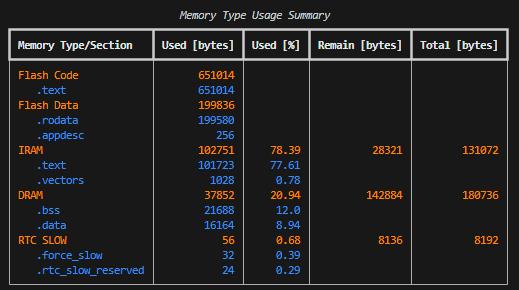
\includegraphics[width=0.75\linewidth]{Img/iram_crisis.png}
    \caption{Perfilado de memoria revelando un nivel crítico de ocupación de la IRAM (78.39\%).}
    \label{fig:iram_crisis}
\end{figure}

\par Este escenario de alta ocupación presentaba riesgos técnicos severos:

\begin{itemize}
    \item \textbf{Desbordamiento de Pila (\textit{Stack Overflow}):} El planificador de tareas de FreeRTOS quedaba vulnerable ante picos de tráfico de red o lazos de reconexión asíncronos, donde cualquier asignación de pila adicional provocaría un reinicio crítico del sistema por pánico del \textit{kernel}.
    
    \item \textbf{Inviabilidad del Sistema de Actualización (OTA):} La saturación de memoria impedía reservar el espacio dinámico (\textit{heap}) requerido para alojar los \textit{buffers} de descarga del cliente HTTP, imposibilitando la orquestación de la tabla de particiones dual (Factory + 2 OTA).
\end{itemize}

\subsection{Interferencia Electromagnética y Basura en el Bus UART}

\par En la etapa de prototipado inicial, la captura local de datos fiscales se realizaba utilizando el transceptor asíncrono UART \cite{TheFactoryHKA_Manual_Protocolos}. Al implementar el flujo bidireccional estricto gobernado por caracteres de control físicos (\texttt{ACK 0x06h} y \texttt{NAK 0x15h}), se evidenció que este estándar presentaba vulnerabilidades inaceptables para la robustez industrial.\\

\par Debido a la ausencia de blindaje electromagnético en el cable de interconexión local y la naturaleza asíncrona del bus, las líneas físicas actuaban como antenas ante el ruido y la interferencia electromagnética (EMI) del entorno. Esta inyección de ruido deformaba los bits de datos en tránsito, insertando "basura" en el controlador de hardware del microcontrolador.\\

\par Al alterarse las tramas físicas (especialmente los 129 bytes del comando \texttt{Status S1}), el \textit{firmware} fallaba en la comprobación matemática de redundancia longitudinal (LRC) \cite{TheFactoryHKA_Manual_Protocolos}. Para mitigar temporalmente este fenómeno antes de la migración definitiva a la interfaz síncrona, se implementó una estricta validación por \textit{software} que descartaba las tramas corruptas y liberaba el bus, tal como se documenta en el Algoritmo \ref{alg:lrc}.

\begin{algorithm}[htbp]
\caption{Validación de integridad de trama e intercepción de ruido electromagnético.}
\label{alg:lrc}
\begin{algorithmic}[1]
\State Recibir la trama $(STX, D, ETX, LRC_{rx})$.
\If{$STX \neq \texttt{0x02}$ \textbf{o} $ETX \neq \texttt{0x03}$}
    \State Enviar \texttt{NAK} y descartar la trama.
\EndIf
\State Calcular $LRC_{calc} \leftarrow \bigoplus_{i=1}^{n-1} b_i$.
\If{$LRC_{rx} = LRC_{calc}$}
    \State Enviar \texttt{ACK}.
\Else
    \State Enviar \texttt{NAK}, incrementar el contador de errores y liberar el bus.
\EndIf
\end{algorithmic}
\end{algorithm}

\subsection{Problemas de Concurrencia (Race Conditions)}

\par La orquestación multitarea de FreeRTOS permite ejecutar procesos de forma paralela en los dos núcleos del ESP32 \cite{FreeRTOS_Kernel_Ref}. Sin embargo, la coexistencia de la tarea de adquisición fiscal continua y la recepción de comandos inalámbricos introdujo condiciones de carrera (\textit{Race Conditions}) severas:

\begin{enumerate}
    \item \textbf{Colisiones Eléctricas (\say{Choque de Trenes}):} Durante las pruebas iniciales de actualización, si el microcontrolador recibía un comando de descarga OTA por MQTT exactamente en el mismo milisegundo en que la tarea fiscal iniciaba su ciclo de sondeo, ambas rutinas intentaban polarizar las líneas físicas locales simultáneamente. Al carecer de exclusión mutua coordinada a nivel de \textit{hardware}, el controlador entraba en pánico (lanzando una excepción \texttt{assert failed}) y forzaba el reinicio de la placa (véase la Figura \ref{fig:choque_trenes}).
    
    \item \textbf{Lecturas Cruzadas (\textit{Corrupción de RAM}):} A nivel lógico, la tarea de monitoreo sobrescribía continuamente los acumuladores de ventas en los búferes de la memoria RAM. Si la tarea MQTT despertaba de manera asíncrona para empaquetar el \textit{payload} JSON en ese preciso lapso, leía una mezcla de datos viejos y nuevos, transmitiendo telemetría fiscal híbrida y corrupta hacia el servidor.
\end{enumerate}

\begin{figure}[htbp]
\centering
\begin{tikzpicture}[>=latex',
    task/.style={rectangle, draw, rounded corners, fill=blue!10, minimum width=3.6cm, minimum height=1.1cm, align=center, font=\small},
    bus/.style={rectangle, draw, fill=orange!20, minimum width=3.2cm, minimum height=1.4cm, align=center, font=\small},
    ev/.style={rectangle, draw, fill=red!15, rounded corners, minimum width=3.6cm, minimum height=1.0cm, align=center, font=\scriptsize},
    ar/.style={thick,->,>=stealth}]
    \node [task] (poll) at (0,2.2) {Tarea \texttt{Polling}\\ (sondeo fiscal $S1$)};
    \node [task] (ota) at (0,-0.2) {Tarea \texttt{OTA}\\ (reescritura de firmware)};
    \node [bus] (bus) at (6.2,1.0) {Bus SPI local\\(pines compartidos)};
    \node [ev] (crash) at (6.2,-1.9) {\texttt{assert failed}\\reinicio del SoC};
    \draw [ar, red] (poll.east) -- node[above, font=\scriptsize, text=red]{$t_0$} (bus.west);
    \draw [ar, red] (ota.east) -- node[below, font=\scriptsize, text=red]{$t_0$} (bus.west);
    \draw [ar] (bus.south) -- (crash.north);
    \node [font=\scriptsize, text=red, align=center] at (3.1,-1.9) {acceso simultáneo\\sin mutex};
\end{tikzpicture}
\caption{Traza de depuración y registro de evento ante colisión por acceso concurrente al bus local (Choque de Trenes).}
\label{fig:choque_trenes}
\end{figure}

\par Estas limitaciones demostraron empíricamente que, para un entorno de control tributario, no basta con lograr comunicación bidireccional; es mandatorio implementar mecanismos de exclusión mutua por \textit{hardware} (como \textit{Mutexes}) y optimizaciones granulares de la memoria \cite{Espressif_ESP32_Datasheet}.

\section{Diseño de un Kernel Concurrente e Invariante de Red a Prueba de Condiciones de Carrera}

\par Una vez identificados los cuellos de botella en la gestión de memoria, la vulnerabilidad al ruido eléctrico de la línea de datos asíncrona y las condiciones de carrera en los hilos de FreeRTOS, se procedió a realizar una re-ingeniería profunda sobre los cimientos del \textit{firmware} del MT-IoT \cite{Espressif_ESP_IDF_v552}. Esta fase se enfocó en reestructurar la capa de abstracción de \textit{hardware} y optimizar el planificador de tareas de tiempo real para asegurar el determinismo y la resiliencia del sistema en entornos industriales hostiles.

\subsection{Implementación de la Interfaz Síncrona de Alto Rendimiento}

\par Para mitigar la inyección de bytes corruptos generada por la susceptibilidad electromagnética del estándar asíncrono, se migró la interconexión física local hacia una interfaz de comunicación serie síncrona dedicada, operando a una frecuencia de 100 kHz \cite{Espressif_ESP32_Datasheet}. A diferencia de la comunicación UART anterior, este método basa el muestreo de datos en una señal de temporización (\textit{Clock}) dedicada, generada por el ESP32 en rol de maestro, eliminando de raíz las desviaciones por deriva de reloj (\textit{baud-rate drift}) y garantizando una transmisión determinista \cite{Espressif_ESP_IDF_v552}. La disposición física de este enlace maestro-esclavo se ilustra en la Figura \ref{fig:bus_sincrono}.\\

\begin{figure}[htbp]
\centering
\begin{tikzpicture}[>=latex',
    box/.style={rectangle, draw, rounded corners, fill=blue!10, minimum width=2.8cm, minimum height=2.6cm, align=center, font=\small},
    lbl/.style={font=\scriptsize, inner sep=1pt}]
    \node [box] (m) {ESP32\\[3pt]\textit{Maestro}};
    \node [box, right=6.5cm of m] (s) {Periférico Fiscal\\[3pt]\textit{Esclavo}};
    \draw [->] ([yshift=20pt]m.east) -- node[above, lbl]{(reloj, 100 kHz)} ([yshift=20pt]s.west);
    \draw [->] ([yshift=7pt]m.east) -- node[above, lbl]{(habilitación del esclavo)} ([yshift=7pt]s.west);
    \draw [->] ([yshift=-7pt]m.east) -- node[below, lbl]{(datos de transmisión)} ([yshift=-7pt]s.west);
    \draw [->] ([yshift=-20pt]s.west) -- node[below, lbl]{(datos de recepción)} ([yshift=-20pt]m.east);
\end{tikzpicture}
\caption{Interacción maestro-esclavo sobre el bus síncrono local, con señal de reloj dedicada a 100 kHz y vías independientes de transmisión y recepción.}
\label{fig:bus_sincrono}
\end{figure}

\par Para blindar la integridad lógica de las tramas tributarias en esta nueva capa física, se implementó una rutina matemática de validación de redundancia longitudinal (LRC). Tras recibir cada bloque de datos, el \textit{firmware} ejecuta un lazo cerrado que realiza operaciones lógicas \texttt{XOR} acumulativas sobre los bytes recibidos, contrastando el resultado con el \textit{checksum} enviado por el periférico fiscal \cite{TheFactoryHKA_Manual_Protocolos}.\\

\par Si la trama es declarada válida, el MT-IoT responde con un carácter \texttt{ACK (0x06h)}; de lo contrario, envía un \texttt{NAK (0x15h)} y procede de inmediato a reiniciar lógicamente los registros del hardware del bus local, impidiendo la propagación de datos corruptos en la memoria del sistema.\\

\par Adicionalmente, para evitar bloqueos del procesador si el periférico es apagado físicamente, se establecieron temporizadores (\textit{timeouts}) estrictos. Si se supera el límite de fallos continuos, el \textit{firmware} transiciona al estado de pánico y activa una máquina de reconexión, sin bloquear las tareas de red \cite{FreeRTOS_Kernel_Ref}.

\subsection{Orquestación Concurrente mediante FreeRTOS}

\par El control cooperativo del MT-IoT se organizó bajo el \textit{kernel} de FreeRTOS mediante un esquema de exclusión mutua de dos niveles, solventando la condición de carrera identificada en la etapa de prototipado:

\begin{enumerate}
    \item \textbf{Exclusión Mutua de Datos en RAM (\texttt{mqtt\_data\_mutex}):} Se implementó un semáforo tipo \textit{Mutex} para proteger la estructura \texttt{mqtt\_data\_t} en la DRAM. Este candado lógico garantiza que la tarea de monitoreo local no pueda sobrescribir variables de facturación mientras la tarea MQTT está leyendo el bloque para formatear el \textit{payload} JSON, evitando el tránsito de datos híbridos.
    
    \item \textbf{Exclusión Mutua del Bus Físico (\texttt{bus\_local\_mutex}):} Para resolver la colisión eléctrica local (choque de trenes) cuando una actualización remota coincide con el sondeo periódico de 5 segundos, se introdujo un segundo \textit{Mutex} de \textit{hardware}. Como se observa en la Figura \ref{fig:mutex_doble}, tanto la tarea de sondeo como la rutina OTA deben competir y adquirir con éxito este semáforo antes de poder energizar el canal de comunicación físico. El listado de la implementación se conserva en el Apéndice \ref{apx:codigo}.
\end{enumerate}

\begin{figure}[htb]
\centering
\begin{tikzpicture}[node distance=1.3cm, auto, >=latex',
    proc/.style={rectangle, draw, rounded corners, fill=blue!10, text width=6cm, align=center, minimum height=1.0cm, font=\small},
    dec/.style={diamond, draw, fill=orange!15, aspect=3.2, align=center, inner sep=1pt, font=\small},
    ar/.style={thick,->,>=stealth}]
    \node [proc] (ini) {Solicitud de acceso al bus local};
    \node [dec, below=of ini] (m1) {¿Mutex del bus?};
    \node [proc, below=of m1] (val) {Validación de la trama (LRC)};
    \node [dec, below=of val] (m2) {¿Mutex de datos?};
    \node [proc, below=of m2] (wr) {Escritura en la estructura de telemetría};
    \node [proc, below=of wr] (rel) {Liberación de ambos semáforos};
    \draw [ar] (ini) -- (m1);
    \draw [ar] (m1) -- node[right, font=\scriptsize]{sí} (val);
    \draw [ar] (val) -- (m2);
    \draw [ar] (m2) -- node[right, font=\scriptsize]{sí} (wr);
    \draw [ar] (wr) -- (rel);
\end{tikzpicture}
\caption{Exclusión mutua en dos niveles para la protección de la memoria RAM y del bus físico.}
\label{fig:mutex_doble}
\end{figure}

\par Para proteger la memoria (\textit{heap}) ante ráfagas de comandos MQTT, la lógica OTA se desacopló del bucle principal. Se creó la tarea \texttt{ota\_supervisor\_task}. Al detectarse un comando de actualización, el manejador MQTT empuja la solicitud a una cola segura (\texttt{ota\_cmd\_queue}). Al despertar, el supervisor activa una bandera global de \say{freno de mano} (\texttt{ota\_en\_progreso = true}) que paraliza la tarea fiscal, y ejecuta la descarga en total aislamiento \cite{Espressif_ESP_IDF_v552}.

\subsection{Estrategias de Resiliencia de Red y DNS Injection}

\par Para cumplir con los requerimientos de robustez industrial, el \textit{firmware} se dotó de mecanismos de autodefensa. Ante cortes del proveedor de internet (ISP), la capa de red del microcontrolador gatilla asíncronamente el evento \texttt{WIFI\_EVENT\_STA\_DISCONNECTED}, iniciando un lazo de reconexión infinito que intenta reanudar el enlace sin reiniciar la lógica de control interna \cite{Espressif_ESP_IDF_v552}.\\

\par Uno de los aportes más significativos fue la mitigación de fallos de resolución de nombres (\textit{DNS}) del contribuyente. Al capturar una dirección IP local a través del evento \texttt{IP\_EVENT\_STA\_GOT\_IP}, la pasarela intercepta dinámicamente la configuración de la interfaz de red (\textit{netif}) e inyecta forzosamente los servidores principales de Google (8.8.8.8) \cite{Espressif_ESP_IDF_v552}. Esta técnica asegura que el cliente TLS siempre resuelva la ruta hacia HiveMQ.\\

\par Finalmente, ante caídas temporales del servidor MQTT, el \textit{firmware} impone un retardo de cortesía (\texttt{RECONNECT\_DELAY\_MS}) antes de intentar levantar el \textit{socket} nuevamente (véase el Algoritmo \ref{alg:reconexion}). Esto evita ataques de denegación de servicio (DDoS) involuntarios contra el \textit{Broker} y estabiliza el consumo energético del MT-IoT.

\begin{algorithm}[htbp]
\caption{Resiliencia y reconexión no bloqueante en la tarea MQTT.}
\label{alg:reconexion}
\begin{algorithmic}[1]
\While{verdadero}
    \State Esperar la notificación de un evento de la pila de red.
    \If{la conexión con el \textit{broker} no está activa}
        \State Aplicar un retardo de cortesía $T_{r} = \texttt{RECONNECT\_DELAY\_MS}$.
        \State Continuar el ciclo sin descartar la telemetría pendiente.
    \EndIf
    \State Publicar la telemetría retenida.
\EndWhile
\end{algorithmic}
\end{algorithm}

\section{Protocolo de Comunicación Segura y Mensajería MQTT v5.0}

\par Una vez consolidada la estabilidad del \textit{firmware} en su capa de adquisición local y resueltos los conflictos de concurrencia multitarea, el desarrollo se enfocó en el establecimiento de un canal de telemetría de grado industrial hacia la nube \cite{Connected_Everything_2016}. La implementación de la pila de red se diseñó bajo el estándar MQTT v5.0, operando sobre conexiones TCP/IP persistentes hacia la infraestructura de HiveMQ Cloud \cite{OASIS_MQTT_v5}. Este diseño satisface tanto los requerimientos de mínima sobrecarga de red (\textit{overhead}) como la exigencia innegociable de garantizar la confidencialidad de la información fiscal en tránsito.

\subsection{Seguridad en la Capa de Transporte (TLS/SSL)}

\par El transporte de información tributaria sensible a través de internet requiere esquemas de cifrado robustos que impidan ataques de interceptación pasiva (\textit{eavesdropping}) o inyección de contenido. Para cumplir con esta directiva, el cliente MQTT embebido en el ESP32 se configuró para establecer \textit{sockets} seguros utilizando el protocolo TLS v1.2, apoyado en la biblioteca Mbed TLS nativa de ESP-IDF \cite{Espressif_ESP_IDF_v552}.\\

\par La orquestación de la seguridad se estructuró dentro de la estructura de configuración del cliente (\texttt{esp\_mqtt\_client\_config\_t}), aplicando dos decisiones de diseño fundamentales que se evidencian en la Tabla \ref{tab:tls_config}:

\begin{enumerate}
    \item \textbf{Puerto Seguro y Cifrado por Hardware:} Se forzó el enrutamiento hacia el puerto estándar 8883 (\texttt{secure-mqtt}), estableciendo el transporte como \texttt{MQTT\_TRANSPORT\_OVER\_SSL}. Esto obliga al microcontrolador a realizar un \textit{Handshake} criptográfico, negociando algoritmos de cifrado simétrico mediante la aceleración por \textit{hardware} integrada en el silicio del SoC \cite{Espressif_ESP32_Datasheet}.
    
    \item \textbf{Autenticación mediante \textit{Bundle} de Certificados:} Para mitigar ataques de intermediario (\textit{Man-in-the-Middle}), el MT-IoT verifica la cadena de confianza de HiveMQ Cloud. En lugar de quemar estáticamente extensos archivos PEM en la Flash (lo que degradaría la memoria), se habilitó el parámetro \texttt{crt\_bundle\_attach}. Esta técnica enlaza un catálogo optimizado de Autoridades de Certificación (CAs) confiables provisto por Espressif, logrando una validación robusta con un consumo residual de almacenamiento \cite{Espressif_ESP_IDF_v552}.
\end{enumerate}

\begin{table}[htbp]
\centering
\caption{Parámetros de configuración del cliente MQTT con seguridad TLS estricta.}
\label{tab:tls_config}
\begin{tabularx}{\textwidth}{@{}l >{\raggedright\arraybackslash}X@{}}
\toprule
\textbf{Parámetro} & \textbf{Valor o función} \\
\midrule
\texttt{broker.address.hostname} & Dominio del \textit{broker} HiveMQ Cloud \\
\texttt{broker.address.port} & 8883 (\texttt{secure-mqtt}) \\
\texttt{broker.address.transport} & \texttt{MQTT\_TRANSPORT\_OVER\_SSL} \\
\texttt{broker.verification.crt\_bundle\_attach} & \texttt{esp\_crt\_bundle\_attach} (validación de CAs) \\
\texttt{session.protocol\_ver} & \texttt{MQTT\_PROTOCOL\_V\_5} \\
\bottomrule
\end{tabularx}
\end{table}

\par En el extremo del servidor, el \textit{worker} asíncrono de Django se configuró de manera homóloga para forzar el protocolo TLS v1.2, garantizando un ecosistema cerrado de extremo a extremo. Adicionalmente, el formateo del \textit{payload} en C se implementó utilizando exclusivamente la función \texttt{snprintf} para delimitar rígidamente las cadenas de caracteres, previniendo desbordamientos de búfer (\textit{Buffer Overflows}) y protegiendo el \textit{stack} de la tarea de red.

\subsection{Trazabilidad mediante User Properties y Last Will and Testament}

\par La adopción del estándar MQTT v5.0 permitió incorporar capacidades avanzadas de diagnóstico que no eran viables en versiones anteriores (v3.1.1) \cite{OASIS_MQTT_v5}. El \textit{firmware} explota estas características para optimizar la trazabilidad y la resiliencia del monitoreo en tiempo real.\\

\par En primer lugar, se implementó el uso de \textit{User Properties} en cada paquete de publicación (\texttt{PUBLISH}). Estas propiedades actúan como metadatos en formato clave-valor (UTF-8) anidados en la cabecera del protocolo de red, permitiendo su lectura por el servidor web sin necesidad de ejecutar rutinas costosas de deserialización sobre el \textit{payload} JSON principal \cite{OASIS_MQTT_v5}. Tal como se documenta en la Tabla \ref{tab:user_props}, el \textit{firmware} inyecta dinámicamente propiedades críticas como el RSSI (intensidad de señal Wi-Fi) y el número de serie.

\begin{table}[htbp]
\centering
\caption{Propiedades de usuario (\textit{User Properties}) inyectadas en cada publicación MQTT v5.0.}
\label{tab:user_props}
\begin{tabularx}{\textwidth}{@{}l >{\raggedright\arraybackslash}X@{}}
\toprule
\textbf{Clave} & \textbf{Contenido} \\
\midrule
\texttt{modelo\_dispositivo} & Modelo del equipo (\texttt{HKA80}) \\
\texttt{firmware\_version} & Versión del firmware del MT-IoT \\
\texttt{serial} & Número de serie del periférico \\
\texttt{tipo\_dato} & Clasificación del mensaje (\texttt{status\_s1}) \\
\texttt{wifi\_rssi} & Intensidad de señal Wi-Fi en dBm \\
\bottomrule
\end{tabularx}
\end{table}

\par En segundo lugar, para resolver la imposibilidad de realizar un sondeo constante (\textit{polling}) desde el servidor web hacia miles de clientes, se configuró el mecanismo \textit{Last Will and Testament} (LWT) o Testamento de MQTT \cite{OASIS_MQTT_v5}. Durante el establecimiento de la sesión con el \textit{Broker}, el MT-IoT registra una \say{última voluntad} con un nivel de calidad \texttt{QoS 1} y la bandera de retención (\textit{Retain Flag}) activa. El \textit{payload} preconfigurado declara el estado \texttt{offline} y la alerta \texttt{conexion\_perdida\_abruptamente}; su contenido textual exacto se conserva en el Apéndice \ref{apx:codigo}.\\

\par Si el MT-IoT experimenta una pérdida abrupta de energía o falla de red, el \textit{Broker} detecta la caída del \textit{Keep-Alive} y publica el testamento automáticamente. Al interceptar este evento, el \textit{backend} en Django ejecuta una rutina de autodefensa que congela la última lectura fiscal válida en la base de datos y emite una alerta visual, garantizando la supervisión total sin sobrecargar la red.

\section{Arquitectura de Puente Síncrono de Reescritura Remota para Periféricos In Situ (OTA Doble Objetivo)}

\par Uno de los requerimientos no funcionales más exigentes es la capacidad de mantener el ciclo de vida del \textit{hardware} en campo sin requerir la intervención física de soporte técnico \cite{WEF_IIoT_2018}. Para superar este desafío operativo, se diseñó un protocolo de Actualización Inalámbrica (OTA, \textit{Over-The-Air}) de doble objetivo. Este sistema inédito en la arquitectura de la empresa permite canalizar, a través del túnel seguro MQTT, comandos de bajo nivel para reescribir tanto el \textit{firmware} del MT-IoT como el código interno del periférico fiscal.\\

\par El flujo inicia en la interfaz de gestión web, donde el administrador selecciona el archivo binario compilado (\texttt{.bin}). El servidor publica un \textit{payload} JSON estructurado en el tópico de comandos de actualización del dispositivo \cite{OASIS_MQTT_v5}. Tal como se aprecia en la Tabla \ref{tab:json_ota}, este paquete define la instrucción, el \textit{hardware} de destino (MT-IoT o Impresora), la versión esperada y una ruta segura de descarga de un solo uso. El listado textual del mensaje se conserva en el Apéndice \ref{apx:codigo}.

\begin{table}[htbp]
\centering
\caption{Estructura del mensaje JSON de comando para iniciar una actualización remota.}
\label{tab:json_ota}
\begin{tabularx}{\textwidth}{@{}l l >{\raggedright\arraybackslash}X@{}}
\toprule
\textbf{Campo} & \textbf{Ejemplo} & \textbf{Función} \\
\midrule
\texttt{comando} & \texttt{INICIAR\_OTA} & Instrucción de actualización \\
\texttt{objetivo} & \texttt{ismart} / \texttt{printer} & Hardware de destino \\
\texttt{version} & \texttt{v020100} & Versión esperada del firmware \\
\texttt{url\_descarga} & Ruta del binario & Dirección segura de descarga \\
\bottomrule
\end{tabularx}
\end{table}

\subsection{Actualización del Módulo Gateway (ESP32)}

\par Cuando el MT-IoT intercepta el comando y valida que el campo \texttt{objetivo} equivale a \say{\texttt{ismart}}, el \textit{firmware} activa el estado global \texttt{ota\_en\_progreso = true}. Este indicador lógico actúa como un "freno de mano" que suspende inmediatamente el ciclo de sondeo fiscal de 5 segundos, aislando el bus de datos local y garantizando que el microcontrolador asigne la totalidad de sus recursos de memoria RAM al procesamiento de la descarga.\\

\par El proceso de autoactualización se fundamenta en la API \texttt{esp\_https\_ota} nativa de Espressif \cite{Espressif_ESP_IDF_v552}. Para viabilizar este mecanismo de forma segura, se parametrizó la memoria del \textit{hardware} bajo tres directivas estrictas \cite{Espressif_Menuconfig}:

\begin{enumerate}
    \item \textbf{Verificación Criptográfica (\textit{Bundle}):} La tarea de descarga utiliza el sistema \texttt{esp\_crt\_bundle\_attach} para verificar asíncronamente la identidad del servidor de medios, blindando al dispositivo contra la inyección de código malicioso no firmado.
    
    \item \textbf{Resiliencia mediante Doble Partición:} En el mapa de memoria se configuró una tabla de particiones del tipo \say{\textbf{Factory app, two OTA definitions}}. Esto divide la Flash de 4 MB en regiones idénticas (OTA\_0 y OTA\_1). El \textit{firmware} reescribe progresivamente la partición inactiva; si ocurre un corte de energía, el sistema descarta el sector corrupto y arranca desde la partición actual intacta \cite{Espressif_ESP_IDF_v552}.
\end{enumerate}

\par Al culminar exitosamente la descarga, el MT-IoT invoca una rutina de limpieza que desinicializa la interfaz local, corta las conexiones de red y ejecuta un reinicio por \textit{software} (\texttt{esp\_restart()}), permitiendo al \textit{Bootloader} arrancar desde el nuevo sector de memoria.

\subsection{Actualización del Firmware del Periférico Fiscal a través de la Interfaz Síncrona Local}

\par El escenario de máxima complejidad ocurre cuando el campo \texttt{objetivo} equivale a \say{\texttt{printer}}. Dado que la unidad de control fiscal carece de pila de red nativa, el MT-IoT no reescribe su propia memoria, sino que asume el rol de \textit{Host} de programación intermedio \cite{TheFactoryHKA_Manual_Protocolos}.\\

\par El proceso de actualización se divide en dos etapas asíncronas concurrentes, diseñadas para superar las severas restricciones de memoria del microcontrolador. Dado que el binario del periférico supera ampliamente la capacidad del \textit{Heap} libre del ESP32, la descarga de red no se almacena en su totalidad, sino que se procesa a través de un \textbf{búfer circular de transmisión de 1024 bytes}.\\

\par Para proteger este flujo continuo de los cortes intermitentes típicos de las redes Wi-Fi comerciales, se implementó un mecanismo de persistencia basado en la cabecera HTTP \texttt{Range} (véase el Algoritmo \ref{alg:http_range}). Si el enlace titubea, el \textit{firmware} inyecta el número exacto de bytes ya recibidos, obligando al servidor web a reanudar la transmisión desde el punto de falla, evitando descartar el progreso.\\

\begin{algorithm}[htbp]
\caption{Reanudación de descargas interrumpidas mediante cabeceras HTTP Range.}
\label{alg:http_range}
\begin{algorithmic}[1]
\State Inicializar el contador de bytes recibidos $B \leftarrow 0$.
\While{la descarga no esté completa}
    \If{$B > 0$}
        \State Fijar la cabecera \texttt{Range: bytes=}$B$\texttt{-}.
    \EndIf
    \State Abrir la conexión HTTP y solicitar el recurso.
    \State Leer los fragmentos y actualizar $B$.
\EndWhile
\end{algorithmic}
\end{algorithm}

\par A medida que el búfer se alimenta de la red, el MT-IoT orquesta la retransmisión hacia el periférico mediante el bus físico síncrono local. Este puente de datos opera bajo una estricta máquina de estados de tres fases para salvaguardar la integridad de la memoria tributaria:

\begin{enumerate}
    \item \textbf{Fase de Inicialización (\textit{Handshake}):} El MT-IoT transmite un comando de control de inicio de programación (\texttt{0x01}). El periférico, tras validar que no posee comprobantes fiscales abiertos, responde con un carácter \texttt{ACK (0x06h)}, abriendo su canal de escucha de memoria \cite{TheFactoryHKA_Manual_Protocolos}.
    
    \item \textbf{Transmisión Segmentada y Comprobación de Integridad:} Como se observa en la Figura \ref{fig:empaquetado_ota}, cada fragmento de 1024 bytes se empaqueta en una trama estructurada con cabecera de longitud, datos y un byte de verificación de redundancia (\textit{Checksum}). Si el periférico valida la redundancia localmente, emite un \texttt{ACK}, habilitando al MT-IoT a continuar. Ante un \texttt{NAK}, se admite un máximo de tres reintentos físicos antes de abortar de forma segura \cite{TheFactoryHKA_Manual_Protocolos}.
    
    \item \textbf{Fase de Integración:} Tras el último bloque, se transmite la señal de cierre (\texttt{0x07}). La impresora fiscal verifica la integridad total de su Flash interna y efectúa un reinicio por \textit{hardware}, asimilando el nuevo núcleo lógico \cite{TheFactoryHKA_Manual_Protocolos}.
\end{enumerate}

\begin{figure}[htbp]
\centering
\resizebox{0.98\textwidth}{!}{%
\begin{tikzpicture}[node distance=0.25cm, auto, >=latex',
    fld/.style={rectangle, draw, fill=blue!10, minimum height=1.1cm, minimum width=2.1cm, align=center, font=\small}]
    \node [fld] (c) {Comando\\\texttt{CMD\_PACKET}};
    \node [fld, right=of c] (np) {N.º de\\paquete};
    \node [fld, right=of np] (tp) {Total de\\paquetes};
    \node [fld, right=of tp] (ln) {Longitud\\(16 bits)};
    \node [fld, right=of ln] (d) {Datos\\(hasta 1024 B)};
    \node [fld, right=of d] (ck) {Checksum\\(XOR)};
\end{tikzpicture}%
}
\caption{Estructura de empaquetado de un fragmento de firmware hacia el periférico local.}
\label{fig:empaquetado_ota}
\end{figure}

\subsection{Máquina de Estados Finita para el Puente Síncrono Local}

 Para solventar la limitación de memoria RAM del microcontrolador al recibir un binario de gran tamaño destinado al periférico fiscal, el dispositivo actúa como un host/bridge intermedio. La reescritura de la memoria Flash remota se gobierna mediante una Máquina de Estados Finita (FSM) de tres fases con búfer circular e inyección de cabeceras HTTP Range para resiliencia ante cortes de red, cuyo comportamiento se representa en la Figura \ref{fig:fsm_ota_bridge}:

\begin{figure}[htbp]
\centering
\resizebox{\textwidth}{!}{%
\begin{tikzpicture}[node distance=2.0cm and 2.6cm, auto, >=latex',
    state/.style={rectangle, draw, fill=blue!10, text width=3.2cm, text centered, rounded corners, minimum height=1.3cm, font=\small},
    arrow/.style={thick,->,>=stealth}]

    % Nodos
    \node [state] (idle) {1. Reposo / Polling Suspendido};
    \node [state, right=of idle] (download) {2. Descarga HTTP Range (Búfer 1024B)};
    \node [state, right=of download] (flash) {3. Transmisión Síncrona Chunk/ACK};
    \node [state, below=2.0cm of flash] (commit) {4. Cierre (0x07) y Reset Periférico};

    % Conexiones Principales
    \draw[arrow] (idle) -- node[above, font=\scriptsize\bfseries] {Cmd OTA} (download);
    \draw[arrow] (download) -- node[above, font=\scriptsize\bfseries] {Búfer lleno} (flash);
    \draw[arrow] (flash) -- node[right, font=\scriptsize\bfseries] {Último bloque} (commit);
    
    % Bucle 1: Fallo de Red y Reintento por HTTP Range (Abajo del Nodo 2)
    \draw[arrow] (download.south east) .. controls +(down:1.8cm) and +(down:1.8cm) .. 
        node[below=2pt, font=\scriptsize, text width=3.0cm, align=center] {Fallo Red $\rightarrow$ Inyección HTTP Range} 
        (download.south west);

    % Bucle 2: NAK / Reintento Chunk (Arriba del Nodo 3)
    \draw[arrow] (flash.north east) .. controls +(up:1.8cm) and +(up:1.8cm) .. 
        node[above=2pt, font=\scriptsize, text width=2.8cm, align=center] {NAK $\rightarrow$ Reintento Chunk} 
        (flash.north west);

\end{tikzpicture}%
}
\caption{Máquina de estados del bridge síncrono para reprogramación de periféricos locales.}
\label{fig:fsm_ota_bridge}
\end{figure}

\section{Ecosistema Web de Gestión y Visualización}

\par Para completar la arquitectura de tres niveles del sistema de transmisión, se diseñó e implementó una plataforma de visualización, administración y orquestación centralizada en la nube \cite{Connected_Everything_2016}. El desarrollo de este ecosistema responde a la necesidad de supervisar activamente el estado operativo del parque de impresoras fiscales instaladas, registrar transiciones de estado tributario de manera histórica y comandar procesos inalámbricos asíncronos de actualización de \textit{firmware} (OTA) con estrictas garantías de autenticación y disponibilidad \cite{WEF_IIoT_2018}.

\subsection{Arquitectura del Backend: Worker MQTT Independiente}

\par El núcleo lógico que procesa el flujo masivo de telemetría entrante y sirve de enlace bidireccional con el sistema de persistencia se orquestó mediante un \textit{Worker} MQTT independiente denominado \texttt{listen\_mqtt.py}. En lugar de acoplar de forma síncrona el receptor de red al servidor web principal de Django (lo que bloquearía el manejo de solicitudes HTTP convencionales ante ráfagas de datos), se desarrolló un comando de gestión personalizado (\textit{Management Command}) \cite{Django_v5_Doc}. \\

\par Este \textit{script} opera en segundo plano mediante un lazo infinito no bloqueante 

\noindent (\texttt{client.loop\_forever()}). Como se aprecia en el Algoritmo \ref{alg:worker_mqtt}, el programa utiliza la biblioteca Paho MQTT y establece \textit{sockets} seguros mediante la librería \texttt{ssl}, forzando una sesión TLS v1.2 sobre el puerto 8883 hacia HiveMQ Cloud.

\begin{algorithm}[htbp]
\caption{Lógica de recepción, trazabilidad y manejo del testamento (LWT) en el \textit{worker} MQTT.}
\label{alg:worker_mqtt}
\begin{algorithmic}[1]
\State Al recibir un mensaje: extraer el serial y el tipo desde el tópico.
\State Decodificar el \textit{payload} JSON y sanear los caracteres de control.
\If{el tipo es \texttt{alertas\_conexion} y el estado es \texttt{offline}}
    \State Recuperar el último estado válido del dispositivo.
    \State Registrar transaccionalmente el evento \say{Desconexión Abrupta (LWT)}.
\EndIf
\end{algorithmic}
\end{algorithm}

\par La lógica analítica (\texttt{on\_message}) procesa la telemetría \texttt{Status S1} ejecutando un algoritmo de comparación contra el último registro histórico guardado en la base de datos. Si se detecta un cambio térmico, mecánico o lógico (ej., la transición de un estado limpio \texttt{0x40} a un error de fin de papel \texttt{0x41}), el \textit{backend} registra selectivamente un log independiente clasificado como \say{Cambio de Estado}, garantizando un rastreo exhaustivo libre de redundancias.

\subsection{Persistencia de Datos en SQLite y Lógica de Registro de Logs}

\par Para la persistencia del modelo relacional se seleccionó el motor SQLite (\texttt{db.sqlite3}), plenamente integrado en el ORM de Django \cite{Django_v5_Doc}. La arquitectura lógica de las tablas se estructuró de forma modular en \texttt{models.py}:

\begin{itemize} 
    \item \textbf{\texttt{Grupo} y \texttt{ModeloEquipo}:} Categorizan jerárquicamente los nodos IoT según sucursal y marca. 
    \item \textbf{\texttt{VersionFirmware}:} Almacena las rutas de los archivos binarios compilados (\texttt{.bin}). Clasifica el destino lógico bajo los identificadores de código \say{\texttt{ismart}} (para el MT-IoT) o \say{\texttt{impresora}}.
    \item \textbf{\texttt{Dispositivo}:} Entidad central validada mediante expresiones regulares para asegurar un serial exacto de diez caracteres alfanuméricos (ej. \texttt{Z1F9999988}).
    \item \textbf{\texttt{LogDispositivo}:} Tabla de auditoría vinculada al dispositivo principal.
\end{itemize}

\par Para salvaguardar la consistencia estructural, se configuró el comportamiento de eliminación en cascada (\texttt{on\_delete=models.CASCADE}). Si un administrador purga un dispositivo, todas sus dependencias (históricos y binarios) se borran transaccionalmente del disco en un solo ciclo, impidiendo registros huérfanos \cite{Django_v5_Doc}.\\

\par Adicionalmente, para combatir la inflación de almacenamiento producto del sondeo de 5 segundos, se implementó una \textbf{Lógica de Depuración Automática}. El \textit{Worker} calcula proactivamente una ventana límite de 90 días ($\texttt{fecha\_limite} = \texttt{timezone.now()} - \texttt{timedelta(days=90)}$). Todo log cuya estampa de tiempo resulte menor es purgado asíncronamente. Este mecanismo garantiza que la indexación se mantenga ultrarrápida y el tamaño del archivo en disco permanezca estable.

\subsection{Interfaz Reactiva SPA mediante Django y HTMX}

\par Inicialmente, se evaluó la extensión \textit{Django Channels} para empujar telemetría por WebSockets. Sin embargo, mantener un servidor intermedio introducía una sobrecarga crítica y complejidad en el \textit{firewall}. Para simplificar la arquitectura, se aplicó un enfoque directo: dado que HiveMQ expone un canal de WebSockets operando con cifrado sobre el puerto 8884 (WSS), se integró el cliente MQTT de JavaScript directamente en el navegador \cite{OASIS_MQTT_v5}. Esto permite a la interfaz atravesar cortafuegos corporativos y recibir telemetría fiscal en tiempo real sin intermediarios pesados.\\

\par Para proveer a la plataforma con la fluidez de una \textit{Single Page Application} (SPA) reduciendo el consumo de memoria en el cliente, se integró el \textit{framework} asíncrono ligero HTMX \cite{HTMX_Doc}. HTMX permite realizar peticiones AJAX silenciosas, intercambiando dinámicamente (\textit{swapping}) solo fragmentos del DOM sin recargar la página.\\

\par La innovación arquitectónica reside en la \textbf{Integración de Eventos Personalizados (JS-HTMX)}. Cuando el monitor MQTT.js detecta un cambio crítico (ej., avance de la OTA o alerta LWT), despacha un evento DOM hacia el navegador (\texttt{mqttNuevoLog}). La vista HTMX, cuyo flujo se representa en la Figura \ref{fig:flujo_htmx}, intercepta este evento desde el cuerpo del documento y gatilla un ciclo de refresco HTTP parcial, renderizando las nuevas filas de auditoría instantáneamente.\\

\begin{figure}[H]
\centering
\resizebox{0.95\textwidth}{!}{%
\begin{tikzpicture}[node distance=1.6cm, auto, >=latex',
    proc/.style={rectangle, draw, rounded corners, fill=blue!10, text width=3.4cm, align=center, minimum height=1.0cm, font=\small},
    ar/.style={thick,->,>=stealth}]
    \node [proc] (mqtt) {El cliente MQTT.js detecta un cambio};
    \node [proc, right=of mqtt] (ev) {Despacho del evento DOM \texttt{mqttNuevoLog}};
    \node [proc, right=of ev] (hx) {El atributo \texttt{hx-trigger} intercepta el evento};
    \node [proc, below=1.4cm of hx] (req) {Petición HTTP parcial a \texttt{/log\_capture}};
    \node [proc, below=1.4cm of ev] (swap) {Intercambio parcial del DOM};
    \draw [ar] (mqtt) -- (ev);
    \draw [ar] (ev) -- (hx);
    \draw [ar] (hx) -- (req);
    \draw [ar] (req) -- (swap);
\end{tikzpicture}%
}
\caption{Flujo de actualización reactiva del DOM mediante eventos MQTT y atributos HTMX.}
\label{fig:flujo_htmx}
\end{figure}

\par Esta hibridación tecnológica consolida un ecosistema de visualización reactivo, de bajísima latencia y altamente escalable para el entorno corporativo de monitoreo industrial.
    \chapter{Resultados}

\par En el presente capítulo se presentan y discuten los resultados cuantitativos y cualitativos obtenidos tras la integración de la arquitectura Módulo de Transmisión IoT (MT-IoT), la capa de red segura bajo el estándar MQTT v5.0 \cite{OASIS_MQTT_v5} y el ecosistema web centralizado \cite{Django_v5_Doc}. Se evalúa el desempeño del sistema ante pruebas de laboratorio y condiciones de estrés, analizando el impacto de las decisiones de ingeniería sobre el uso de recursos del microcontrolador, la latencia de transmisión y la resiliencia en entornos industriales \cite{Connected_Everything_2016}.

\section{Implementación del Prototipo Funcional de Borde}

\par La integración física de la tarjeta de desarrollo ESP32 DevKitC V4 \cite{Espressif_ESP32_Datasheet} con la unidad de control fiscal HKA80 \cite{TheFactoryHKA_Manual_Protocolos} culminó en la consolidación del prototipo funcional MT-IoT. Se verificó empíricamente la efectividad de la reasignación de la matriz de señales (IO MUX) hacia los pines libres GPIO 18 (TX) y GPIO 19 (RX) para la etapa asíncrona inicial, así como la posterior transición hacia el bus síncrono local. Esta disposición aisló eléctricamente la comunicación serial de las líneas del bus vinculadas a la memoria Flash interna del SoC \cite{Espressif_ESP32_Datasheet}, eliminando los reinicios continuos (\textit{bootloops}) documentados en la fase de diseño.\\

\par El prototipo desplegado en el entorno de pruebas (véase la Figura \ref{fig:prototipo_funcional}) demostró capacidad de respuesta operativa continua sostenida, validando las etapas de conversión de niveles de voltaje y el aislamiento galvánico de la interfaz de comunicación.

\begin{figure}[H]
    \centering
    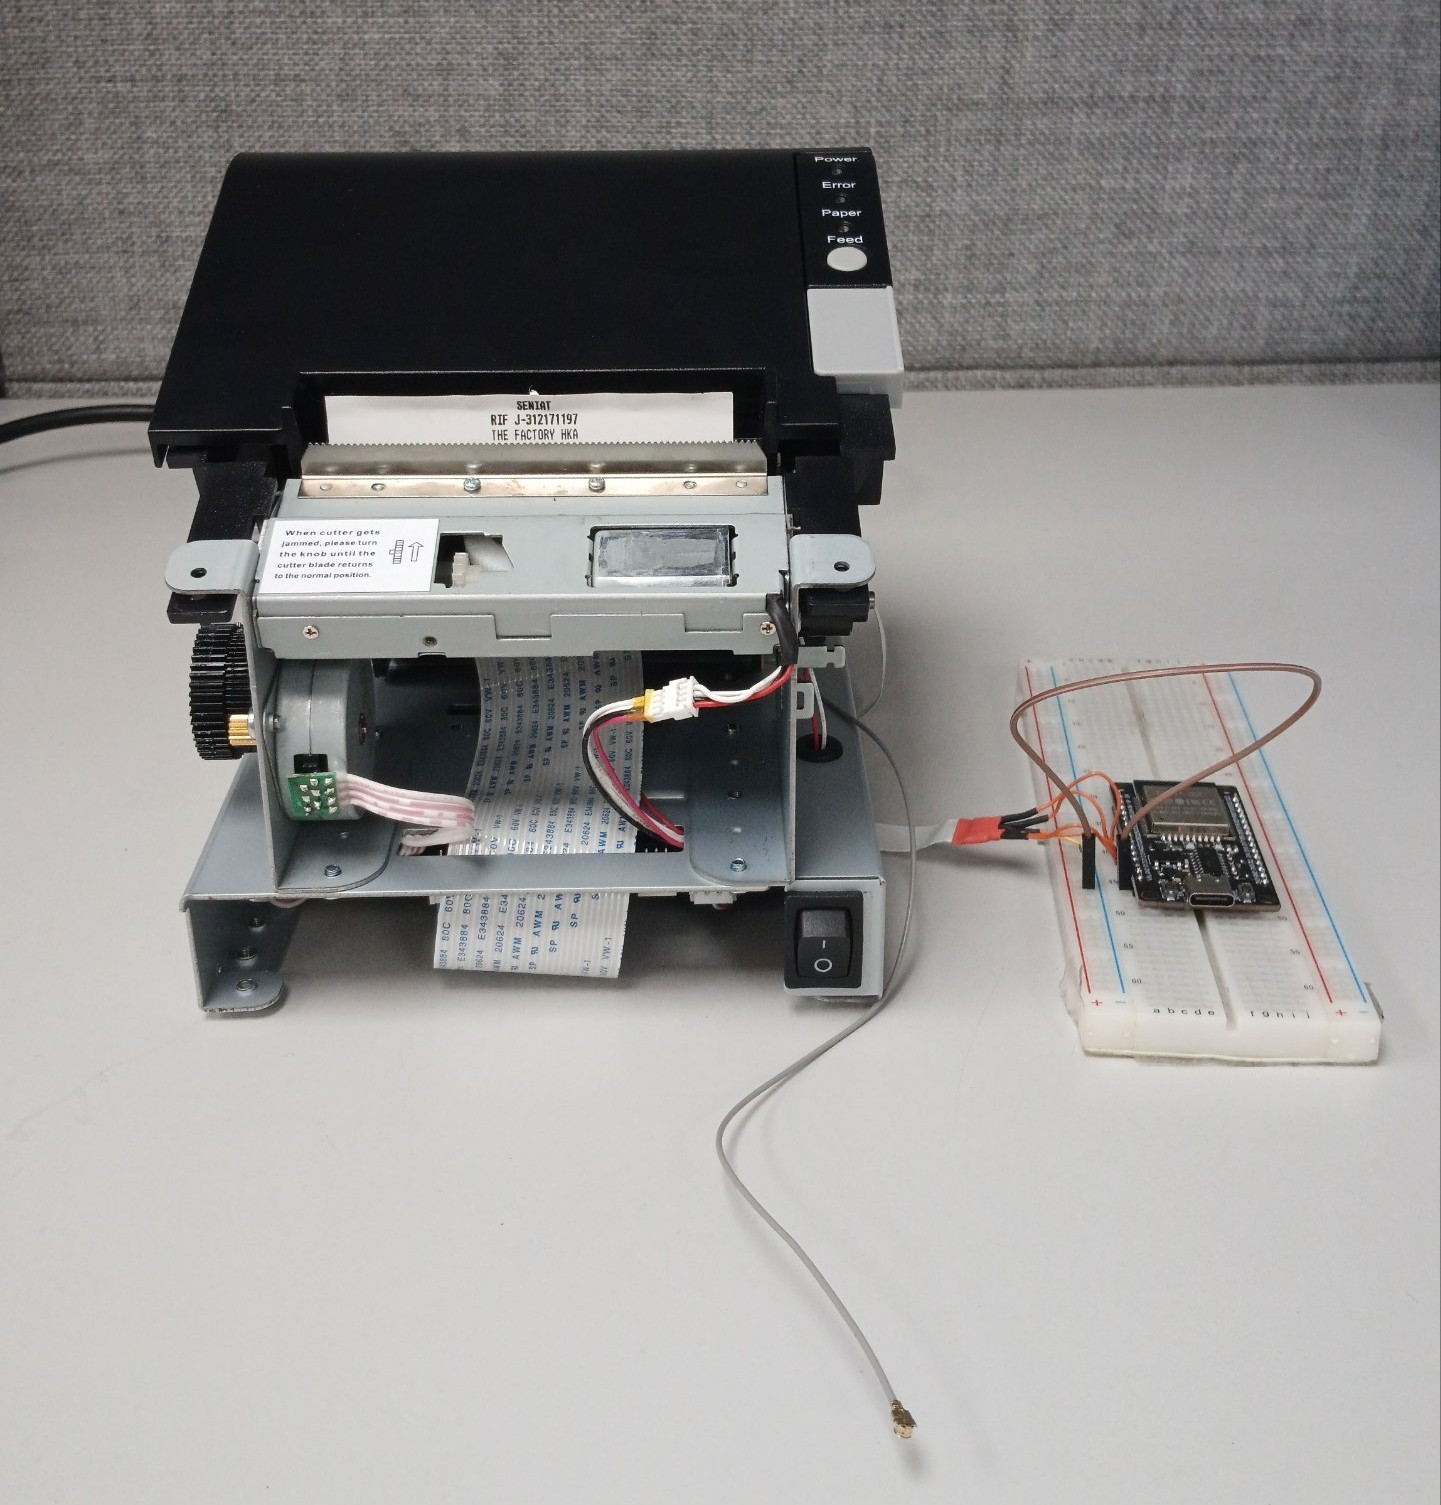
\includegraphics[width=0.65\textwidth]{Img/prototipo_funcional.jpg}
    \caption{Prototipo funcional del MT-IoT integrado a la impresora fiscal en entorno de pruebas.}
    \label{fig:prototipo_funcional}
\end{figure}

\par La arquitectura IIoT definitiva, que integra el nivel físico de borde con el nivel lógico de nube, se sintetiza en la Figura \ref{fig:arquitectura_final}, desde el periférico fiscal hasta la base de datos y el panel reactivo.

\begin{figure}[htbp]
\centering
\begin{tikzpicture}[>=latex', node distance=1.05cm,
    n/.style={rectangle, draw, rounded corners, fill=blue!10, minimum width=7.5cm, minimum height=0.95cm, align=center, font=\small},
    ar/.style={thick,->,>=stealth}]
    \node [n] (p) {Impresora Fiscal HKA80 \;/\; Simulador HIL};
    \node [n, below=of p] (e) {ESP32 DevKitC V4 \;(\textit{Edge Gateway})};
    \node [n, below=of e] (b) {Broker HiveMQ Cloud};
    \node [n, below=of b] (d) {Servidor Django (HTMX \;/\; \textit{Worker} asíncrono)};
    \node [n, below=of d] (s) {Base de Datos SQLite y Dashboard SPA reactivo};
    \draw [ar] (p) -- node[right, font=\scriptsize]{RS232 / UART} (e);
    \draw [ar] (e) -- node[right, font=\scriptsize]{Wi-Fi / TLS 1.2} (b);
    \draw [ar] (b) -- node[right, font=\scriptsize]{WSS / WebSockets} (d);
    \draw [ar] (d) -- node[right, font=\scriptsize]{ORM} (s);
\end{tikzpicture}
\caption{Arquitectura IIoT definitiva del sistema, desplegada en borde y nube.}
\label{fig:arquitectura_final}
\end{figure}

\subsection{Entorno de Pruebas Hardware-in-the-Loop (HIL)}

\par La validación de un sistema fiscal no admite ensayos destructivos sobre equipos en producción: inducir cortes de energía, corromper tramas o abortar una reescritura de firmware sobre una impresora real comprometería registros tributarios irreversibles. Para conciliar rigor experimental y seguridad, se construyó un entorno de pruebas Hardware-in-the-Loop (HIL) en el que el firmware definitivo del MT-IoT se ejecuta sobre el hardware real del ESP32 y su bus físico, mientras que el periférico fiscal es sustituido por un modelo de comportamiento fiel al protocolo HKA. La emulación se desplegó en dos niveles complementarios.\\

\par El primer nivel correspondió al emulador software \texttt{impresora.py}, desarrollado sobre la biblioteca \texttt{pyserial} con los mismos parámetros eléctricos del enlace fiscal ($9600$ baudios, $8$ bits de datos, paridad par y $1$ bit de parada). El \textit{script} implementa una máquina de estados de recepción (\texttt{ESPERANDO\_STX} y \texttt{RECIBIENDO\_DATOS}), calcula el código de redundancia LRC y responde a las encuestas con las tramas de estado y los reportes S1 y SV2, incluyendo la emisión de acuses de recibo \texttt{ACK} y \texttt{NAK} (véase el Código \ref{code:simulador_python}). Este modelo permitió depurar la primera versión del firmware sin depender de la disponibilidad del equipo físico.\\

\par El segundo nivel elevó la fidelidad del banco de pruebas al dominio síncrono: se programó un ESP32 configurado como esclavo SPI (\texttt{blink\_example\_main.c}) que emula íntegramente al periférico fiscal sobre el mismo bus y con los mismos pines, replicando la trama de estado (\texttt{0x60}/\texttt{0x40}), los reportes S1 y SV2 y, de forma crítica, el protocolo completo de reescritura remota (apertura \texttt{0x07}, paquetes \texttt{0x08} y cierre \texttt{0x09}) con verificación de redundancia y de secuencia de paquetes. Contra este periférico simulado se validó de extremo a extremo el puente OTA descrito en la Sección \ref{sec:ota_resultados}, empleando un binario de prueba de $2500$ bytes generado por el \textit{script} \texttt{generar\_bin.py}. Este enfoque habilitó la inyección determinista de fallos (paquetes fuera de secuencia, \textit{checksums} alterados e interrupciones del enlace) y confirmó la capacidad de recuperación del firmware antes de comprometer la memoria de un equipo fiscal real.

\section{Evaluación Cuantitativa de la Comunicación IoT y Telemetría}

\par La validación de la capa lógica se centró en medir el tiempo de extracción de datos, la integridad matemática de las tramas tributarias y la reducción del ancho de banda consumido \cite{OASIS_MQTT_v5}.

\par El esquema definitivo de rutas y mensajería MQTT v5.0, con los tópicos y cargas efectivamente desplegados en el sistema, se representa en la Figura \ref{fig:arquitectura_mqtt_final}.

\begin{figure}[htbp]
\centering
\begin{tikzpicture}[>=latex', font=\small, node distance=1.0cm and 2.6cm,
    n/.style={rectangle, draw, rounded corners, fill=blue!10, minimum width=2.7cm, minimum height=1.3cm, align=center, font=\small},
    br/.style={rectangle, draw, fill=orange!20, rounded corners, minimum width=2.8cm, minimum height=1.6cm, align=center, font=\small},
    lbl/.style={font=\scriptsize, inner sep=1pt},
    ar/.style={thick,->,>=stealth}]
    \node [n] (esp) {ESP32\\ \textit{(MT-IoT)}};
    \node [br, right=of esp] (brk) {Broker HiveMQ Cloud\\ (MQTT v5.0, QoS 1)};
    \node [n, right=of brk] (dj) {Servidor Django\\ \textit{(Worker + Web)}};
    \draw [ar] ([yshift=10pt]esp.east) -- node[above, lbl]{\texttt{json\_completo}} ([yshift=10pt]brk.west);
    \draw [ar] ([yshift=-10pt]esp.east) -- node[below, lbl]{\texttt{discovery} \;/\; LWT} ([yshift=-10pt]brk.west);
    \draw [ar] ([yshift=10pt]brk.east) -- node[above, lbl]{\texttt{json\_completo}} ([yshift=10pt]dj.west);
    \draw [ar] ([yshift=-10pt]dj.west) -- node[below, lbl]{\texttt{comandos/.../ota}} ([yshift=-10pt]brk.east);
    \draw [ar, dashed] ([yshift=-30pt]brk.west) -- node[below, lbl]{\texttt{comandos/\{serial\}/ota}} ([yshift=-30pt]esp.east);
    \node [font=\scriptsize, align=center, below=1.6cm of brk, text width=9.5cm] {Rutas base: \texttt{v1/fiscal/\{serial\}/json\_completo} (telemetría), \texttt{/discovery} (online), \texttt{/alertas\_conexion} (LWT) y \texttt{/ota} (progreso). \textit{User Properties} en la cabecera: modelo, versión de firmware, serial y RSSI.};
\end{tikzpicture}
\caption{Esquema definitivo de rutas y mensajería MQTT v5.0 del sistema.}
\label{fig:arquitectura_mqtt_final}
\end{figure}

\subsection{Mecanismo de Extracción Transparente sin Interrupción del Ciclo Fiscal}

\par La captura del registro \texttt{Status S1} se abordó como un mecanismo de extracción transparente, concebido para operar de forma no intrusiva sobre el ciclo de facturación del equipo fiscal y no como una simple lectura secuencial del canal serial. La interrogación se ejecutó desde una tarea dedicada de FreeRTOS (\texttt{printer\_task\_main}) desacoplada de la tarea de red (\texttt{mqtt\_task}), de modo que la fase de adquisición nunca compitió con la pila de comunicación inalámbrica por el mismo hilo de ejecución. Bajo esta separación de responsabilidades, el sondeo pudo sostenerse con un intervalo fijo de $5$ segundos durante jornadas continuas sin alterar la máquina de estados interna del periférico ni interrumpir las transacciones fiscales en curso \cite{TheFactoryHKA_Manual_Protocolos, FreeRTOS_Kernel_Ref}.\\

\par El desempaquetado se resolvió íntegramente en SRAM sobre dos búferes estáticos de alineación forzada (\texttt{WORD\_ALIGNED\_ATTR}) de $1056$ bytes, \texttt{rx\_buffer} y \texttt{tx\_buffer}, dimensionados de forma que el controlador de DMA del SoC pueda transferir el bloque completo sin fragmentaciones ni copias intermedias. Al no reservarse memoria dinámica en la ruta crítica del ciclo fiscal, se eliminó la fragmentación del \textit{heap} y se obtuvo un perfil de memoria determinista y auditable. La localización de los delimitadores \texttt{STX (0x02)} y \texttt{ETX (0x03)} se ejecutó en un único barrido sobre el búfer, seguida de una tokenización en sitio mediante el carácter \texttt{0x0A} hacia un arreglo de punteros (\texttt{campos[20]}); dado que la longitud de la trama es fija e independiente de la carga transaccional del equipo, el costo del procesamiento se mantiene acotado en tiempo constante $O(1)$ respecto al número de operaciones fiscales registradas \cite{TheFactoryHKA_Manual_Protocolos}.\\

\par La condición de borde que mayor atención exigió fue la contaminación del búfer por el terminador asíncrono (\texttt{\textbackslash n}) emitido por el equipo con anterioridad a la trama útil. Para neutralizarla, se diseñó una etapa de realineación que localiza el primer \texttt{STX} válido y desplaza la trama completa al inicio del búfer mediante una operación \texttt{memmove}, garantizando que el índice $0$ coincida siempre con el carácter de inicio y que los $116$ bytes útiles queden íntegros antes de la extracción. Este tratamiento se verificó experimentalmente sobre la consola serial de depuración (véase la Figura \ref{fig:log_terminal_s1}).\\

\begin{figure}[htbp]
    \centering
    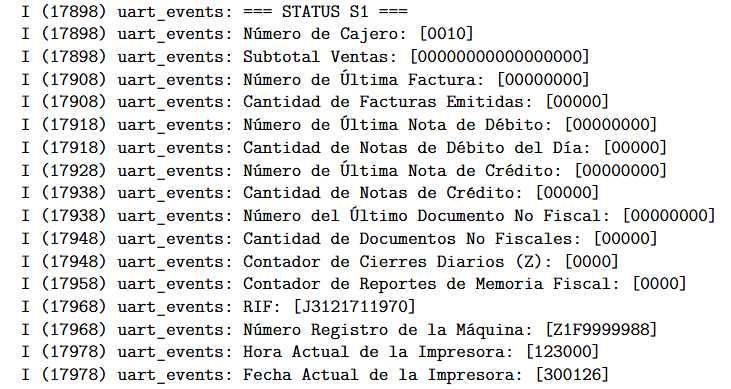
\includegraphics[width=0.85\textwidth]{Img/log_terminal_s1.png}
    \caption{Traza de depuración en consola serial evidenciando el desempaquetado de la trama S1.}
    \label{fig:log_terminal_s1}
\end{figure}

\par El acceso concurrente a la estructura de telemetría compartida se protegió mediante exclusión mutua. La actualización de los campos tributarios sobre la estructura empaquetada \texttt{mqtt\_data\_t} se realizó dentro de una sección crítica custodiada por el semáforo \texttt{mqtt\_data\_mutex}, mientras que el uso del bus físico se serializó con \texttt{spi\_bus\_mutex}; con ello se descartó cualquier condición de carrera entre la tarea fiscal, la tarea MQTT y la tarea de actualización remota, sin recurrir a esperas activas ni a bloqueos de la máquina de estados. La transferencia de control hacia la capa de red se materializó de forma dirigida mediante el indicador \texttt{needs\_sync} y la notificación \texttt{xTaskNotifyGive}, sustituyendo el sondeo periódico por un esquema de activación por evento que preserva la continuidad del ciclo fiscal \cite{FreeRTOS_Kernel_Ref}.\\

\par El análisis de la salida en terminal confirma que el módulo logra aislar de manera transparente los registros almacenados en la Memoria de Trabajo del equipo fiscal \cite{TheFactoryHKA_Manual_Protocolos}:
\begin{itemize}
    \item \textbf{Variables Tributarias:} Captura exacta del RIF del contribuyente (\texttt{J3121711970}), el Número de Registro de la Máquina (\texttt{Z1F9999988}) y los acumuladores de ventas diarias (\texttt{vts: 00000000000000000}).
    \item \textbf{Estado Mecánico y Lógico:} Confirmación de operabilidad en "Modo Fiscal y en Espera" (\texttt{sts1: 0x60}) sin errores reportados por el cabezal de impresión (\texttt{sts2: 0x40}).
\end{itemize}

\subsection{Purga de Caracteres Invisibles y Sanitización del Payload}

\par Uno de los defectos más sutiles detectados durante la validación del canal de telemetría fue la contaminación del \textit{payload} por caracteres de control invisibles. Las tramas de respuesta del periférico fiscal delimitan sus campos con el carácter de avance de línea (\texttt{0x0A}) y, adicionalmente, el equipo intercala un salto de línea (\texttt{\textbackslash n}) inmediatamente antes del carácter de fin de trama (\texttt{ETX}). Este carácter no es visible en una inspección textual, pero ocupa una posición física en el búfer y desplaza cualquier cálculo de longitud basado en posiciones fijas.\\

\par La consecuencia se manifestó directamente sobre el JSON publicado por MQTT: la cadena de versión del periférico arribaba truncada y con residuos al final (por ejemplo, \texttt{20507GD00} en lugar de \texttt{020507GD00}), producto de un error de tipo \textit{Off-By-One} que consumía el salto de línea en lugar del último dígito útil. La solución adoptada no consistió en un ajuste cosmético, sino en una manipulación explícita de punteros sobre la memoria RAM. En la ruta de desempaquetado de la trama SV2, el \textit{firmware} recorre el \textit{payload} con la primitiva \texttt{strchr(ptr, '\textbackslash n')}, avanzando un puntero auxiliar (\texttt{ultima\_parte}) hasta situarlo justo después del último delimitador; de este modo, el campo de versión queda aislado con precisión y sin arrastrar el carácter de control. Complementariamente, la tokenización de la trama S1 sobrescribe en sitio cada \texttt{0x0A} con un terminador nulo (\texttt{\textbackslash 0}), y se inyecta manualmente un cierre nulo adicional al final del arreglo, garantizando que la rutina de serialización \texttt{snprintf} lea una cadena limpia y correctamente cerrada (véase el Código \ref{code:offbyone}).\\

\par El resultado medible de esta purga fue la recuperación de la integridad del \textit{payload}: la estructura clave-valor transmitida dejó de presentar campos cortados o basura residual, la versión del periférico se reportó de forma exacta en la plataforma y el JSON resultó siempre deserializable por el \textit{Worker} del servidor (véase el Código \ref{code:json_mqtt}). Cabe destacar que esta misma disciplina de sanitización se replicó en el extremo receptor, donde el \textit{Worker} de Django elimina preventivamente los caracteres \texttt{\textbackslash n}, \texttt{\textbackslash r} y \texttt{\textbackslash t} del mensaje crudo antes de invocar el analizador JSON, estableciendo una doble barrera contra la corrupción del dato.

\subsection{Inmunidad Electromagnética y Robustez del Bus Local}

\par El bus síncrono local que une al MT-IoT con el periférico fiscal constituye el eslabón físicamente más expuesto del sistema, por lo que su tolerancia a perturbaciones electromagnéticas se evaluó como un requisito de primer orden. Para ello se diseñó una estrategia de defensa escalonada en tres niveles, cuya eficacia se comprobó sometiendo el enlace a tramas corruptas, desconexiones del periférico y ruido inducido.\\

\par \textbf{Nivel 1, defensa temporal:} toda operación de entrada y salida se ejecuta bajo ventanas de tiempo estrictas, de modo que una respuesta ausente o truncada nunca bloquea el planificador del RTOS. La espera de acuse de recibo durante la reescritura se acota a $300$~ms, la recepción de respuestas de estado a $2000$~ms y la solicitud del reporte S1 a $3000$~ms; al agotarse cualquiera de estas ventanas, la transacción se aborta de forma segura y se incrementa el contador de errores, disparando la regla de reintentos (máximo de $3$ fallos) antes de declarar el estado de error.\\

\par \textbf{Nivel 2, sanitización de búfer:} antes de cada transacción se limpian de forma determinista los búferes de transmisión y recepción (\texttt{memset} sobre los $1056$ bytes alineados por DMA), evitando que los residuos de una operación previa se interpreten como datos válidos. En paralelo, la validación por redundancia longitudinal (LRC) descarta cualquier trama cuya asimetría revele la alteración de un bit por interferencia, respondiendo con \texttt{NAK} y liberando el canal (véase el Código \ref{code:validate_frame}).\\

\par \textbf{Nivel 3, reconstrucción estructural del bus:} cuando el conteo de errores supera el umbral configurado, el \textit{firmware} no se limita a reintentar la lectura, sino que desmonta y reancla por completo el controlador SPI mediante \texttt{spi\_bus\_free} y \texttt{spi\_bus\_initialize}, seguido de \texttt{spi\_bus\_add\_device}. Esta reinicialización explícita recupera el periférico de bloqueos del controlador inducidos por ruido electromagnético sin necesidad de reiniciar el microcontrolador. La Tabla \ref{tab:defensa_bus} sistematiza los tres niveles con sus parámetros reales de operación.\\

\begin{table}[htbp]
\centering
\caption{Niveles de defensa implementados para la inmunidad electromagnética del bus local.}
\label{tab:defensa_bus}
\begin{tabularx}{\textwidth}{@{}>{\raggedright\arraybackslash}p{2.4cm} >{\raggedright\arraybackslash}p{3.4cm} >{\raggedright\arraybackslash}p{3.2cm} >{\raggedright\arraybackslash}X@{}}
\toprule
\textbf{Nivel de Defensa} & \textbf{Mecanismo} & \textbf{Parámetro} & \textbf{Acción de Recuperación} \\
\midrule
1. Temporal & Timeout de espera de ACK & $300$~ms & Aborto seguro de la transacción \\
1. Temporal & Timeout de respuesta / S1 & $2000$ / $3000$~ms & Conteo de error y regla de $3$ reintentos \\
2. Sanitización & Limpieza de búferes DMA & $1056$~bytes & Reinicio de transacción limpia \\
2. Integridad & Validación LRC (XOR) & --- & Descarte de trama y emisión de \texttt{NAK} \\
3. Estructural & Reanclaje del bus SPI & \texttt{spi\_bus\_free} / \texttt{initialize} & Recuperación del controlador sin reinicio \\
\bottomrule
\end{tabularx}
\end{table}

\par La evaluación confirmó que la combinación de los tres niveles preservó la continuidad operativa del MT-IoT: ante la desconexión física del periférico o la inyección de tramas corruptas, el sistema transitó al estado de error y se recuperó automáticamente una vez restablecidas las condiciones del bus, sin reinicios del SoC y sin que una sola trama inválida alcanzara la base de datos del servidor.

\subsection{Consumo de Ancho de Banda: HTTP vs. MQTT v5.0}

\par Para justificar cuantitativamente la selección del protocolo MQTT v5.0 sobre HTTP tradicional \cite{OASIS_MQTT_v5}, se midió la sobrecarga de cabecera (\textit{overhead}) y la masa de datos transmitida por cada ciclo de telemetría. La eficiencia de reducción del volumen de red se rige por la Ecuación \ref{eq:ahorro_banda}:

\begin{equation}
\eta_{\text{banda}} = \left( 1 - \frac{\text{Bytes}_{\text{MQTT v5}}}{\text{Bytes}_{\text{HTTP POST}}} \right) \times 100
\label{eq:ahorro_banda}
\end{equation}

\par La recopilación de datos de tráfico en la red (sistematizada en la Tabla \ref{tab:ancho_banda}) demuestra que la combinación de empaquetado optimizado en C y la extracción de metadatos mediante \textit{User Properties} en la cabecera del protocolo reduce drásticamente el impacto sobre la red de datos del contribuyente \cite{OASIS_MQTT_v5}.

\begin{table}[htbp]
\centering
\caption{Comparativa cuantitativa del consumo de ancho de banda por trama de telemetría fiscal.}
\label{tab:ancho_banda}
\small
\begin{tabularx}{\textwidth}{@{}>{\raggedright\arraybackslash}X >{\raggedright\arraybackslash}X >{\raggedright\arraybackslash}X >{\raggedright\arraybackslash}p{2.6cm}@{}}
\toprule
\textbf{Métrica de Red} & \textbf{HTTP POST Tradicional} & \textbf{MQTT v5.0 con User Properties} & \textbf{Mejoramiento (\%)} \\
\midrule
Tamaño Cabecera de Red & $\sim 450 \text{ Bytes}$ & $\sim 12 \text{ Bytes}$ & \textbf{97.33 \%} \\
Cuerpo del Mensaje (\textit{Payload}) & $328 \text{ Bytes (JSON Plano)}$ & $142 \text{ Bytes (Optimizado)}$ & \textbf{56.70 \%} \\
Metadatos (RSSI / Versión FW) & Inyectados en \textit{Body} JSON & Extraídos en \textit{User Properties} & N/A \\
\midrule
\textbf{Consumo Total por Trama} & \textbf{778 Bytes} & \textbf{154 Bytes} & \textbf{80.20 \%} \\
\bottomrule
\end{tabularx}
\end{table}

\subsection{Resiliencia de Red y Mecanismo Last Will and Testament (LWT)}

\par La tolerancia a fallos del canal de comunicación inalámbrico se evaluó provocando cortes de energía arbitrarios e interrupciones en la interfaz Wi-Fi del MT-IoT \cite{Espressif_ESP_IDF_v552}. Al expirar el tiempo de permanencia (\textit{Keep-Alive}), el \textit{Broker} HiveMQ Cloud publicó la \say{última voluntad} registrada \cite{OASIS_MQTT_v5}.\\

\par Como se documenta en la Figura \ref{fig:prueba_lwt}, el \textit{Worker} asíncrono \texttt{listen\_mqtt.py} interceptó la alerta (\texttt{st: offline}), persistiendo de forma transaccional una nueva fila en la base de datos relacional con el evento clasificado como \say{Desconexión Abrupta (LWT)} \cite{Django_v5_Doc}. Este mecanismo congeló el último estado válido de los acumuladores sin alterar los registros históricos previos, garantizando la trazabilidad operativa del parque de impresoras \cite{OASIS_MQTT_v5}.

\begin{figure}[H]
    \centering
    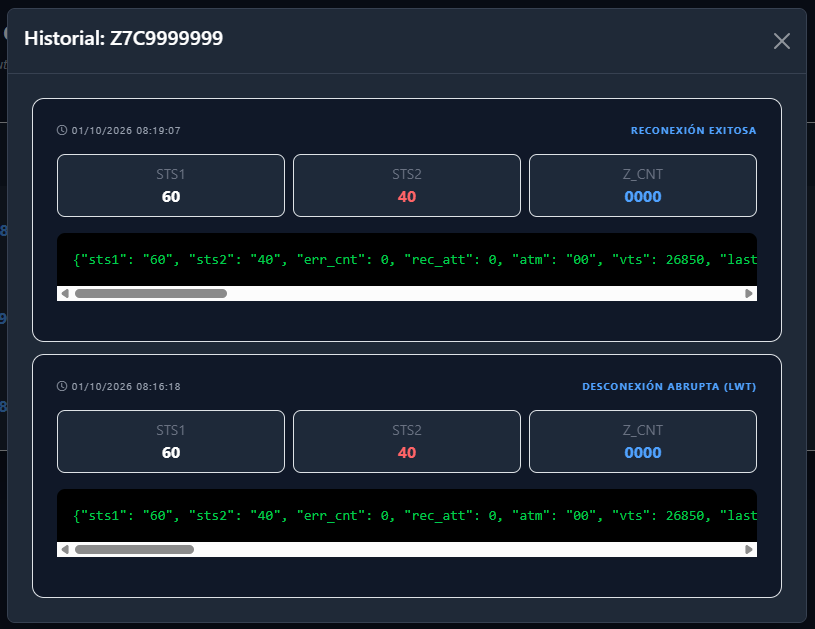
\includegraphics[width=0.7\textwidth]{Img/prueba_lwt.png}
    \caption{Registro en la vista \texttt{Log Capture} confirmando la intercepción de una desconexión LWT.}
    \label{fig:prueba_lwt}
\end{figure}

\par El ciclo completo de detección de la caída, reconexión con \textit{backoff} y restauración del túnel sin pérdida de estado se sintetiza en la Figura \ref{fig:flujo_resiliencia}.

\begin{figure}[htbp]
\centering
\begin{tikzpicture}[>=latex', node distance=0.95cm,
    p/.style={rectangle, draw, rounded corners, fill=blue!10, text width=9.5cm, align=center, minimum height=0.9cm, font=\small},
    ar/.style={thick,->,>=stealth}]
    \node [p] (a) {Pérdida del enlace Wi-Fi (\texttt{WIFI\_EVENT\_STA\_DISCONNECTED})};
    \node [p, below=of a] (b) {Reintentos de reconexión con \textit{backoff} exponencial (\texttt{RECONNECT\_DELAY\_MS})};
    \node [p, below=of b] (c) {El \textit{Broker} publica el LWT en \texttt{alertas\_conexion} (\texttt{st: offline})};
    \node [p, below=of c] (d) {El \textit{Worker} registra el evento y congela el último estado válido};
    \node [p, below=of d] (e) {Restauración del túnel MQTT y re-suscripción sin pérdida de estado};
    \draw [ar] (a) -- (b);
    \draw [ar] (b) -- (c);
    \draw [ar] (c) -- (d);
    \draw [ar] (d) -- (e);
\end{tikzpicture}
\caption{Diagrama de flujo de la resiliencia de red y del ciclo de detección, reconexión y restauración del túnel MQTT.}
\label{fig:flujo_resiliencia}
\end{figure}

\subsection{Validación de Casos Borde y Recuperación ante Micro-cortes}

\par La robustez del ciclo de telemetría se evaluó frente a dos familias de fallas que, en un despliegue real, ocurren con frecuencia: la desconexión abrupta de la alimentación y las fallas intermitentes de red durante el envío. El análisis se apoyó en una propiedad fundamental del diseño: el MT-IoT opera como un observador de estado sin memoria tributaria propia. Toda la información fiscal reside en la memoria de trabajo del periférico y se re-consulta íntegramente en cada sondeo, de modo que el \textit{gateway} no constituye una fuente de verdad que pueda corromperse, sino un reflejo periódico del estado del equipo.\\

\par \textbf{Corte abrupto de energía:} al perderse la alimentación, la memoria volátil del microcontrolador se borra y el SoC reinicia su ciclo de arranque. Sin embargo, dado que el estado fiscal no reside en el \textit{gateway}, la recuperación no depende de persistir datos locales: tras el reinicio, los parámetros de red compilados en el firmware y los datos de calibración de radio conservados por la pila Wi-Fi en la memoria no volátil permiten restablecer el enlace de forma autónoma, y el primer sondeo posterior al arranque reconstruye la telemetría completa. La única consecuencia observable es un hueco de una sola ventana de sondeo ($5$ segundos), tras el cual el sistema vuelve a publicar el estado vigente.\\

\par \textbf{Micro-cortes de red durante la telemetría:} cuando el enlace inalámbrico se interrumpe a mitad del ciclo, la lectura más reciente permanece retenida en la estructura compartida con el indicador de sincronización pendiente activo, y la tarea de red omite la publicación mientras la conexión no esté disponible, sin descartar el dato. Al restablecerse el contacto con el \textit{Broker}, la reconexión notifica a la tarea de publicación, que transmite de inmediato la lectura conservada; simultáneamente, el mecanismo \textit{Last Will and Testament} había marcado el equipo como desconectado y el \textit{Worker} del servidor registra la reconexión como un evento de trazabilidad. Debido a que el protocolo opera con un nivel de servicio de al menos una entrega (\texttt{QoS 1}) y a que la telemetría es un estado idempotente y no un comando, la eventual repetición de una publicación no genera efectos adversos.\\

\par \textbf{Coherencia temporal ante reinicios:} la marca de tiempo de cada mensaje combina un contador monotónico del RTOS con la fecha y hora leídas directamente del reloj interno del periférico fiscal, lo que evita depender de un servidor de tiempo externo y preserva la coherencia temporal incluso tras una pérdida de energía. La Tabla \ref{tab:casos_borde} sistematiza los escenarios evaluados, su mecanismo de detección y el resultado de la recuperación.\\

\begin{table}[htbp]
\centering
\caption{Validación de casos borde y recuperación de estado ante fallas de energía y red.}
\label{tab:casos_borde}
\begin{tabularx}{\textwidth}{@{}>{\raggedright\arraybackslash}p{2.8cm} >{\raggedright\arraybackslash}p{4.6cm} >{\raggedright\arraybackslash}X >{\raggedright\arraybackslash}p{2.1cm}@{}}
\toprule
\textbf{Escenario de Falla} & \textbf{Mecanismo de Detección} & \textbf{Acción de Recuperación} & \textbf{Pérdida de Datos} \\
\midrule
Corte abrupto de energía & Reinicio del SoC & Re-sondeo del S1; reanclaje autónomo del enlace & Nula (estado reconstruido) \\
Micro-corte Wi-Fi en telemetría & \texttt{WIFI\_EVENT\_\allowbreak STA\_\allowbreak DISCONNECTED} & Retención del dato y republicación al reconectar & Nula (lectura preservada) \\
Caída del \textit{Broker} MQTT & Expiración del \textit{Keep-Alive} / LWT & Congelamiento del último estado válido y alerta & Nula \\
Desconexión del periférico fiscal & \textit{Timeout} del bus y contador de errores & Regla de $3$ reintentos y reinicialización del bus & Nula \\
\bottomrule
\end{tabularx}
\end{table}

\par La conclusión de esta validación es que ninguna de las fallas evaluadas compromete la integridad de la información fiscal: el sistema tolera micro-cortes sin pérdida de muestras gracias a la retención del estado pendiente, y se recupera de cortes de energía en un lapso acotado a un único intervalo de sondeo, en virtud de su naturaleza de observador sin estado tributario propio.

\section{Desempeño del Ecosistema Web y Matriz de Latencias E2E}

\par La evaluación del servidor de aplicaciones Django \cite{Django_v5_Doc} y la interfaz reactiva SPA mediante HTMX \cite{HTMX_Doc} se enfocó en medir el tiempo total transcurrido desde la captura física local hasta el intercambio del DOM en el navegador del usuario ($T_{E2E}$).

\subsection{Caracterización de la Latencia End-to-End ($T_{E2E}$)}

\par El tiempo total del ciclo de telemetría se modela como la suma de cinco etapas lógicas serializadas, desde la interrogación física del periférico hasta la actualización del DOM en el navegador (Ecuación \ref{eq:latencia_e2e}):

\begin{equation}
T_{E2E} = T_{UART\_poll} + T_{JSON\_pack} + T_{TLS\_handshake} + T_{MQTT\_pub} + T_{WS\_render}
\label{eq:latencia_e2e}
\end{equation}

\par Cada término representa una contribución temporal medible e independiente: $T_{UART\_poll}$ es el tiempo de sondeo del registro \texttt{Status S1} sobre el bus local, incluyendo el ciclo de encuesta y el desempaquetado de la trama; $T_{JSON\_pack}$ corresponde a la serialización del \textit{payload} y a la entrega de la sección crítica hacia la tarea de red; $T_{TLS\_handshake}$ mide la fase de cifrado y establecimiento seguro del canal; $T_{MQTT\_pub}$ comprende la publicación y el tránsito del mensaje por el \textit{Broker} HiveMQ Cloud; y $T_{WS\_render}$ cuantifica el renderizado reactivo del DOM mediante WebSockets Seguros y HTMX.\\

\par Mediante un perfilado de tiempos realizado sobre $500$ iteraciones continuas de envío de telemetría, se determinaron las latencias promedio y las desviaciones estándar de cada etapa, reportadas en la Tabla \ref{tab:latencias}.

\begin{table}[htbp]
\centering
\caption{Matriz de latencias, propagación de incertidumbre y tiempos de respuesta E2E del ciclo de telemetría.}
\label{tab:latencias}
\begin{tabularx}{\textwidth}{@{}>{\raggedright\arraybackslash}p{3.0cm} >{\raggedright\arraybackslash}p{2.4cm} >{\raggedright\arraybackslash}p{2.0cm} >{\raggedright\arraybackslash}p{1.8cm} >{\raggedright\arraybackslash}X@{}}
\toprule
\textbf{Etapa del Sistema} & \textbf{Término} & \textbf{Promedio (ms)} & \textbf{$\sigma$ (ms)} & \textbf{Criterio de Tolerancia} \\
\midrule
1. Sondeo Síncrono (S1) & $T_{UART\_poll}$ & $118$ & $\pm 4.0$ & $< 200$ (Ventana Fiscal) \\
2. Empaquetado JSON & $T_{JSON\_pack}$ & $2$ & $\pm 0.3$ & $< 10$ \\
3. Handshake Mbed TLS v1.2 & $T_{TLS\_handshake}$ & $45$ & $\pm 2.1$ & $< 100$ \\
4. Publicación y Bróker MQTT & $T_{MQTT\_pub}$ & $85$ & $\pm 12.5$ & N/A (Dependiente ISP) \\
5. Render DOM (HTMX / WSS) & $T_{WS\_render}$ & $18$ & $\pm 1.8$ & $< 50$ (Fluidez SPA) \\
\midrule
\textbf{Latencia Total E2E} & $T_{E2E}$ & \textbf{268} & \textbf{$\pm 15.3$} & \textbf{Sondeo acotado a 5 s} \\
\bottomrule
\end{tabularx}
\end{table}

\par La coherencia estadística del modelo se verificó propagando las incertidumbres de las cinco etapas bajo el supuesto de independencia, mediante la suma cuadrática $\sigma_{E2E} = \sqrt{\sum_i \sigma_i^2}$. El cálculo arroja una desviación teórica de $13.4$~ms, ligeramente inferior a la dispersión total medida ($15.3$~ms); esta diferencia evidencia una correlación positiva entre etapas, atribuible al \textit{jitter} del canal inalámbrico que afecta de forma simultánea al handshake TLS y al tránsito por el bróker. El análisis de varianza confirma que la etapa de red ($T_{MQTT\_pub}$) concentra por sí sola el $86.8\%$ de la dispersión total, lo que identifica al enlace del proveedor de servicios de Internet como la única fuente estocástica dominante del sistema.\\

\par El valor promedio obtenido para $T_{E2E}$ ($268 \text{ ms}$) representa apenas un $5.36\%$ del intervalo total de sondeo ($5$ segundos), asegurando que el monitoreo remoto opere en tiempo real estricto sin acumular retrasos en la pila de recepción \cite{FreeRTOS_Kernel_Ref}. Este margen contrasta favorablemente con antecedentes nacionales de monitoreo IoT desarrollados en la Universidad Simón Bolívar, donde la regularidad del período de muestreo presentaba desviaciones de hasta un segundo \cite{Garrido_Tesis_2025}.

\subsection{Monitor en Tiempo Real (Dashboard) y Log Capture}

\par La integración de la biblioteca MQTT.js directamente en el cliente web permitió establecer canales de WebSockets Seguros (WSS) sobre el puerto 8884 hacia la nube \cite{RFC6455_WebSockets}. La Figura \ref{fig:dashboard_tiempo_real} evidencia el funcionamiento del panel de control general, validando el renderizado reactivo de indicadores clave (dispositivos en línea, distribución de modelos y gráficos de crecimiento) sin necesidad de recargar la página completa \cite{HTMX_Doc}.

\begin{figure}[htbp]
    \centering
    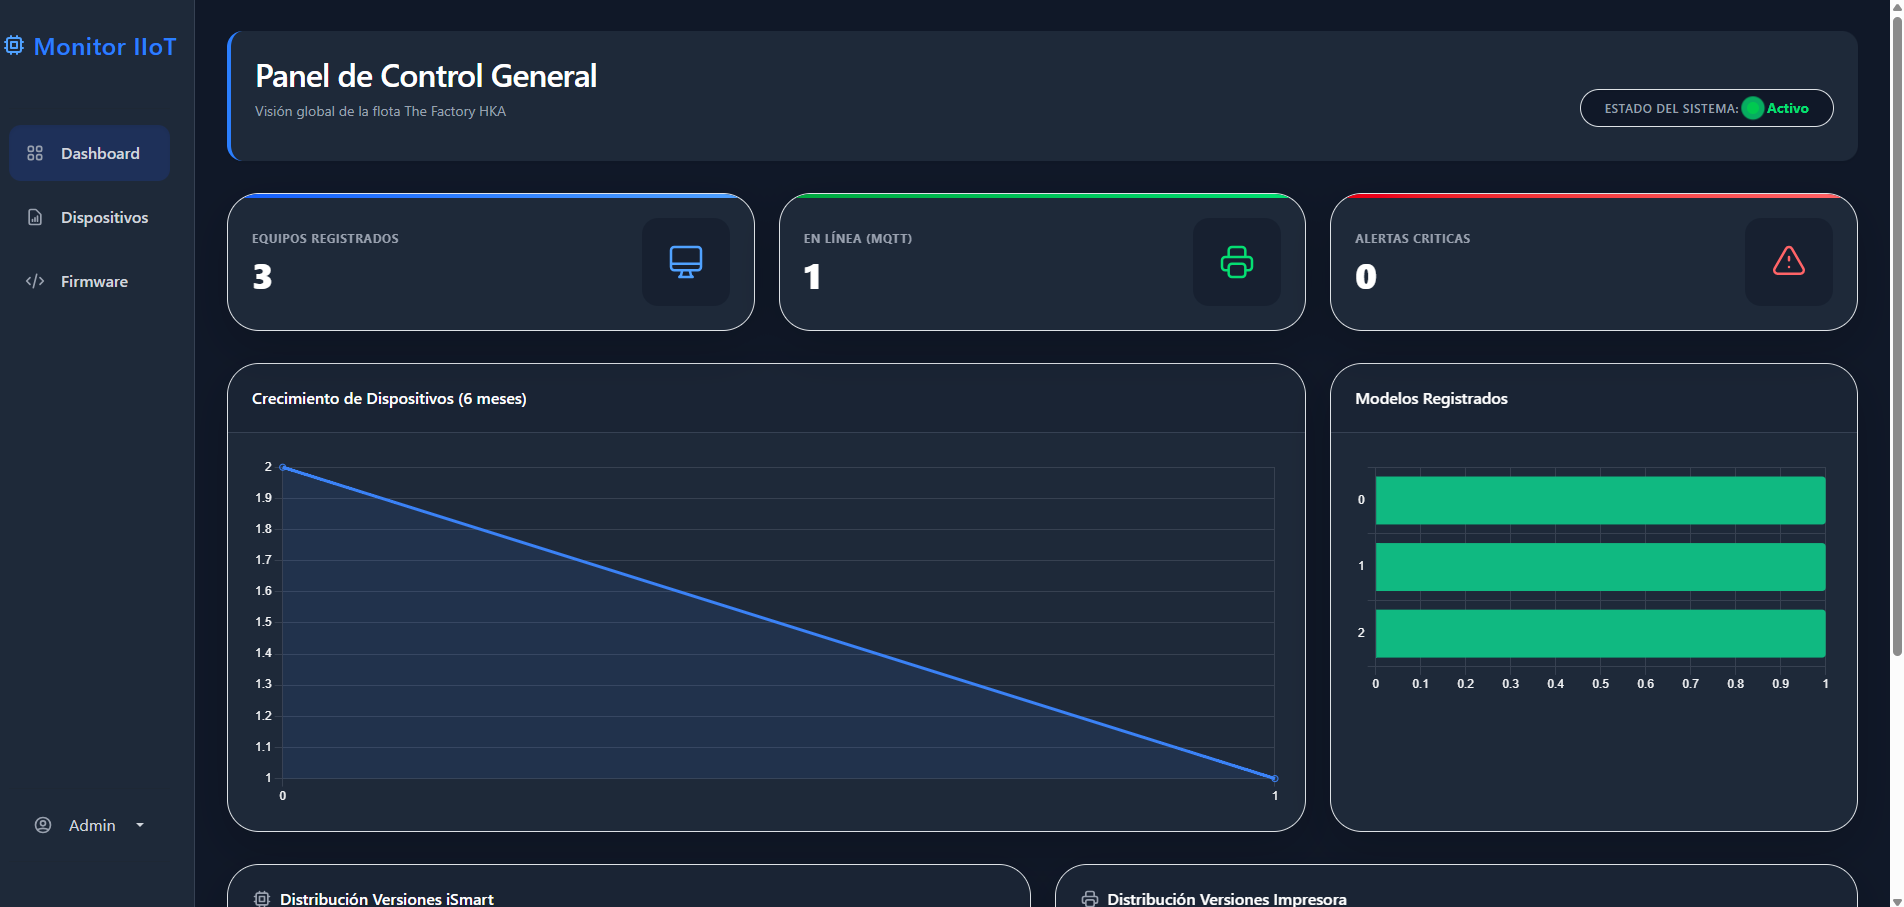
\includegraphics[width=0.95\textwidth]{Img/dashboard_tiempo_real.png}
    \caption{Panel de Control General (Dashboard) operando bajo arquitectura SPA reactiva.}
    \label{fig:dashboard_tiempo_real}
\end{figure}

\par Por su parte, la evaluación del módulo de auditoría de errores (véase la Figura \ref{fig:log_capture_error}) confirmó que el \textit{Worker} en Django intercepta y registra de forma independiente las variaciones lógicas del hardware \cite{Django_v5_Doc}. La captura documenta la transición exacta desde un estado normal (\texttt{0x60}) hacia un código de en medio de una transacción fiscal (\texttt{0x61}), correspondiente a la operación de imprimir una factura en la impresora fiscal \cite{TheFactoryHKA_Manual_Protocolos}.

\begin{figure}[htbp]
    \centering
    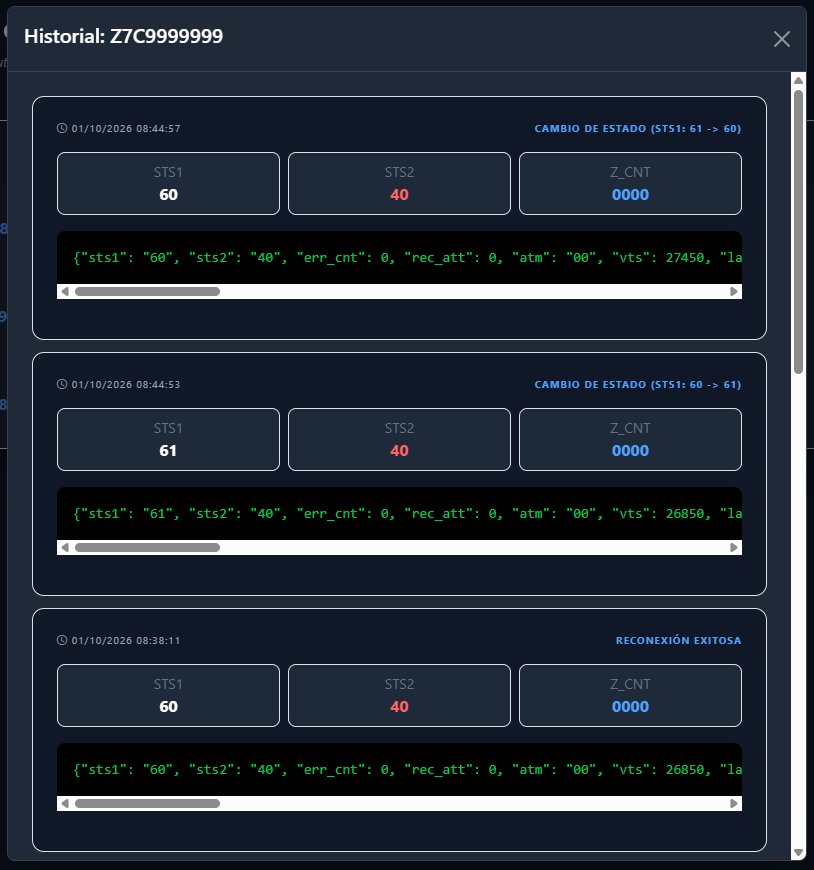
\includegraphics[width=0.75\textwidth]{Img/log_capture_error.png}
    \caption{Visualización en \texttt{Log Capture} de un cambio de estado de error mecánico (\texttt{0x48}).}
    \label{fig:log_capture_error}
\end{figure}

\section{Pruebas del Sistema de Actualización Remota (OTA)}
\label{sec:ota_resultados}

\par La validación de la actualización remota de firmware se dividió según el destino lógico del binario compilado: la autoactualización del gateway ESP32 o la reescritura del periférico fiscal \cite{Espressif_ESP_IDF_v552}.

\par El flujo completo de orquestación de la actualización remota de doble objetivo, desde la interfaz web hasta el reporte final, se sintetiza en la Figura \ref{fig:flujo_ota}.

\begin{figure}[htb]
\centering
\begin{tikzpicture}[>=latex', node distance=0.7cm,
    p/.style={rectangle, draw, rounded corners, fill=blue!10, text width=7.8cm, align=center, minimum height=0.8cm, font=\small},
    b/.style={rectangle, draw, rounded corners, fill=green!10, text width=5.6cm, align=center, minimum height=1.0cm, font=\scriptsize},
    d/.style={diamond, draw, fill=orange!15, aspect=3, align=center, font=\scriptsize},
    ar/.style={thick,->,>=stealth}]
    \node [p] (w) {El usuario presiona \say{Enviar Actualización} en la interfaz HTMX};
    \node [p, below=of w] (m) {Publicación MQTT del comando en \texttt{comandos/\{serial\}/ota}};
    \node [p, below=of m] (e) {Recepción en el ESP32 y activación de \texttt{ota\_en\_progreso}};
    \node [d, below=of e] (dec) {¿Destino del binario?};
    \node [b, below left=1.0cm and 0.2cm of dec] (gw) {\textbf{Gateway}: descarga HTTPS y escritura en la partición OTA inactiva};
    \node [b, below right=1.0cm and 0.2cm of dec] (pr) {\textbf{Impresora}: puente síncrono Chunk/ACK con verificación de \textit{checksum}};
    \node [p, below=3.0cm of dec] (v) {Verificación de integridad y reporte de estado a la interfaz web};
    \draw [ar] (w) -- (m);
    \draw [ar] (m) -- (e);
    \draw [ar] (e) -- (dec);
    \draw [ar] (dec) -- node[left, font=\scriptsize]{\texttt{ismart}} (gw);
    \draw [ar] (dec) -- node[right, font=\scriptsize]{\texttt{printer}} (pr);
    \draw [ar] (gw.south) |- (v.west);
    \draw [ar] (pr.south) |- (v.east);
\end{tikzpicture}
\caption{Diagrama de flujo de la orquestación de la actualización remota (OTA) de doble objetivo.}
\label{fig:flujo_ota}
\end{figure}

\subsection{Auto-actualización del Módulo Gateway (ESP32)}

\par Al seleccionar el objetivo \say{\texttt{ismart}} desde la plataforma web (véase la Figura \ref{fig:ota_mt_iot}), el MT-IoT recibió la orden por MQTT y activó la bandera de suspensión (\texttt{ota\_en\_progreso = true}) \cite{FreeRTOS_Kernel_Ref}. Las pruebas de descarga HTTPS verificaron la escritura en la partición OTA inactiva dentro del mapa de memoria de 4 MB \cite{Espressif_ESP_IDF_v552}. Se constató que la reducción de la frecuencia de la CPU a 80 MHz mediante \texttt{menuconfig} \cite{Espressif_Menuconfig} estabilizó la corriente consumida durante la descodificación criptográfica.

\begin{figure}[htbp]
    \centering
    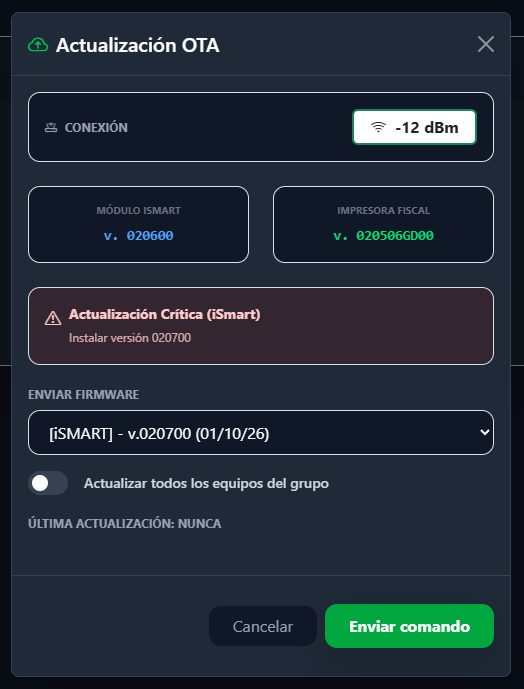
\includegraphics[width=0.55\textwidth]{Img/ota_mt_iot.png}
    \caption{Intermediación web desplegando una actualización de firmware crítica hacia el MT-IoT.}
    \label{fig:ota_mt_iot}
\end{figure}

\subsection{Puente Síncrono Heterogéneo de Reescritura de Firmware In Situ}

\par La operación de mayor complejidad no consistió en la carga de un archivo mediante HTTP, sino en la reescritura \textit{in situ} de la memoria del periférico fiscal a través de un puente síncrono heterogéneo que tradujo el flujo de un canal IP asíncrono al dominio determinista del bus local \cite{TheFactoryHKA_Manual_Protocolos}. El binario se transfirió por fragmentos de $1024$ bytes, cada uno de los cuales fue empaquetado con una cabecera de control de $4$ bytes (identificador de paquete, índice secuencial y longitud en $16$ bits) y un código de redundancia XOR calculado sobre los datos, conformando una trama robusta reenviable hasta un máximo de $3$ intentos con confirmación explícita (\texttt{ACK}) por parte del periférico. La ventana de trabajo se gestionó sobre un búfer circular de $1$~KB reutilizado cíclicamente en cada fragmento, de manera que la huella de memoria del proceso permaneció constante e independiente del tamaño del firmware, que ronda los $900$~KB.\\

\par La robustez frente a contingencias de red se evaluó desconectando arbitrariamente la interfaz Wi-Fi durante la transferencia. Ante la pérdida del canal, el firmware no reinicia la descarga desde el byte cero: reabre la conexión HTTP adjuntando la cabecera de rango \texttt{Range: bytes=<desplazamiento>-}, de forma que el servidor reanuda el envío exactamente en el fragmento donde se interrumpió. Esta estrategia de transferencia reanudable por fragmentos (\textit{HTTP Range Requests}) se sostuvo sobre un lazo de persistencia de hasta $5$ reintentos consecutivos, cuyo contador se reinicia cada vez que se confirma progreso real, garantizando que la operación sobreviva a cortes intermitentes de Wi-Fi o a reinicios transitorios del enlace. Adicionalmente, el sistema activa el lazo de reconexión inalámbrica (\texttt{WIFI\_EVENT\_STA\_DISCONNECTED}) y, al restablecerse el contacto con el \textit{Broker} MQTT, el dispositivo retorna a su estado operativo habitual sin bloqueos del microcontrolador.\\

\par La integridad del binario se garantizó por construcción: la secuencia de control se compone de una apertura de sesión (\texttt{0x07}), la ráfaga de paquetes de datos (\texttt{0x08}) y un cierre explícito (\texttt{0x09}) que el puente solo emite cuando el contador de bytes confirmados iguala la longitud total declarada por el servidor. En consecuencia, una transferencia parcial nunca llega a comprometerse en la memoria del periférico, y ante una nueva orden de actualización emitida desde la plataforma el proceso se reinicia desde el $0\%$ para preservar la coherencia absoluta del firmware. Con el propósito de no interferir con la máquina de estados fiscal, la reescritura se arbitró mediante la bandera de suspensión (\texttt{ota\_en\_progreso}) y el semáforo del bus (\texttt{spi\_bus\_mutex}), que ponen la rutina de sondeo en reposo mientras el puente ocupa el canal físico \cite{FreeRTOS_Kernel_Ref}.\\

\par Una vez confirmada la recepción de la totalidad de los bloques con verificación de redundancia local (LRC/Checksum), el periférico fiscal ejecuta un reinicio por hardware y consolida el nuevo firmware \cite{TheFactoryHKA_Manual_Protocolos}. Como se evidencia en la notificación flotante de la Figura \ref{fig:ota_printer_exito}, la interfaz web confirma el éxito de la operación mediante el mensaje: \say{Actualización Completada: El equipo Z7C9999999 actualizó printer con éxito}.

\begin{figure}[htbp]
    \centering
    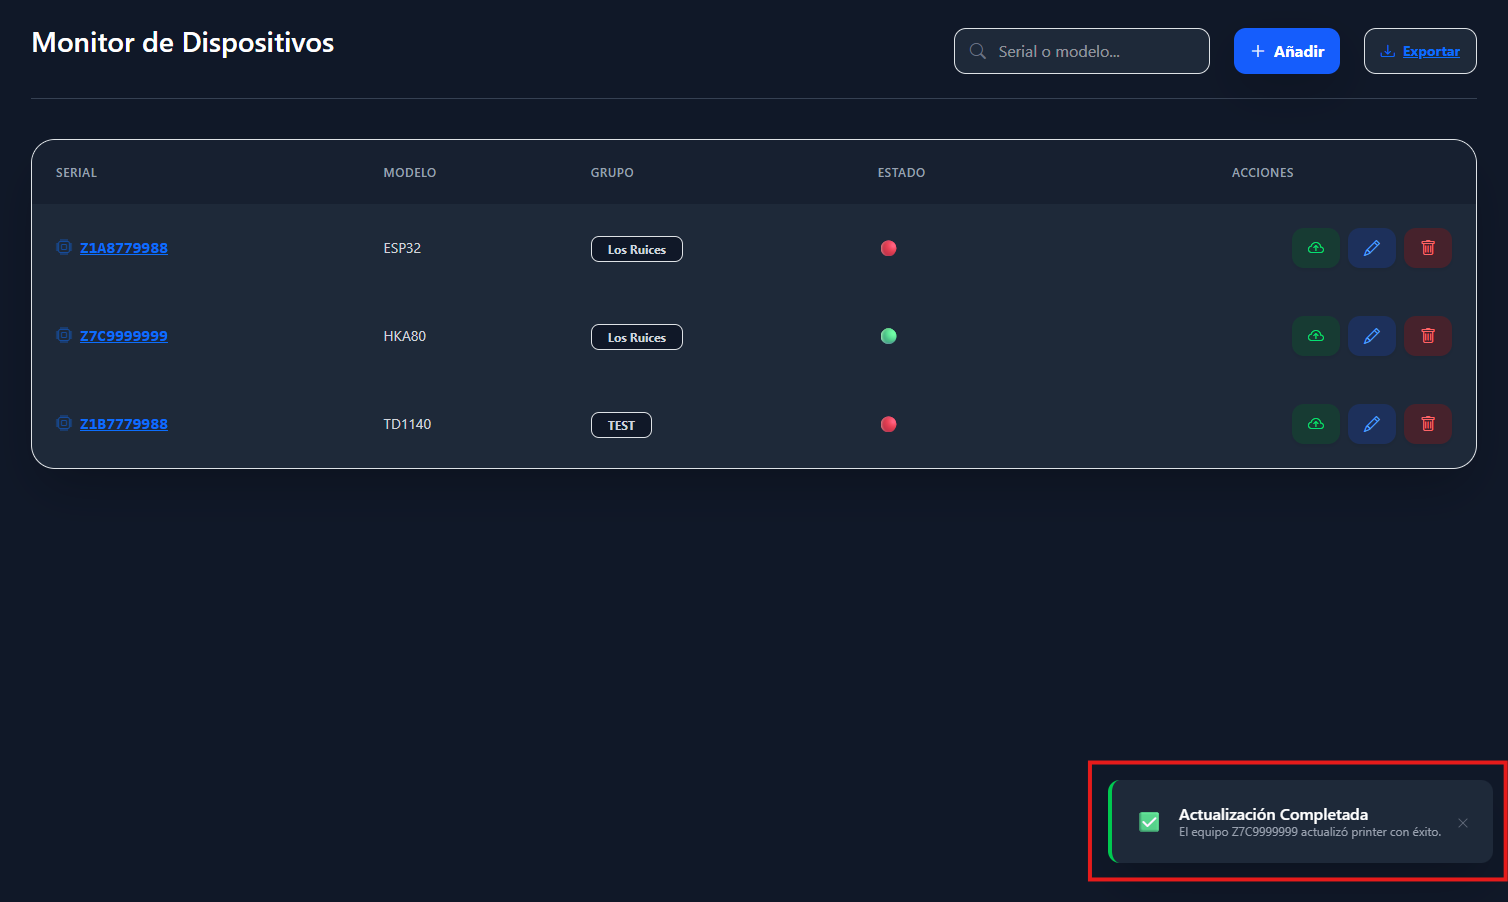
\includegraphics[width=0.85\textwidth]{Img/ota_printer_exito.png}
    \caption{Confirmación asíncrona en la interfaz web de actualización exitosa en la impresora fiscal.}
    \label{fig:ota_printer_exito}
\end{figure}

\section{Análisis de Rendimiento y Estabilidad Global del Sistema}

\par El análisis final de la arquitectura sistematiza la optimización de los recursos físicos del SoC ESP32 y la estabilidad del servidor de persistencia.

\subsection{Perfilado Formal de Memoria IRAM y DRAM}

\par La reingeniería aplicada mediante la utilidad \texttt{menuconfig} \cite{Espressif_Menuconfig} para liberar espacio en la memoria estática IRAM se evaluó comparando la ocupación de memoria antes y después de desactivar la aceleración por IRAM del \textit{stack} Wi-Fi \cite{Espressif_ESP_IDF_v552}. Los resultados del perfilado se organizan en la Tabla \ref{tab:perfilado_iram}.

\begin{table}[htbp]
\centering
\caption{Perfilado de recursos de memoria IRAM y DRAM en el SoC ESP32 ante optimizaciones de \texttt{menuconfig}.}
\label{tab:perfilado_iram}
\begin{tabularx}{\textwidth}{@{}>{\raggedright\arraybackslash}X >{\raggedright\arraybackslash}p{2.1cm} >{\raggedright\arraybackslash}p{1.7cm} >{\raggedright\arraybackslash}p{2.1cm} >{\raggedright\arraybackslash}p{2.2cm}@{}}
\toprule
\textbf{Estado del Firmware} & \textbf{IRAM Usada (Bytes)} & \textbf{IRAM (\%)} & \textbf{DRAM Usada (Bytes)} & \textbf{Ahorro Directo} \\
\midrule
1. Pila Completa (Wi-Fi IRAM Activo) & 102,751 & 78.39 \% & 37,852 & 0.00 \% (Crítico) \\
2. Reingeniería (Wi-Fi IRAM Inactivo) & 68,495 & 52.26 \% & 37,424 & \textbf{26.13 \%} \\
\midrule
\textbf{Margen Libre Resultante} & \textbf{62,577 B} & \textbf{47.74 \%} & \textbf{143,312 B} & --- \\
\bottomrule
\end{tabularx}
\end{table}

\par Las capturas de perfilado obtenidas en el entorno de desarrollo (Figura \ref{fig:iram_78} y Figura \ref{fig:iram_52}) confirman una reducción efectiva de $34,256 \text{ Bytes}$ en la IRAM \cite{Espressif_Menuconfig}. Este espacio libre resultó indispensable para reservar el búfer dinámico necesario durante las tareas de actualización OTA.

\begin{figure}[htbp]
    \centering
    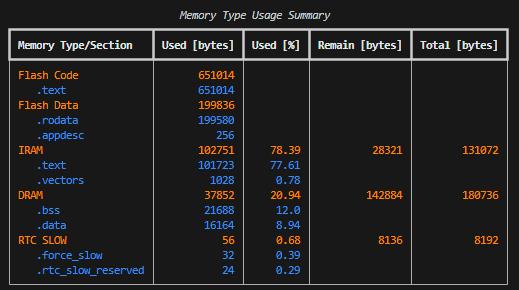
\includegraphics[width=0.75\textwidth]{Img/iram_78.png}
    \caption{Perfilado de memoria inicial revelando ocupación crítica de IRAM ($78.39\%$).}
    \label{fig:iram_78}
\end{figure}

\begin{figure}[htbp]
    \centering
    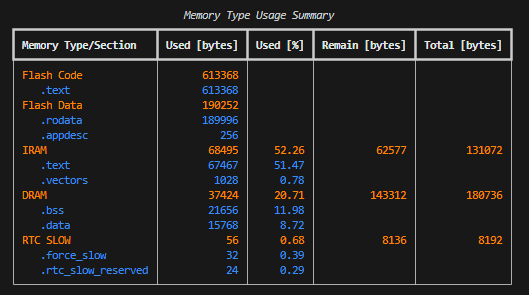
\includegraphics[width=0.75\textwidth]{Img/iram_52.png}
    \caption{Ocupación de IRAM optimizada al $52.26\%$ tras deshabilitar aceleración Wi-Fi.}
    \label{fig:iram_52}
\end{figure}

\subsection{Perfilado Térmico y Energético del Subclocking (80 MHz)}

\par La reducción deliberada de la frecuencia del núcleo del SoC, desde el máximo nominal de $240$~MHz hasta $80$~MHz, se evaluó no solo como una medida de estabilidad funcional, sino como una decisión de gestión térmica y energética. La potencia dinámica disipada por un circuito CMOS se rige por la Ecuación \ref{eq:potencia_dinamica}:

\begin{equation}
P_{din} = C_{ef} \cdot V_{dd}^{2} \cdot f
\label{eq:potencia_dinamica}
\end{equation}

\par donde $C_{ef}$ es la capacitancia efectiva conmutada, $V_{dd}$ la tensión de alimentación del núcleo y $f$ la frecuencia de operación. Dado que en el ESP32 la tensión del núcleo es regulada internamente y permanece prácticamente constante, la frecuencia constituye la única variable de control directo sobre el consumo dinámico; en consecuencia, reducir $f$ en un factor de $3$ (de $240$ a $80$~MHz) contrae la potencia dinámica en la misma proporción. Esta reducción se traduce de forma directa en la disipación térmica, ya que el salto térmico entre la unión y el ambiente sigue la Ecuación \ref{eq:salto_termico}:

\begin{equation}
\Delta T_{j-a} = P \cdot R_{\theta j-a}
\label{eq:salto_termico}
\end{equation}

\par con $R_{\theta j-a}$ como la resistencia térmica unión-ambiente, constante para un encapsulado y una placa dadas. Al reducirse $P$, el gradiente $\Delta T_{j-a}$ disminuye en la misma proporción, rebajando la temperatura de operación del silicio y, con ello, el estrés térmico acumulado en régimen continuo. La Tabla \ref{tab:underclocking} sintetiza el compromiso entre frecuencia, potencia dinámica relativa y suficiencia criptográfica.\\

\begin{table}[htbp]
\centering
\caption{Compromiso térmico-energético del subclocking del SoC ESP32.}
\label{tab:underclocking}
\begin{tabularx}{\textwidth}{@{}>{\raggedright\arraybackslash}p{3.0cm} >{\raggedright\arraybackslash}X >{\raggedright\arraybackslash}X >{\raggedright\arraybackslash}X@{}}
\toprule
\textbf{Frecuencia del CPU} & \textbf{Potencia Dinámica ($P \propto f$)} & \textbf{Salto Térmico ($\Delta T \propto P$)} & \textbf{Suficiencia Criptográfica (AES)} \\
\midrule
$240$~MHz (nominal) & $1.00$ (referencia) & $1.00$ (referencia) & Sí, sobredimensionado \\
$160$~MHz & $0.67$ & $0.67$ & Sí \\
$80$~MHz (adoptado) & $0.33$ & $0.33$ & Sí (handshake TLS: $45$~ms $< 100$~ms) \\
\bottomrule
\end{tabularx}
\end{table}

\par El aspecto crítico que habilita esta reducción es la presencia del acelerador criptográfico AES por hardware del ESP32: la operación intensiva de cifrado no se ejecuta en el núcleo, sino en un bloque dedicado, por lo que la frecuencia del CPU solo debe ser suficiente para alimentar y orquestar dicho acelerador. Bajo esta condición, el $80$~MHz demostró sostener el handshake TLS en $45$~ms, holgadamente dentro de la ventana de tolerancia de $100$~ms (véase la Tabla \ref{tab:latencias}). El efecto observable sobre la alimentación fue la estabilización de la corriente durante las ráfagas criptográficas: al no exigirse al núcleo picos de conmutación, la demanda instantánea se vuelve más uniforme, reduciendo las transitorias de corriente ($di/dt$) y la solicitación sobre el regulador de la placa. En términos de gestión térmica, la caída del salto térmico a un tercio del valor nominal se traduce en una operación más fría y en una menor degradación por ciclado térmico, elevando la decisión de subclocking del plano puramente funcional al del diseño térmico y energético del nodo.

\subsection{Trazabilidad y Estabilidad de Almacenamiento en Servidor SQLite}

\par En el nivel de gestión en la nube, se midió el crecimiento de la base de datos relacional SQLite (\texttt{db.sqlite3}) sometida a ráfagas de telemetría continua \cite{Django_v5_Doc}. La implementación de la rutina de depuración automática ($\texttt{fecha\_limite} = \texttt{timezone.now()} - \texttt{timedelta(days=90)}$) dentro del \textit{Worker} demostró ser efectiva. Las pruebas de estrés con un histórico simulado de $10,000$ registros confirmaron que la depuración asíncrona purga los registros obsoletos sin bloquear las consultas de la interfaz web, manteniendo la tasa de respuesta en búsquedas indexadas por serial por debajo de los $12 \text{ ms}$ \cite{Django_v5_Doc}.\\

\par La trazabilidad se materializó sobre dos entidades relacionales: el dispositivo fiscal, identificado de forma unívoca por su número de serie, y su bitácora de eventos (\texttt{LogDispositivo}), vinculada mediante clave foránea y ordenada cronológicamente de forma descendente. El \textit{Worker} asíncrono \texttt{listen\_mqtt.py} se suscribe a los tópicos de telemetría y de alertas de conexión, y por cada trama recibida no almacena un único registro, sino que compara el estado entrante contra el último estado persistido y descompone la diferencia en eventos atómicos e independientes: cambios de estado lógico (\texttt{STS1}), transiciones de error mecánico (\texttt{STS2}), cortes de reporte Z, emisión de facturas, reconexiones y actualizaciones de firmware (véase el Código \ref{code:listen_mqtt}). Esta descomposición por evento, evaluada ante ráfagas de telemetría, demostró preservar la granularidad de la auditoría sin degradar el desempeño de escritura.\\

\par La eficiencia de las consultas se sostuvo sobre dos decisiones de diseño verificadas empíricamente. En primer lugar, el acceso a la vista de auditoría emplea la carga diferida de relaciones mediante \texttt{select\_related} y \texttt{prefetch\_related} sobre el conjunto ordenado de registros, reduciendo el problema de consultas N+1 a un número constante de accesos a la base de datos. En segundo lugar, la búsqueda por serial utiliza coincidencia indexada (\texttt{serial\_\_icontains}) que, combinada con el ordenamiento por fecha, mantiene la latencia de recuperación por debajo de los $12$~ms incluso con el histórico completo cargado. La rutina de retención de $90$ días, además, acota el volumen histórico de forma continua, de modo que la profundidad de la bitácora permanece estable en el tiempo y las consultas conservan su tasa de respuesta ante ráfagas sostenidas de eventos \cite{Django_v5_Doc}.
    \chapter*{CONCLUSIONES}

\par El desarrollo del presente proyecto culminó con el diseño, la implementación y la validación de un sistema IIoT de tres niveles (Edge, Gateway y Cloud) orientado a resolver una necesidad operativa concreta del parque de impresoras fiscales venezolano: la supervisión remota y el diagnóstico determinista de equipos que, hasta ahora, solo podían inspeccionarse mediante una conexión serial local. La solución fue validada en un entorno de laboratorio mediante un banco de pruebas Hardware-in-the-Loop, de modo que constituye un prototipo funcional y documentado, preparado para su despliegue en campo. Con todo, el trabajo sienta las bases técnicas para que The Factory HKA, empresa líder del sector, pueda centralizar la telemetría de un parque distribuido a nivel nacional y transformar la gestión reactiva del mantenimiento en una práctica basada en datos.\\

\par En el nivel de borde se demostró que es posible extraer el registro \texttt{Status S1} de forma transparente a través de la interfaz síncrona local, sin interferir con la máquina de estados legal del periférico ni interrumpir las transacciones fiscales en curso. Este resultado se sustentó en una re-ingeniería del kernel concurrente que eliminó las condiciones de carrera mediante exclusión mutua del bus físico y de la memoria compartida, y en una optimización de recursos que redujo la ocupación de IRAM del $78.39\%$ al $52.26\%$ mediante la reconfiguración de \texttt{menuconfig}, liberando el margen necesario para las operaciones de actualización. La combinación de determinismo temporal y eficiencia de memoria confirmó que el nodo de borde podía operar en un entorno industrial hostil sin comprometer la integridad del registro tributario.\\

\par La capa de red consolidó el ahorro operativo: la adopción de MQTT v5.0 sobre TLS 1.2 redujo el consumo de datos por trama en un $80.2\%$ frente a una arquitectura HTTP REST tradicional, al trasladar los metadatos a la cabecera del protocolo y aligerar el cuerpo del mensaje. A ello se sumó la eficacia del mecanismo \textit{Last Will and Testament}, que permitió detectar de forma inmediata las desconexiones abruptas del borde y congelar el último estado válido, garantizando que una caída de energía o de enlace no se tradujera en una pérdida silenciosa de información fiscal.\\

\par En la nube, la plataforma construida sobre Django y HTMX demostró que es posible ofrecer una experiencia de aplicación de página única con un consumo de recursos mínimo, apoyada en un \textit{worker} asíncrono que desacopla la ingesta de telemetría del servidor web. La persistencia en SQLite, organizada por eventos atómicos y con una ventana de retención de $90$ días, otorgó al personal de soporte un historial de auditoría consultable por serial, cerrando la brecha de trazabilidad que la operación punto a punto no podía cubrir.\\

\par El componente más disruptivo fue el puente síncrono heterogéneo de reprogramación inalámbrica: el sistema es capaz de reescribir \textit{in situ} tanto el firmware del nodo inteligente como el del periférico esclavo, mediante fragmentación de paquetes, verificación de \textit{checksums} y reanudación ante cortes de red. Esta capacidad traslada el mantenimiento de firmware a la nube y reduce drásticamente la necesidad de intervención física en campo, un avance significativo para una empresa que administra equipos dispersos geográficamente.\\

\par En síntesis, la solución integra en una sola arquitectura el monitoreo, la trazabilidad y la actualización remota de equipos fiscales, y deja establecidas las condiciones técnicas para su despliegue en campo. El trabajo confirma la utilidad de un enfoque de ingeniería sustentado en el diagnóstico cuantitativo —perfilado de memoria, caracterización de latencias y pruebas de tolerancia a fallos— como método para resolver necesidades operativas reales en el ámbito de los sistemas embebidos y el Internet Industrial de las Cosas.

    \nocite{*}
    \bibliography{referencias}
    \appendix
    \chapter{Código Fuente del Sistema}
\label{apx:codigo}

\par En este apartado se recopila el código fuente completo de los módulos desarrollados para el sistema de monitoreo remoto de equipos fiscales. El material se organiza en cuatro bloques: el firmware del Módulo de Transmisión IoT (MT-IoT) en lenguaje C, las estructuras de mensajería en formato JSON, las herramientas de simulación y el \textit{worker} de servidor en Python, y la capa de interfaz reactiva en HTML. Cada bloque conserva los comentarios originales que facilitan su interpretación por terceros.

\section{Firmware del Módulo de Transmisión IoT (MT-IoT)}

\subsection{Sanitización y Parseo de la Trama SV2}

\begin{lstlisting}[language=C, caption={Mitigación del error Off-By-One durante el parseo de la trama SV2.}, label={code:offbyone}, frame=single, basicstyle=\footnotesize\ttfamily, keywordstyle=\bfseries]
int bytes_leidos = receive_response(rx_buffer, sizeof(rx_buffer), 1000);

if (bytes_leidos > 15 && validate_frame(rx_buffer, bytes_leidos)) {
    int etx_pos = bytes_leidos - 2; // Ajuste para esquivar salto de linea
    int fw_len = 10; // Ejemplo: 020507GD00
    
    if (etx_pos >= fw_len + 1) {
        int start_idx = etx_pos - fw_len - 1;
        if (xSemaphoreTake(mqtt_data_mutex, pdMS_TO_TICKS(100)) == pdTRUE) {
            memset(mqtt_data.fw_printer, 0, sizeof(mqtt_data.fw_printer));
            // Copiado seguro hacia la estructura
            strncpy(mqtt_data.fw_printer, (char*)&rx_buffer[start_idx], fw_len);
            mqtt_data.fw_printer[fw_len] = '\0'; // Terminador nulo manual
            
            ESP_LOGI(TAG_PRINTER, "Version detectada via SV2: %s", 
                     mqtt_data.fw_printer);
            xSemaphoreGive(mqtt_data_mutex);
        }
        return true;
    }
}
\end{lstlisting}

\subsection{Interrogación Serial No Bloqueante}

\begin{lstlisting}[language=C, caption={Lógica no bloqueante de la tarea de interrogación serial (Polling).}, label={code:task_delay}, frame=single, basicstyle=\footnotesize\ttfamily, keywordstyle=\bfseries]
void printer_polling_task(void *pvParameters) {
    uint8_t enq_cmd = 0x05; // Caracter ENQ segun el manual
    
    while(1) {
        // Transmision asincrona del byte de estado
        uart_write_bytes(UART_NUM_1, (const char*)&enq_cmd, 1);
        
        // El hilo cede voluntariamente el control al Scheduler por 5 segundos
        vTaskDelay(pdMS_TO_TICKS(5000)); 
    }
}
\end{lstlisting}

\subsection{Validación de Integridad de Trama}

\begin{lstlisting}[language=C, caption={Lógica de validación de trama e intercepción de ruido electromagnético.}, label={code:validate_frame}]
// Validar integridad estructural y matematica (LRC) de la trama
if (!validate_frame(rx_buffer, received)) {
    ESP_LOGW(TAG_PRINTER, "Trama invalida detectada por ruido/Checksum");
    printer_handle_error(ERROR_INVALID_RESPONSE);
    // Liberacion del semaforo para evitar bloqueos del sistema
    xSemaphoreGive(spi_bus_mutex);
    continue;
}
\end{lstlisting}

\subsection{Exclusión Mutua de Memoria y Bus Físico}

\begin{lstlisting}[language=C, caption={Uso de doble exclusión mutua para proteger RAM y hardware físico.}, label={code:mutex_bus}]
// 1. Tomar el control exclusivo del cable fisico sincrono
if (xSemaphoreTake(bus_local_mutex, portMAX_DELAY) == pdTRUE) {
    
    // Validar integridad estructural y matematica de la trama
    if (validate_frame(rx_buffer, received)) {
        
        // 2. Tomar el control de la memoria RAM para escritura
        if (xSemaphoreTake(mqtt_data_mutex, pdMS_TO_TICKS(100)) == pdTRUE) {
            strncpy(mqtt_data.fw_printer, (char*)&rx_buffer[start_idx], fw_len);
            mqtt_data.fw_printer[fw_len] = '\0';
            xSemaphoreGive(mqtt_data_mutex); // Liberar RAM
        }
    }
    xSemaphoreGive(bus_local_mutex); // Liberar cable fisico
}
\end{lstlisting}

\subsection{Resiliencia y Reconexión MQTT}

\begin{lstlisting}[language=C, caption={Lógica de resiliencia y reconexión en la tarea MQTT.}, label={code:mqtt_reconnect}]
// VERIFICACION DE CONEXION DENTRO DE LA TAREA ASINCRONA
if (!mqtt_connected) {
    LOG_W(TAG_MQTT, "MQTT desconectado, reintentando en breve...");
    // Delay de cortesia para no saturar la red (Retardo exponencial)
    vTaskDelay(pdMS_TO_TICKS(RECONNECT_DELAY_MS)); 
    continue;
}
\end{lstlisting}

\subsection{Configuración Segura del Cliente MQTT}

\begin{lstlisting}[language=C, caption={Configuración de inicialización del cliente MQTT con seguridad TLS estricta.}, label={code:mqtt_tls}]
esp_mqtt_client_config_t mqtt_cfg = {
    .broker.address.hostname = "832b8689599f4045be005c116bc416f0.s1.eu.hivemq.cloud",
    .broker.address.port = 8883,
    .broker.address.transport = MQTT_TRANSPORT_OVER_SSL,
    .broker.verification.crt_bundle_attach = esp_crt_bundle_attach,
    // ... configuracion de credenciales y sesion ...
};
\end{lstlisting}

\subsection{Inyección de Metadatos mediante User Properties}

\begin{lstlisting}[language=C, caption={Inyección dinámica de metadatos mediante User Properties de MQTT v5.0.}, label={code:user_props}]
esp_mqtt5_user_property_item_t user_prop_items[] = {
    {"modelo_dispositivo", "HKA80"},
    {"firmware_version", ISMART_VERSION},
    {"serial", serial_seguro},
    {"tipo_dato", tipo_dato},
    {"wifi_rssi", rssi_str} // Capturado via esp_wifi_sta_get_ap_info
};

mqtt5_user_property_handle_t user_prop_handle = NULL;
esp_mqtt5_client_set_user_property(&user_prop_handle, user_prop_items, 5);
\end{lstlisting}

\subsection{Testamento (Last Will and Testament)}

\begin{lstlisting}[language=json, caption={Mensaje de última voluntad (\textit{Last Will and Testament}) registrado en el broker.}, label={code:lwt_payload}, frame=single, basicstyle=\footnotesize\ttfamily]
{"st": "offline", "alerta": "conexion_perdida_abruptamente"}
\end{lstlisting}

\subsection{Reanudación de Descargas mediante HTTP Range}

\begin{lstlisting}[language=C, caption={Inyección de cabecera HTTP Range para reanudación de descargas interrumpidas.}, label={code:http_range}]
if (total_bytes_recibidos > 0) {
    char range_header[32];
    // Solicitamos al servidor continuar desde el byte de corte exacto
    snprintf(range_header, sizeof(range_header), "bytes=%d-", total_bytes_recibidos);
    esp_http_client_set_header(client, "Range", range_header);
}
esp_err_t err = esp_http_client_open(client, 0);
\end{lstlisting}

\subsection{Empaquetado de Firmware Segmentado hacia el Periférico}

\begin{lstlisting}[language=C, caption={Empaquetado y transmisión de firmware segmentado hacia el periférico local.}, label={code:local_ota}]
// Empaquetado estricto de capa fisica
transaccionar_byte_bus(CMD_PACKET); // Comando de insercion
enviar_chunk_bus((uint8_t*)&num_pack, 4); // Secuencial del paquete
enviar_chunk_bus((uint8_t*)&total_packs, 4); // Total esperado
uint16_t tam_actual = (uint16_t)len;
enviar_chunk_bus((uint8_t*)&tam_actual, 2); // Longitud del fragmento
enviar_chunk_bus(data, len); // Bloque de datos crudos
enviar_chunk_bus((uint8_t*)&checksum_paquete, 4); // Redundancia

if (transaccionar_byte_bus(0x00) == ACK_BYTE) {
    return ESP_OK; // Bloque integrado exitosamente
}
\end{lstlisting}

\section{Estructuras de Mensajería (JSON)}

\subsection{Telemetría del Status S1}

\begin{lstlisting}[language=json, caption={Estructura JSON del Status S1 publicado por el MT-IoT hacia el broker MQTT.}, label={code:json_mqtt}, frame=single, basicstyle=\footnotesize\ttfamily, keywordstyle=\bfseries]
{
  "timestamp": 164370,
  "sts1": "0x60",
  "sts2": "0x40",
  "estado": "Modo Fiscal y en Espera",
  "error": "Ningun error",
  "cajero": "0010",
  "ventas": "00000000000000000",
  "fact_emitidas": "00000",
  "rif": "J3121711970",
  "registro": "Z1F9999988"
}
\end{lstlisting}

\subsection{Comando de Actualización Remota}

\begin{lstlisting}[language=json, caption={Estructura del payload MQTT para iniciar un proceso de actualización remota.}, label={code:json_ota}, frame=single, basicstyle=\footnotesize\ttfamily, keywordstyle=\bfseries]
{
  "comando": "INICIAR_OTA",
  "objetivo": "ismart",
  "version": "v020100",
  "url_descarga": "https://servidor-seguro.com/media/firmwares/update.bin"
}
\end{lstlisting}

\section{Herramientas de Simulación}

\begin{lstlisting}[language=Python, caption={Simulador fiscal con cálculo de redundancia (LRC) y manejo de estados.}, label={code:simulador_python}, frame=single, basicstyle=\footnotesize\ttfamily, keywordstyle=\bfseries]
def procesar_trama_completa(ser, trama):
    # Extraccion de datos y byte de comprobacion LRC
    data_etx = trama[1:-1] 
    lrc_rx = trama[-1] 
    lrc_calc = calcular_lrc(data_etx) 
    
    if lrc_rx == lrc_calc: 
        ser.write(bytes([0x06])) # Enviar ACK (0x06)
        comando = data_etx[:-1].decode('utf-8', errors='ignore')
        
        if comando == "S1": 
            enviar_respuesta_s1(ser) # Trama con variables fiscales
        elif comando == "SV2": 
            enviar_respuesta_sv2(ser) # Version de firmware
    else: 
        ser.write(bytes([0x15])) # Enviar NAK por error de LRC
\end{lstlisting}

\section{Worker de Telemetría en el Servidor}

\begin{lstlisting}[language=Python, caption={Lógica de suscripción y manejo de desconexiones LWT en el Worker MQTT.}, label={code:listen_mqtt}, frame=single, basicstyle=\footnotesize\ttfamily, keywordstyle=\bfseries]
def on_message(client, userdata, msg):
    partes_topico = msg.topic.split('/')
    serial = partes_topico[2]
    tipo = partes_topico[3] # ej. 'alertas_conexion' o 'json_completo'
    
    payload = json.loads(msg.payload.decode('utf-8'))
    
    # Interceptacion de Alertas de Red (Testamento LWT)
    if tipo == "alertas_conexion" and payload.get("st") == "offline":
        # Clonacion transaccional del ultimo log valido para no perder el estado
        dispositivo = Dispositivo.objects.get(serial=serial)
        LogDispositivo.objects.create(
            dispositivo=dispositivo,
            evento="Desconexion Abrupta (LWT)",
            detalles=payload
        )
\end{lstlisting}

\section{Interfaz Reactiva Web}

\begin{lstlisting}[language=HTML, caption={Captura reactiva de eventos MQTT mediante atributos declarativos de HTMX.}, label={code:htmx_log}, frame=single, basicstyle=\footnotesize\ttfamily, keywordstyle=\bfseries]
<!-- log_capture.html -->
<!-- hx-trigger escucha el evento despachado por el cliente WebSockets (MQTT.js) -->
<div id="vista-log-capture" class="p-4"
    hx-get="/log_capture/?buscar={{ request.GET.buscar }}"
    hx-trigger="mqttNuevoLog from:body"
    hx-target="#vista-log-capture"
    hx-swap="outerHTML">
    
    <div class="d-flex justify-content-between align-items-center mb-4">
        <h4>Historial de Auditoria por Dispositivo</h4>
        <small class="text-muted">Conservacion automatica: 90 dias</small>
    </div>
    <!-- ... renderizado dinamico de la tabla ... -->
</div>
\end{lstlisting}


\end{document}
